\documentclass[10pt]{book}

\usepackage{bm,amsmath}
\usepackage{makeidx}
\usepackage{color}
\usepackage{natbib}
\usepackage{mfpic}
\usepackage{pxfonts}
\usepackage{lastpage}
\usepackage{graphicx}
\usepackage{verbatim} 
\usepackage{authblk}
\usepackage{tikz}
\usepackage[framemethod=tikz]{mdframed}

\usepackage{titlesec}
\titleformat*{\section}{\LARGE\bfseries}
\titleformat*{\subsection}{\Large\bfseries}
\titleformat*{\subsubsection}{\large\bfseries}
\titleformat*{\paragraph}{\large\bfseries}
\titleformat*{\subparagraph}{\large\bfseries}
\renewcommand{\familydefault}{\sfdefault}

\usepackage{minitoc} 
\renewcommand{\mtcfont}{\small\sffamily} 
\renewcommand{\mtcSfont}{\small\sffamily} 
\usepackage[Lenny]{./styles/fncychap}

%\evensidemargin -.2in
%\oddsidemargin .2in
\evensidemargin -.3in
\oddsidemargin  0.0in

\topmargin -0.50in
\textheight 9.0in
\renewcommand{\baselinestretch}{1.0}
\textwidth 6.5in


\usepackage{fancyhdr}
\pagestyle{fancy}
\fancyhf{}
\lhead{\leftmark}
\rhead{Section \thesection}
\lfoot{{\sc CVMix theory and numerics}}
\cfoot{\today}
\rfoot{Page \thepage}
\renewcommand{\footrulewidth}{1pt}
\usepackage{kpfonts}
\fancyhead[LE,LO]{\textsc{\textbf{\nouppercase{\leftmark}}}}

\usepackage{titlesec,titletoc} 
\titleclass{\part}{top}
\titleformat{\part}
{\centering\normalfont\Huge\bfseries}{}{0pt}{}

\usepackage{./styles/Griffies_style}

\usepackage{hyperref}  % must be used last in the list of packages 
\hypersetup{colorlinks=true,linkcolor=blue,citecolor=blue,filecolor=blue,urlcolor=blue} 


\setcounter{tocdepth}{1}
\setcounter{minitocdepth}{3}
\setcounter{secnumdepth}{3}

\makeindex 
\citeindextrue

\title{\sc Theory and Numerics of the Community 
         \\ Ocean Vertical Mixing (CVMix) Project}

\date{\today}

\author[$\star$]{Stephen M. Grif\/f\/ies \thanks{Stephen.Griffies@noaa.gov}}
\affil[$\star$]{NOAA/Geophysical Fluid Dynamics Laboratory, Princeton USA}

\author[$\dagger$]{Michael Levy \thanks{MLevy@ucar.edu}}
\affil[$\dagger$]{National Center for Atmospheric Research, Boulder USA}

\author[$\star$]{Alistair J. Adcroft \thanks{Alistair.Adcroft@noaa.gov}}
\author[$\dagger$]{Gokhan Danabasoglu \thanks{Gokhan@ucar.edu}}
\author[$\star$]{Robert W. Hallberg \thanks{Robert.Hallberg@noaa.gov}}

\author[$\triangle$]{Doug Jacobsen \thanks{Jacobsen.douglas@gmail.com}}
\affil[$\triangle$]{Los Alamos National Laboratory, Los Alamos USA}

\author[$\dagger$]{William Large \thanks{Wily@ucar.edu}}
\author[$\triangle$]{Todd Ringler \thanks{Ringler@lanl.gov}}

\begin{document}

\pagenumbering{roman}
\maketitle 
\thispagestyle{empty}
%\newpage 

\begin{center}
{\scshape \Large The CVMix Project} 
\end{center}

{\sc Community Ocean Vertical Mixing (CVMix)} is a software package
that aims to provide transparent, robust, flexible, well documented,
shared Fortran source code for use in parameterizing vertical mixing
processes in numerical ocean models.  The project is focused on
developing software for a consensus of first-order closures that
return a vertical diffusivity, viscosity, and possibly a non-local
transport, with each quantity dependent on the tracer or velocity
being mixed.  CVMix modules are written as kernals designed for use in
a variety of Fortran ocean model codes such as MPAS-ocean, MOM, and
POP.  CVMix modules use MKS units and expect the same for input and
output.  Code development occurs within a community of scientists and
engineers who make use of CVMix modules for a variety of ocean codes.
When mature, CVMix modules will be freely distributed to the open
source community under GPLv2 using an open source methodology.

As of November 2013, the CVMix code includes a suite of mixing
schemes, including KPP. Significant refinement to the code will follow
as testing within MPAS, MOM, and POP continues.  The code is not ready
for use by others outside the circle of core developers.


\vspace{2cm}

\noindent
This document is freely distributed and should be referenced as the
following. \vspace{.25cm}

\noindent
{\bf 
{\scshape{Theory and Numerics of the Community Ocean Vertical
    Mixing (CVMix) Project}}
\\
S.M. Grif\/f\/ies, M. Levy, A.J. Adcroft, G. Danabasoglu,
R.W. Hallberg,  D. Jacobsen, W. Large, T. Ringler
\\
Technical Report
\\
Draft from \today 
\\
\pageref{LastPage} + v pages\\
}
\vspace{.4cm}



\noindent
This document was prepared using \LaTeX \hspace{.1cm} as described by
\cite{Latex} and \cite{LatexCompanion}.





\newpage 

\dominitoc
\tableofcontents
\listoffigures

\newpage 
\pagenumbering{arabic}

\chapter{\scshape CVMix Parameterizations}
\label{chapter:cvmix_intro}

\minitoc
\vspace{.5cm}

We provide in this chapter an overview of the vertical mixing
parameterizations available with CVMix.


\section{Vertical mixing parameterizations in CVMix}
\label{section:vert_mix_schemes_cvmix}

The CVMix Project aims to address the needs of various ocean modeling
groups to code, test, tune, and document parameterizations of oceanic
vertical mixing for numerical ocean simulations.  Phase I of the
project has focused on first-order turbulence closures for vertical
mixing processes.  Future development may consider higher order
schemes, motivated by developments with the General Ocean Turbulence
Model (GOTM) from \cite{GOTM}.  Notably, CVMix does {\it not}
determine time stepping for the model prognostic fields.  Instead,
time stepping is the responsibility of the calling model code.  

The following schemes are included in the CVMix parameterizations
during Phase I of the development.
\begin{itemize}

\item {\sc Static background mixing} (Chapter
  \ref{chapter:cvmix_background}): Certain turbulent processes, in
  particular the ambient background gravity wave ``noise'', constitute
  a background level of mixing that is largely steady in time from the
  pespective of large-scaling ocean modeling.  Though assumed to be
  time independent, these processes generally have a nontrivial space
  dependence.  CVMix provides options for various of these time
  independent schemes:
\begin{itemize}
\item the vertical profile from \cite{BryanLewis1979};
% \item the profile from \cite{Henyey_etal1986} in which mixing near the
%   equator is very small, as measured by \cite{Gregg_etal2003}; 
% \item the approaches from \cite{Jochum2009}, in which enhanced mixing
%   from parametric subharmonic mixing is included. 
\end{itemize}


\item {\sc Shear induced mixing} (Chapter \ref{chapter:cvmix_shear}):
  The following schemes are available for shear mixing:
 \begin{itemize}
 \item \cite{PPvmix}, applicable largely for tropical circulation;
 \item \cite{LargeKPP} and \cite{Large_Gent1999}, which builds on the
   \cite{PPvmix} scheme;
  \end{itemize}


\item {\sc Tidally induced mixing} (Chapter
  \ref{chapter:cvmix_tidal}): The following schemes are available for
  parameterizing mixing induced by ocean tides.
  \begin{itemize}
   \item \cite{Simmonsetal2004} 
\end{itemize}


\item {\sc Double diffusive processes} (Chapter
  \ref{chapter:cvmix_ddiffusion}): Double diffusive processes arise
  from the distinct mixing properties of temperature relative to
  salinity and other material tracers.

\item {\sc KPP surface boundary layer} (Chapter
  \ref{chapter:cvmix_kpp}): The K-profile parameterization (KPP)
  scheme from \cite{LargeKPP} provides for a diffusivity as well as a
  non-local transport, each within the surface planetary boundary
  layer.

\item {\sc Vertical convective mixing}: Vertical profiles can become
  gravitationally unstable, such as when the ocean is forced with a
  negative buoyancy flux.  Older approaches such as \cite{CoxModel}
  and \cite{Rahmstorf1993} considered a convective {\it adjustment}
  algorithm, in which vertical pairs of grid cells were adjusted
  towards a profile of static stability.  In effect, the vertical
  diffusivity is infinite when using adjustment schemes.  CVMix does
  {\it not} provide options for convective adjustment.  Instead, CVMix
  allows for the specification of a diffusivity that is large in
  regions of gravitational instability, thus enabling vertical
  convective {\it mixing} rather than {\it adjustment}.  Notably, when
  using the KPP surface boundary layer scheme, convective mixing is
  {\it not} computed inside the KPP boundary layer.  Instead, it is
  only computed beneath the boundary layer, and it is done so {\it
    after} the KPP boundary layer matching has occurred (see Section
  \ref{section:vert_mix_schemes_ordering_cvmix}).


\end{itemize}


\section{General form of CVMix parameterizations}
\label{section:vert_mix_schemes_general_cvmix}

CVMix focuses only on vertical transport processes in the ocean, so
that we are concerned with the tracer or velocity equation in the form
\begin{equation}
  \frac{\partial \overline{\lambda} }{\partial t}  = 
 - \frac{\partial}{\partial z}  \left( \overline{w' \, \lambda'} + \overline{w} \, \overline{\lambda} \right). 
\end{equation}
In this equation, $w'$ is the turbulent or fluctuating portion of the
vertical velocity\footnote{In Chapter \ref{chapter:cvmix_kpp}, we
  follow the notation of \cite{LargeKPP} by writing the mean
  quantities with an uppercase, $W$ and $\Lambda$, and turbulent
  fluctuations with a lowercase, $w$ and $\lambda$. For the present
  chapter, we follow the more standard notation of equation
  (\ref{eq:mean-turbulent-decompose-w}).}
\begin{equation}
 w = w' + \overline{w},
\label{eq:mean-turbulent-decompose-w}
\end{equation}
$\lambda'$ is a fluctuating scalar or velocity component
\begin{equation}
 \lambda = \lambda' + \overline{\lambda},
\label{eq:mean-turbulent-decompose-lambda}
\end{equation}
and the overline denotes an Eulerian ensemble or time average that
separates the mean flow from turbulent fluctuations.  The vertical
flux $\overline{w} \, \overline{\lambda}$ is represented in a
numerical model by an advection operator or remapping operation, and
it is comprised of flow {\it resolved} by the model grid.  In
contrast, $\overline{w' \, \lambda'}$ is the correlation between
fluctuations in the vertical velocity component and the field
$\lambda$. This correlation is often termed the {\it turbulent flux}
of $\lambda$.  It is not explicitly represented by a numerical model,
since it arises from processes at the subgrid scale.  CVMix code
provides a suite of closures, or {\it parameterizations}, for this
subgrid scale flux.

We are interested in those correlations $\overline{w' \, \lambda'}$
that can be parameterized in terms of vertical diffusion or vertical
non-local mixing.  That is, all parameterizations considered in CVMix
can be formulated in terms of a diffusivity and a non-local transport,
in which case the turbulent flux is written as
\begin{equation}
  \overline{w' \, \lambda'} = 
  -K_{\lambda} \,  \left(  \frac{\partial \overline{\lambda}}{\partial z} \right)
 + K^{\mbox{\tiny non-local}}_{\lambda} \,  \gamma_{\lambda}.
\label{eq:cvmix-parameterization}
\end{equation}
The first term on the right hand side of equation
(\ref{eq:cvmix-parameterization}) provides for the familiar
downgradient vertical diffusion determined by a non-negative vertical
diffusivity, $K_{\lambda} \ge 0$, and the local vertical derivative of
the model's resolved field, $\partial \overline{\lambda} / \partial
z$.  This term is referred to as the local portion of the vertical
mixing parameterization
\begin{equation}
\overline{ w' \, \lambda' }^{\, \mbox{\scriptsize local}} = -K_{\lambda} \left( \frac{\partial \overline{\lambda}}{\partial z} \right).
\end{equation}
Note that the term ``local'' is used for this portion of the
parameterized flux (\ref{eq:cvmix-parameterization}) since it is
determined by the local derivative of the mean field,
$\overline{\lambda}$.  However, the diffusivity can generally be
determined as a non-local function of boundary layer properties, with
such being the case for the KPP scheme (Chapter
\ref{chapter:cvmix_kpp}).  

The second term in equation (\ref{eq:cvmix-parameterization}),
$\gamma_{\lambda}$, accounts for non-local transport that is not
directly associated with local vertical gradients of $\lambda$, in
which we have
\begin{equation}
\overline{w' \, \lambda'}^{\, \mbox{\scriptsize non-local}} = K^{\mbox{\tiny non-local}}_{\lambda}  \; \gamma_{\lambda}.
\label{eq:non-local-transport-intro}
\end{equation}
KPP is the only scheme available with CVMix that prescribes a nonzero
value for $\gamma_{\lambda}$.  In the original implementation from
\cite{LargeKPP}, they considered $K^{\mbox{\tiny non-local}}_{\lambda}
= K_{\lambda}$. However, as noted in Sections
\ref{section:vert_mix_schemes_ordering_cvmix} and
\ref{subsection:kpp-shape-function}, that prescription leads to
problems for the non-local flux $\overline{w' \, \lambda'}^{\,
  \mbox{\scriptsize non-local}}$ for those cases where the diffusivity
$K^{\mbox{\tiny non-local}}_{\lambda}$ at the base of the boundary
layer does not vanish.  When $K^{\mbox{\tiny non-local}}_{\lambda}$
does not vanish at the boundary layer base, then the non-local flux
has a spurious jump condition across the boundary layer base, since
the flux vanishes below the boundary layer. We leave further details
of this issue for the discussion in Section
\ref{subsection:kpp-shape-function}, where we argue that the KPP
scheme should set {\it both} its local and non-local fluxes smoothly
to zero at the boundary layer base.

Every scheme available in CVMix computes parameterized turbulent
fluxes based on a suite of inputs from the calling model, such as the
surface buoyancy and momentum fluxes, vertical stratification, and
vertical shear.  There may also need to be information about the
bottom roughness and unresolved tide speeds.  Besides the diffusivity
and non-local transport, various diagnostic fields are available to
help understand the internal workings of the parameterizations.



\section{KPP matching and ordering the CVMix schemes}
\label{section:vert_mix_schemes_ordering_cvmix}

Certain of the CVMix schemes represent parameterizations of processes
that are largely independent.  Their resulting diffusivities and
viscosities are thus added to produce a net mixing coefficient.  Other
schemes, however, must be called in a certain order given the
underlying assumptions built into the scheme.  The issue concerns the
KPP surface boundary layer scheme when used in a form according to
\cite{LargeKPP}, in which diffusivities are matched across the
boundary layer base.  We here summarize the two main issues associated
with this approach.
\begin{itemize}
\item {\sc KPP after interior non-convective mixing}: As implemented
  according to \cite{LargeKPP}, the KPP scheme matches diffusivities
  at the base of the boundary layer to values computed beneath the
  boundary layer (Section \ref{subsection:kpp-shape-function}).  In
  this case, KPP must be called subsequent to those schemes
  determining non-convective mixing coefficients in the ocean
  interior.  

\item {\sc KPP before interior convective mixing}: Again, if
  implementing KPP according to the methods from \cite{LargeKPP},
  diffusivity matching at the base of the KPP boundary layer
  intrinsically assumes there to be a transition from typically larger
  diffusivities in the boundary layer to typically smaller
  diffusivities in the interior.  However, this sort of transition
  cannot always be ensured, since gravitationally unstable water can
  appear beneath the boundary layer in which case the interior
  diffusivities can be quite large.  Problems with the diffusivity
  matching occur if insisting that KPP match its boundary layer
  diffusivity to a potentially large interior diffusivity arising from
  convective mixing.  These problems are ameliorated if parameterized
  convective mixing in the ocean interior is called {\it after} the
  KPP boundary layer scheme.  Furthermore, note that convective
  parameterizations are not used inside the KPP boundary layer, since
  KPP provides the mixing coefficients in the boundary layer.

\end{itemize}

The above concerns with the \cite{LargeKPP} implementation of KPP are
eliminated {\it if} one does not match the boundary layer diffusivity
to the interior diffusivity.  In this case, the KPP scheme and all
other schemes can be called in any order, with the resulting net
diffusivity used after all of the physical processes contribute to the
mixing coefficients.  This alternative simplified approach to the KPP
scheme is discussed in Section \ref{subsection:kpp-shape-function}.
We recommend using the simpler approach, unless aiming to reproduce
older results from KPP formulated using the \cite{LargeKPP} matching
conditions.

These considerations lead to the flow diagram shown in Figure
\ref{fig:vertical_mix_flow_cvmix} for use of CVMix schemes.

%%%%%%%%%%%%%%%%%%%% %%%%%%%%%%%%%%%%%%%%%%%%%
\begin{figure}[h!t]
\rule{\textwidth}{0.005in}
\begin{center}
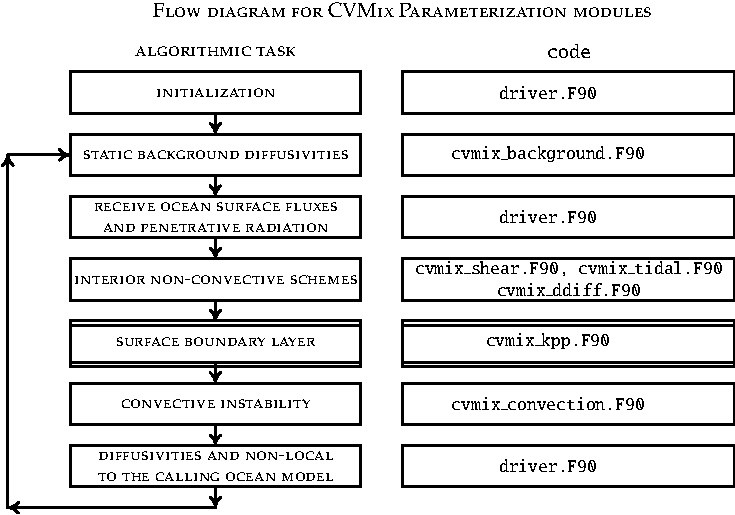
\includegraphics[angle=0,width=15cm]{./mfpic_figs/cvmix_flow_diagram.pdf}
\caption[Flow diagram for CVMix schemes]{\sf This flow diagram depicts
  the general algorithmic steps required to utilize the CVMix
  parameterization modules.  The initialization step occurs in the
  ocean model (e.g., MPAS-ocean, MOM, or POP) calling the CVMix
  modules.  This initialization serves to set up arrays and derived
  type structures, all as a function of the input that it receives
  from the calling ocean model code.  The next step during
  initialization is to call the module {\tt cvmix\_background.F90} to
  fill chosen static background diffusivities.  Upon entering the time
  dependent portion of the ocean model integration, the driver
  receives surface fluxes and penetrative radiative fluxes.  Calls are
  made to chosen interior non-convective mixing schemes, such as shear
  mixing, tide mixing, and double diffusion.  Thereafter, the surface
  boundary layer scheme is called, with KPP the scheme targetted for
  Phase I of CVMix.  If implementing the KPP scheme according to
  \cite{LargeKPP}, then the boundary layer calculation {\it must} come
  after the interior non-convective portion, and before the convective
  portion (see discussion in Section
  \ref{section:vert_mix_schemes_ordering_cvmix}).  If instead using
  the simpler approach detailed in Section
  \ref{subsection:kpp-shape-function}, then KPP can be called in any
  order within the calling tree.  After the boundary layer, then
  convective mixing is called, with regions of gravitationally
  unstable water given a large diffusivity.  Notably, if KPP is used
  for the surface boundary layer, parameterized convective mixing is
  generally performed only beneath the KPP boundary layer.  The final
  step returns the diffusivity $K_{\lambda}$, viscosity, and non-local
  transport $K^{\mbox{\tiny non-local}}_{\lambda} \; \gamma_{\lambda}$
  (equation (\ref{eq:non-local-transport-intro})), arrays to the
  calling ocean model code.  A new time step starts by reinitializing
  the diffusivities to their static background values.}
\label{fig:vertical_mix_flow_cvmix}
\end{center}
\rule{\textwidth}{0.005in}
\end{figure}
%%%%%%%%%%%%%%%%%%%%%%%%%%%%%%%%%%%%%%%%%%%%%%%%%%%%%%%%%%%%%%%%%%%%%%%%




\chapter{\scshape Elements of CVMix parameterizations}
\label{chapter:cvmix_elements}

\minitoc
\vspace{.5cm}

\begin{mdframed}[backgroundcolor=lightgray!50]
We present in this chapter certain elements required for computing
CVMix parameterizations.  Details specific to particular schemes are
provided in later chapters.
\end{mdframed}




\section{Discrete vertical grid}
\label{section:vertical-grid-numerics}

As part of the numerical discretizations used by CVMix modules, we
have need to describe how discrete fields are placed on a vertical
grid, and how finite difference operations are performed.  A vertical
column generally has time dependent positions of the discrete fields,
distances between the positions, and thicknesses of the cells over
which the discrete fields are defined.  Generality is necessary for
models where grid cell thicknesses are functions of time, and CVMix
allows for such freedom.

Figure \ref{fig:cvmix_discrete_vertical} provides a schematic of the
conventions for a tracer column used by CVMix modules. The conventions
are motivated by those used in MOM and POP, yet some details may
differ slightly.  A summary of the choices made in developing this
figure are as follows.
\begin{itemize}

\item {\sc vertical coordinate and depth}: The vertical coordinate $z$ increases
  upward and extends from the ocean bottom at $z=-H(x,y)$ to the sea
  surface at $z = \eta(x,y,t)$
\begin{equation}
   -H(x,y) \le z \le \eta(x,y,t).
\end{equation}
Conversely, the {\it depth} 
\begin{equation}
   d = -z + \eta 
\label{eq:depth-defined}
\end{equation} 
increases from a value of $d=0$ at $z=\eta$ to $d = H+\eta$ at $z=-H$
\begin{equation}
  0 \le   d \le H+\eta. 
\end{equation}
So in summary, depth increases when moving down into the ocean
starting from the free surface, and $z$ increases moving up from a
resting ocean at $z=0$.

\item {\sc height coordinate}: The height vertical coordinate is
  defined as minus the depth
\begin{equation}
   {\cal  H}  = -d = z - \eta 
\label{eq:height-defined}
\end{equation} 
and so represents the height above the sea surface.  In the ocean, the
height is negative (liquid ocean sits beneath the sea surface), and
sits within the range of values
\begin{equation}
  -(H+\eta) \le  {\cal  H}  \le 0.
\end{equation}
For the CVMix implementation of the KPP scheme detailed in Chapter
\ref{chapter:cvmix_kpp}, the code assumes the vertical coordinate
provided by the calling routine is the height, so that the CVMix code
does not need to be given the sea level field.
  
\item {\sc tracer cell arrays}: Tracer cell arrays are labelled with
  the discrete index {\tt kt}, and have dimensions {\tt nlevs}.  The
  index {\tt kt} increases downward starting from {\tt kt} =1 for the
  top model grid cell.  The number of wet points, {\tt nlevs}, is a
  function of the column.  Examples of tracer cell arrays include
  temperature, salinity, pressure, density, thermal expansion
  coefficient, and haline contraction coefficient.

\item {\sc w-cell or interface arrays}: W-cell or interface arrays are
  labelled with the discrete index {\tt kw}, and have dimensions {\tt
    nlevs+1}.  The index {\tt kw} increases downward starting from
  {\tt kw} =1 at the top ocean interface.  The notation ``w-cell''
  originates from the continuity equation, in which the vertical
  velocity component, $w$, transfers mass or tracer across the
  vertical interfaces of tracer cells.  Examples of w-cell or
  interface arrays are diffusivity, viscosity, vertical tracer
  derivatives, buoyancy frequency, and Richardson number.  For most
  w-cell arrays, both the top interface at {\tt kw=1} and bottom
  interface at {\tt kw=nlevs+1} have zero values.

  One argument for using {\tt nlevs+1} interfaces is that we avoid
  ambiguity of where the data resides. Interface arrays of size {\tt
    nlevs} could start at either the top or bottom of the first grid
  cell and, even if well documented, the ambiguity will increase the
  potential for code errors.  It does not matter so much whether
  interface arrays are dimensioned {\tt 0:nlevs} or {\tt 1:nlevs+1};
  there is only one way the data could be laid out relative to the
  tracer arrays which have dimensions {\tt 1:nlevs}. Yet the reason to
  prefer {\tt 1:nlevs+1} is that this dimensioning simplifies
  declarations and argument passing, given the standard assumptions
  made by Fortran in laying out memory for arrays.

 
\item {\sc tracer cell thickness}: The rectangular boxes in Figure
  \ref{fig:cvmix_discrete_vertical} represent tracer cells whose
  thickness is measured by the array element {\tt dzt(kt)} with units
  of meter. This array has dimensions {\tt dzt(nlevs)}.  These
  thicknesses are generally time dependent.  The array {\tt dzt} is an
  input to CVMix, passed from the ocean model each time step.

\item {\sc w-cell thickness or tracer point separation}: The array
  {\tt dzw} has dimensions {\tt dzw(nlevs+1)}.  The array element {\tt
    dzw(kw=1)} measures distance (in meters) from the top of the top
  tracer cell to the tracer point {\tt T(kt=1)}, and array element
  {\tt dzw(kw=nlevs+1)} measures the distance from the bottom tracer
  point {\tt T(kt=nlevs)} to the bottom of the bottom tracer cell.
  Intermediate elements of {\tt dzw} measure the distance between
  tracer points, or equivalently the thickness of a w-cell.  These
  distances are generally time dependent.  The array {\tt dzw} is an
  input to CVMix, passed from the ocean model each time step.

\item {\sc distance from ocean surface to tracer cell point}: The
  distance (in meters) from the tracer cell point to the ocean surface
  is given by the array element {\tt zt(kt)}.  This array has
  dimensions {\tt zt(nlevs)}.  If needed, the array {\tt zt} is
  constructed inside CVMix code based on the values of {\tt dzt} and
  {\tt dzw}. 

\item {\sc distance from ocean surface to interface}: The distance
  from the tracer cell interface, or the w-point, to the ocean surface
  is given by the array element {\tt zw(kw)}.  This array has
  dimensions {\tt zw(nlevs+1)}.  If needed, the array {\tt zw} is
  constructed inside CVMix code based on the values of {\tt dzt} and
  {\tt dzw}.

\end{itemize}



%%%%%%%%%%%%%%%%%%%% %%%%%%%%%%%%%%%%%%%%%%%%%
\begin{figure}[h!t]
\rule{\textwidth}{0.005in}
\begin{center}
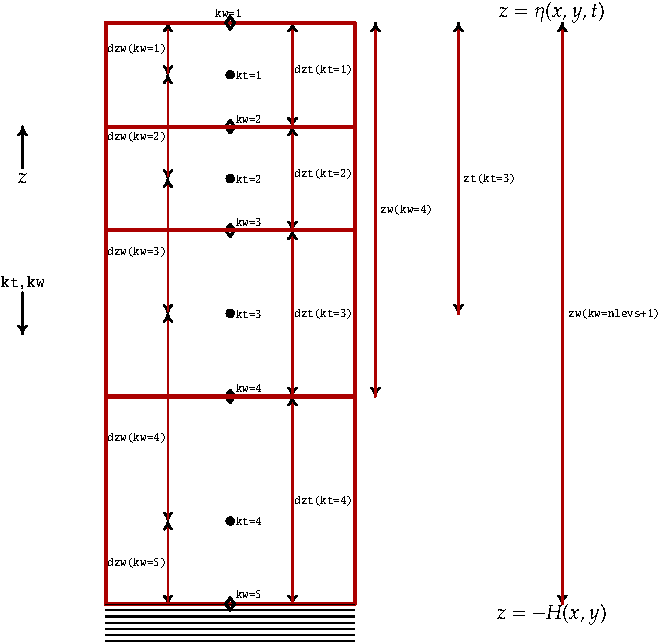
\includegraphics[angle=0,width=10cm]{./mfpic_figs/cvmix_discrete_vertical.pdf}
\caption[Discrete vertical column for CVMix modules]{\sf Schematic of
  a discrete vertical column used in CVMix modules, with the surface
  at $z=\eta(x,y,t)$ and bottom at $z=-H(x,y)$.  The vertical
  coordinate $z$ increases upward, whereas the discrete vertical
  indices {\tt kt} and {\tt kw} increase downward.  CVMix code assumes
  distances and thicknesses are in units of meters. The rectangular
  boxes represent tracer cells in the ocean model.  The array element
  {\tt dzt(kt)} measures the thickness of a tracer cell. This array
  has dimensions {\tt dzt(nlevs)}, where {\tt nlevs} is the number of
  wet cells in a particular column.  For this particular example, {\tt
    nlevs} = 4.  The array {\tt dzw} has dimensions {\tt
    dzw(nlevs+1)}.  The array element {\tt dzw(kw=1)} measures the
  distance from the top of the top tracer cell to the tracer point
  {\tt T(kt=1)}, and array element {\tt zw(kw=nlevs+1)} measures the
  distance from the bottom tracer point {\tt T(kt=nlevs)} to the bottom
  of the bottom tracer cell.  Intermediate elements of {\tt dzw}
  measure the distance between tracer points, or equivalently the
  thickness of w-cells.  The distance from the ocean surface to a
  tracer point is measured by the array element {\tt zt(kt)}, and the
  distance to the interface is measured by {\tt zw(kw)}.  The total
  thickness of a column is {\tt zw(nlevs+1)}, and it is generally time
  dependent, as are all of the grid distances {\tt dzt} and {\tt dzw}.
  Arrays that are defined at the interface, such as buoyancy
  frequency, Richardson number, diffusivity, viscosity, have vertical
  indices {\tt kw}.  Arrays defined at the tracer cell point, such as
  temperature, salinity, and density, have vertical indices {\tt kt}.}
\label{fig:cvmix_discrete_vertical}
\end{center}
\rule{\textwidth}{0.005in}
\end{figure}
%%%%%%%%%%%%%%%%%%%%%%%%%%%%%%%%%%%%%%%%%%%%%%%%%%%%%%%%%%%%%%%%%%%%%%%%


\section{Gravitational stability}
\label{section:buoyancy-frequency-elements}

Buoyancy stratification plays a key role in physical ocean proceses.
We have need to quantify stratification for use in CVMix
parameterizations, along with the associated gravitational stability
of a water column.  For this purpose, we introduce the notion of an
adiabatic and isohaline parcel displacement, from which we develop an
algorithm for computing the buoyancy frequency used to measure
vertical stratification.  The notions detailed here should be
respected by the calling ocean model in order for the CVMix modules to
produce physically relevant results.
\begin{mdframed}[backgroundcolor=lightgray!50]
\begin{quote}
  {\sf The squared buoyancy frequency, $N^2$, is an input to CVMix
    modules.}
\end{quote}
\end{mdframed}


\subsection{Density change under infinitesimal displacements}

Consider a displacement $\mathrm{d}{\bf x}$ of a fluid parcel.  To
leading order, the {\it in situ} density at the new point is related
to the reference density by
\begin{equation}
 \rho({\bf x} + \mathrm{d} \, {\bf x})= \rho({\bf x}) + \mathrm{d}\rho({\bf x}).
\end{equation}
Using the leading order term in a Taylor series expansion, the density
increment can be approximated by
\begin{subequations}
\begin{align}
\mathrm{d}\rho &=  \rho({\bf x} + \mathrm{d} \, {\bf x}) - \rho({\bf x})
 \\
 &\approx \mathrm{d}{\bf x} \cdot \nabla \rho
 \\
 &= \rho \, \mathrm{d}{\bf x} \cdot \rho^{-1} \, \nabla \rho
\\
&= 
\rho \, \mathrm{d}{\bf x} \cdot 
 \left( -\alpha \, \nabla \Theta + \beta \, \nabla  S  + \frac{\nabla p}{\rho \, c_{\mbox{\tiny sound}}^{2}  } \right),
\end{align}
\label{eq:full-density-increment-displacement}
\end{subequations}
where all terms on the right hand side are evaluated at the reference
point ${\bf x}$.  To reach this expression, we introduced the thermal
expansion coefficient
\begin{equation}
 \alpha = -\frac{1}{\rho}\left( \frac{\partial \rho}{\partial \Theta} \right),
\label{eq:alpha-elements}
\end{equation}
the haline contraction coefficient 
\begin{equation}
 \beta = \frac{1}{\rho}\left( \frac{\partial \rho}{\partial S} \right),
\label{eq:beta-elements}
\end{equation}
and the squared sound speed
\begin{equation}
 c^{2}_{\mbox{\tiny sound}} = \left( \frac{\partial p}{\partial \rho}\right).
\label{eq:sound-speed-elements}
\end{equation}
The ambient density at the new point, $\rho({\bf x} + \mathrm{d} {\bf
  x})$, thus differs from density at the reference point, $\rho({\bf
  x})$, by an amount $\mathrm{d}\rho({\bf x})$ according to
\begin{equation}
 \rho({\bf x} + \mathrm{d} \, {\bf x}) - \rho({\bf x}) = 
 \rho({\bf x}) \, \mathrm{d}{\bf x} \cdot 
 \left( -\alpha \, \nabla \Theta + \beta \, \nabla  S  + \frac{ \nabla p }{\rho \, c_{\mbox{\tiny sound}}^{2}  }\right).
\end{equation}


\subsection{Neutral directions}
\label{subsection:neutral-directions}

Parcel displacements associated with mixing will change the parcel's
temperature, salinity, and concentration of other material
tracers. Rather than considering such mixing processes, we here wish
to know if through buoyancy forces alone, a particular parcel
displacement is favored, resisted, or neutral.  For this purpose, we
introduce the notion of a displacment restricted to adiabatic and
isohaline conditions (i.e., no heat or salt exchanged during the
parcel displacement).  Such displacements occur in the absence of
mechanical energy needed for mixing.  Our goal is thus to determine
{\it neutral} directions, whereby non-dissipative motion occurs in the
absence of buoyancy forces.

The density change associated with an adiabatic and isohaline
displacement is determined just by pressure changes arising from the
displacement, so that
\begin{equation}
\rho({\bf x} + \mathrm{d} {\bf x})_{\mbox{\tiny  adiabatic/isohaline}} - \rho({\bf x})  =
  \rho \, \mathrm{d}{\bf x} \cdot  \left( \frac{ \nabla p }{\rho \, c_{\mbox{\tiny sound}}^{2}  } \right).
\label{eq:infinitesimal-rho-adiabatic}
\end{equation}
This density change occurs merely through the pressure dependence of
{\it in situ} density.  Operationally, to compute $\rho({\bf x} +
\mathrm{d} {\bf x})_{\mbox{\tiny adiabatic/isohaline}}$, we may choose
to evaluate the right hand side of equation
(\ref{eq:infinitesimal-rho-adiabatic}), or we may evaluate the
equation of state at the temperature and salinity of the reference
point, ${\bf x}$, but with pressure at the displaced point, ${\bf x} +
\mathrm{d} {\bf x}$
\begin{equation}
  \rho({\bf x} + \mathrm{d} {\bf x})_{\mbox{\tiny adiabatic/isohaline}} 
 = \rho[ \Theta({\bf x}), S({\bf x}), p({\bf x}  + \mathrm{d} {\bf x})]. 
\end{equation}
The difference in density between a parcel undergoing an adiabatic and
isohaline displacement, $\rho({\bf x} + \mathrm{d} {\bf x})_{\mbox{\tiny
    adiabatic/isohaline}}$, and the density of the ambient environment,
$\rho({\bf x} + \mathrm{d} {\bf x})$, is thus given by
\begin{subequations}
\begin{align}
\rho({\bf x} + \mathrm{d} {\bf x})  - \rho({\bf x} + \mathrm{d} {\bf x})_{\mbox{\tiny  adiabatic/isohaline}} 
&=
\rho[ \Theta({\bf x} + \mathrm{d} {\bf x}), S({\bf x} + \mathrm{d} {\bf x}), p({\bf x} + \mathrm{d} {\bf x})]
-
\rho[ \Theta({\bf x} ), S({\bf x}), p({\bf x} + \mathrm{d} {\bf x})]
\\
&=
  \rho \, \mathrm{d}{\bf x} \cdot 
  \left( -\alpha \, \nabla \Theta + \beta \, \nabla  S \right),
\end{align}
\label{eq:neutral-directions-motivated}
\end{subequations}
where the final equality ignores higher order terms in the Taylor
series.  If a parcel makes an adiabatic and isohaline excursion and
finds itself in a region where the ambient density is unchanged, then
there are no buoyancy forces to resist that displacement.  Directions
defined by such displacements are termed {\it neutral directions}
\citep{McDougall1987a}.  By definition, neutral directions are
orthogonal to the local dia-neutral unit vector
\begin{equation}
 \hat{\gamma} = \left( \frac{-\alpha \, \nabla \Theta + \beta \, \nabla S}
                          {|-\alpha \, \nabla \Theta + \beta \, \nabla S|}
 \right),
\end{equation}
 so that 
\begin{equation}
\rho({\bf x} + \mathrm{d} {\bf x})  - \rho({\bf x} + \mathrm{d} {\bf x})_{\mbox{\tiny  adiabatic/isohaline}} 
 = 
 \left( \rho \, \mathrm{d}{\bf x} \cdot \hat{\gamma} \right) \, 
 |-\alpha \, \nabla \Theta + \beta \, \nabla  S |. 
\end{equation}


\subsection{Squared buoyancy frequency}
\label{subsection:buoyancy-frequency-and-stability}

When measuring the gravitational stability of a fluid column, we are
concerned with vertical displacements and the resistence from buoyancy
stratification to such displacements.  To anticipate the needs of the
discrete calculation, we assume knowledge of the density, tracer
concentration, and pressure at depths $z$ and $z+\mathrm{d}z$ (see
Figure \ref{fig:cvmix_stability}).


\subsubsection{Stability to upward displacements from a deeper reference point}

Consider first an upward displacement starting from the reference
depth $z$ and going to $z+\mathrm{d}z$.  Following the notation of
Figure \ref{fig:cvmix_stability}, we have
\begin{equation}
\rho(z+\mathrm{d} z)  - \rho(z+\mathrm{d} z)_{\mbox{\tiny adiabatic/isohaline}}  
= 
 \rho[ \Theta(z + \mathrm{d} z), S(z + \mathrm{d} z), p(z + \mathrm{d} z)]
-
\rho[ \Theta(z), S(z), p(z + \mathrm{d}z)].
\end{equation}
As for the case of a general displacement considered in Section
\ref{subsection:neutral-directions}, we perform a Taylor series
expansion about the reference depth at $z$ to render the leading order
identity
\begin{equation}
\begin{split}
\rho(z+\mathrm{d} z)  - \rho(z+\mathrm{d} z)_{\mbox{\tiny adiabatic/isohaline}}  
&\approx 
  \rho(z) \, \mathrm{d}z \, \left[ 
   -\alpha(z) \, \left( \frac{\partial \Theta}{\partial z} \right )
 + \beta(z) \, \left( \frac{\partial S}{\partial z} \right) \right]
 \\
&= 
 -\left( \frac{\rho \, \mathrm{d}z}{g} \right) \, N^{2}.
\end{split}
\label{eq:infinitesimal-delta-rho-elements-upwards}
\end{equation}
The final equality in equation
(\ref{eq:infinitesimal-delta-rho-elements-upwards}) introduced the
squared buoyancy frequency
 \begin{equation}
 N^{2}_{\mbox{\scriptsize linear}} = g \, \left( \alpha \, \frac{\partial \Theta}{\partial z} 
                         - \beta  \, \frac{\partial S}{\partial z} \right),
\label{eq:buoyancy-frequency-elements}
\end{equation}
where the vertical derivatives and expansion coefficients are
evaluated at the deep reference point $z$.  Calculating gravitational
stability according to the linear approximate expresson
(\ref{eq:buoyancy-frequency-elements}) is accurate so long as all
higher order terms in the Taylor series approximation can be
neglected.  It is for this reason we denote this a linear
approximation to the buoyancy frequency.  The higher order terms are
potentially important in regions where the equation of state becomes
quite nonlinear, such as the high latitudes of the Southern Ocean.  So
we do not generally recommend the linear approximation for global
modeling.  Instead, we recommend use of the full squared buoyancy
frequency
\begin{equation}
\begin{split}
 N^{2}_{\mbox{\scriptsize full}}(z \rightarrow z+\mathrm{d}z) &\equiv 
 -\left( \frac{g}{\mathrm{d}z} \right) 
   \left( \frac{\rho(z+\mathrm{d} z)  - \rho(z+\mathrm{d} z)_{\mbox{\tiny adiabatic/isohaline}} } {\rho(z) } \right)
\end{split}
\label{eq:infinitesimal-delta-rho-elements-upwards-B}
\end{equation}

Again, the calculation
(\ref{eq:infinitesimal-delta-rho-elements-upwards-B}) will determine
gravitational stability of an upward parcel displacement from depth
$z$ to $z+\mathrm{d}z$.  To further expose the physics of this
calculation, consider two vertical stratifications.
\begin{itemize}
\item {\sc gravitationally stable stratification:
    $N^{2}_{\mbox{\scriptsize full}}(z \rightarrow z+\mathrm{d}z) >
    0$}: In this case, a vertically upward displacement occurring
  without heat or salt exchange will produce a parcel density that is
  more than the ambient density: $\rho(z+\mathrm{d} z) -
  \rho(z+\mathrm{d} z)_{\mbox{\tiny adiabatic/isohaline}} <0$. This
  particular adiabatic and isohaline displacement is resisted by
  buoyancy forces.  A displaced parcel will exhibit oscillatory motion
  with squared frequency $N^{2}_{\mbox{\scriptsize full}}(z
  \rightarrow z+\mathrm{d}z)$ (see Section 2.9.1 of
  \cite{Vallis2006}).  The vertical density profile is thus
  gravitationally stable.

\item {\sc gravitationally unstable stratification:
    $N^{2}_{\mbox{\scriptsize full}}(z \rightarrow z+\mathrm{d}z) <
    0$}: Now the upward adiabatic and isohaline displacement leads to
  a lesser density than the ambient environment: $\rho(z+\mathrm{d} z)
  - \rho(z+\mathrm{d} z)_{\mbox{\tiny adiabatic/isohaline}} >0$.  This
  particular adiabatic and isohaline displacement is encouraged by
  buoyancy forces to rise even further. The vertical density profile
  is thus gravitationally unstable.

\end{itemize}

\begin{figure}
\rule{\textwidth}{0.005in}
\begin{center}
\resizebox{5cm}{!}{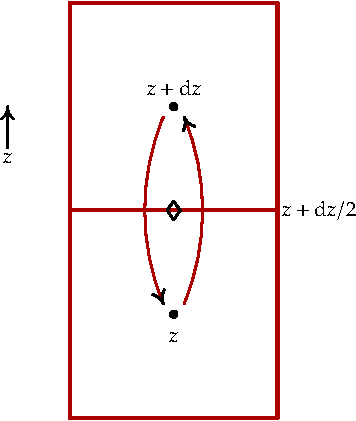
\includegraphics{./mfpic_figs/cvmix_stability.pdf}}
\caption[Parcel displacements for gravitational stability calculation]
{Illustration of how parcels are displaced when checking for the
  gravitational stability. As for the discrete column shown in Figure
  \ref{fig:cvmix_discrete_vertical}, we assume knowledge of the tracer
  and pressure values at the tracer points $z$ and
  $z+\mathrm{d}z$. Two displacements are considered: one vertically up
  and one vertically down.  The notation corresponds on the discrete
  grid of Figure \ref{fig:cvmix_discrete_vertical}, where
  $z+\mathrm{d}z$ in the present figure corresponds to an interface
  depth {\tt zw(kw)}; the deeper point at $z$ corresponds to the
  tracer point {\tt zt(kt+1)}; and the shallower point $z+\mathrm{d}z$
  corresponds to the tracer point {\tt zt(kt)}.}
\label{fig:cvmix_stability}
\end{center}
\rule{\textwidth}{0.005in}
\end{figure}


\subsubsection{Stability to downward displacements from a shallower reference point}

We now determine the gravitational stability of fluid to displacements
from a shallow reference point $z^{*} = z + \mathrm{d}z$ downward to
$z$, which requires the calculation
\begin{equation}
\begin{split}
\rho(z)  - \rho(z)_{\mbox{\tiny adiabatic/isohaline}}  
&= 
 \rho[ \Theta(z), S(z), p(z)]
-
\rho[ \Theta(z+\mathrm{d}z), S(z+\mathrm{d}z), p(z)]
\\
 &=
 \rho[ \Theta(z^{*}-\mathrm{d}z), S(z^{*}-\mathrm{d}z), p(z)]
-
\rho[ \Theta(z^{*}), S(z^{*}), p(z)]
\\
&\approx 
 -\rho \, \mathrm{d}z \, \left[ 
   -\alpha \, \left( \frac{\partial \Theta}{\partial z} \right )
  + \beta \, \left( \frac{\partial S}{\partial z} \right) \right]
 \\
&=
\left( \frac{\rho \, \mathrm{d}z}{g} \right) \, N^{2},
\end{split}
\label{eq:infinitesimal-delta-rho-elements-downward}
\end{equation}
where terms in the final two equalities are evaluated at the shallow
reference point $z^{*} = z + \mathrm{d}z$.  Following equation
(\ref{eq:infinitesimal-delta-rho-elements-upwards-B}), we introduce the
full squared buoyancy frequency
\begin{equation}
\begin{split}
 N^{2}_{\mbox{\scriptsize full}}(z +\mathrm{d}z \rightarrow z) &\equiv 
 \left( \frac{g}{\mathrm{d}z} \right) 
 \left( \frac{\rho(z)  - \rho(z)_{\mbox{\tiny adiabatic/isohaline}} } {\rho(z+\mathrm{d}z) } \right).
\end{split}
\label{eq:infinitesimal-delta-rho-elements-downwards}
\end{equation}



\subsubsection{Combined displacements to approximate gravitational stability at
  interface depth}

Let us summarize the two previous results.  Again, we have two tracer
points at depths $z$ and $z+\mathrm{d}z$.  Gravitational stability can
be probed in two separate ways. First we consider the deeper depth $z$
as a reference point and displace parcels vertically upward to
$z+\mathrm{d}z$.  This calculation leads to the squared buoyancy
frequency at the reference point $z$
\begin{equation}
\begin{split}
 N^{2}_{\mbox{\scriptsize full}}(z \rightarrow z + \mathrm{d}z)
 &=
 -\left( \frac{g}{\mathrm{d}z} \right)
  \left(  \frac{\rho(z+\mathrm{d} z)  - \rho(z+\mathrm{d} z)_{\mbox{\tiny adiabatic/isohaline}} }{\rho(z) } \right)
\\
&=
 -\left( \frac{g}{\mathrm{d}z } \right)  \left( 
 \frac{\rho[ \Theta(z + \mathrm{d} z), S(z + \mathrm{d} z), p(z + \mathrm{d} z)]
-
\rho[ \Theta(z), S(z), p(z + \mathrm{d}z)] }{\rho(z)}
\right).
\end{split}
\label{eq:infinitesimal-delta-rho-elements-upwards-summary}
\end{equation}
We next the shallower depth $z+\mathrm{d}z$ as a reference point and
displace parcels vertically downward to $z$.  This calculation leads
to the squared buoyancy frequency at the reference point
$z+\mathrm{d}z$
\begin{equation}
\begin{split}
 N^{2}_{\mbox{\scriptsize full}}(z + \mathrm{d}z \rightarrow z)
 &=
 \left( \frac{g}{\mathrm{d}z} \right)
 \left(  \frac{ \rho(z)  - \rho(z)_{\mbox{\tiny adiabatic/isohaline}}  }{\rho(z+\mathrm{d}z)  } \right)  
 \\
 &=
 \left( \frac{g}{\mathrm{d}z } \right) 
 \left( \frac{ \rho[ \Theta(z), S(z), p(z)]- \rho[ \Theta(z+\mathrm{d}z), S(z+\mathrm{d}z), p(z)]
  }{\rho(z+\mathrm{d}z)}  
\right).
\end{split}
\label{eq:infinitesimal-delta-rho-elements-downward-summary}
\end{equation}
We now use these two results to render an approximation to the squared
buoyancy frequency at the interface point $z + \mathrm{d}z/2$, which
is where the discrete calculation requires the stability to be
estimated (Section \ref{subsubsection:numerics-buoyancy-frequency}).
For this purpose, we take the average to yield an expression in terms
of density differences \small
\begin{equation}
\begin{split}
&N^{2}_{\mbox{\scriptsize full}}(z+\mathrm{d}z/2) 
 \equiv 
 \frac{N^{2}_{\mbox{\scriptsize full}}(z \rightarrow z + \mathrm{d}z) + N^{2}_{\mbox{\scriptsize full}}(z + \mathrm{d}z \rightarrow z)}{2}
\\
&= -\frac{g}{2 \, \mathrm{d}z} 
  \left( 
 \frac{
    \rho[ \Theta(z + \mathrm{d} z), S(z + \mathrm{d} z), p(z + \mathrm{d} z)]
  -\rho[ \Theta(z), S(z), p(z + \mathrm{d}z)]
  }{\rho(z) }
 \; - \; 
 \frac{ \rho[ \Theta(z), S(z), p(z)]-
 \rho[ \Theta(z+\mathrm{d}z), S(z+\mathrm{d}z), p(z)]
  }{\rho(z+\mathrm{d}z) }
 \right).
\end{split}
\label{eq:n2-in-terms-of-density-differences}
\end{equation}
\normalsize As a sanity check, note that if the density is independent
of pressure, and we replace densities in the denominator with the
constant reference density $\rho_{o}$ as commonly done for the
Boussinesq approximation (see Section 2 of \cite{Roquet_etal2014}), we
have the familiar simplified result
\begin{equation}
N^{2}(z+\mathrm{d}z/2) = -\frac{g}{\mathrm{d}z} 
  \left( 
 \frac{ \rho[ \Theta(z + \mathrm{d} z), S(z + \mathrm{d} z)]  -\rho[ \Theta(z), S(z)]  }{\rho_{o}}
 \right)    \qquad   \mbox{density independent of pressure}.
\end{equation}


\subsubsection{Linear approximation: not recommended in general}

Instead of computing the full buoyancy frequency in terms of density
differences, one may choose to make a linearization of the expansion
following equation (\ref{eq:buoyancy-frequency-elements}), in which we
write
\begin{equation}
\begin{split}
N^{2}_{\mbox{\scriptsize linear}} (z+\mathrm{d}z/2) 
&\equiv \frac{N^{2}_{\mbox{\scriptsize linear}} (z) + N^{2}_{\mbox{\scriptsize linear}} (z+\mathrm{d}z)}{2}
\\
&= 
 g \, \left( \overline{\alpha}^{z}  \, \frac{\partial \Theta}{\partial z} 
               -\overline{\beta}^{z} \,  \frac{\partial S}{\partial z} \right),
\end{split}
\label{eq:n2-in-terms-of-tracers}
\end{equation} 
where we introduced the vertical averaging operator to bring the
expansion coefficients from the tracer point to the interface
\begin{equation}
  \overline{\alpha}(z+\mathrm{d}z/2) = \frac{\alpha(z) + \alpha(z+\mathrm{d}z)}{2}.
\end{equation}
The vertical tracer derivatives are naturally placed on the vertical
cell interface.  Contrary to the density difference approach of
equation (\ref{eq:n2-in-terms-of-density-differences}), the expression
(\ref{eq:n2-in-terms-of-tracers}) requires no non-standard
calculations of the equation of state.  What it does require is
calculation of the thermal expansion coefficients, with that
calculation also used for neutral physics.  So the expression
(\ref{eq:n2-in-terms-of-tracers}) may be somewhat more computationally
efficient.  Nonetheless, when used as a measure of gravitational
stability, the expression
(\ref{eq:n2-in-terms-of-density-differences}) makes less assumptions
about our ability to truncate the Taylor series at the leading order.
This truncation may become problematic particularly in high latitudes
where the equation of state can become quite nonlinear.  Hence, we
generally do not recommend use of the linear expression
(\ref{eq:n2-in-terms-of-tracers}) for the calculation of water column
stability.


\subsubsection{Discrete calculation of the squared buoyancy frequency}
\label{subsubsection:numerics-buoyancy-frequency}

CVMix modules do {\it not} compute the buoyancy frequency.  Rather,
the calling model does and then passes $N^{2}$ to CVMix. Nonetheless,
CVMix modules must assume a placement for the buoyancy frequency, with
the following choice made:
\begin{mdframed}[backgroundcolor=lightgray!50]
\begin{quote}
  {\sf CVMix modules assume the squared buoyancy frequency, $N^{2}$,
      lives at the vertical interface of tracer cells, following the
      convention given by Figure \ref{fig:cvmix_discrete_vertical}.}
\end{quote}
\end{mdframed}
We now write the buoyancy frequency expression
(\ref{eq:n2-in-terms-of-density-differences}) in terms of discrete
indices for ready incorporation into a numerical model, in which we have 
\scriptsize
\begin{mdframed}[backgroundcolor=lightgray!50]
\begin{equation}
N^{2}({\tt kw}) = 
 -\left( \frac{g}{2 \,  {\tt dzw(kw)} } \right) 
  \left( 
 \frac{
    \rho[ \Theta( {\tt kt}), S( {\tt kt}), p( {\tt kt})]
  -\rho[ \Theta( {\tt kt+1} ), S({\tt kt +1} ), p( {\tt kt} )]
  }{\rho({\tt kt+1} ) }
 \; -  \; 
 \frac{ \rho[ \Theta({\tt kt+1}), S({\tt kt+1}), p({\tt kt+1})]-
 \rho[ \Theta({\tt kt} ), S( {\tt kt}), p({\tt kt+1})]
  }{\rho( {\tt kt}) }
 \right).
\label{eq:n2-in-terms-of-density-differences-discrete}
\end{equation}
\end{mdframed}
\normalsize Note that by referring to Figures
\ref{fig:cvmix_discrete_vertical} and \ref{fig:cvmix_stability}, we
see that the discrete label {\tt kt} corresponds to the shallower
point $z+\mathrm{d}z$, whereas {\tt kt+1} corresponds to the deeper
point $z$.  This correspondence is made when converting equation
(\ref{eq:n2-in-terms-of-density-differences}) to
equation (\ref{eq:n2-in-terms-of-density-differences-discrete}).


\section{Gradient Richardson number}
\label{section:gradient-richardson-number-elements}

The gradient Richardson number measures the ratio of the stabilizing
effects from buoyancy stratification to the destabilizing effects from
vertical shear
\begin{equation}
  \mbox{Ri}= \frac{N^{2} }{ |\partial_{z} \, {\bf u}|^{2} }.
\label{eq:flux-Richardson-elements}
\end{equation}
In this equation, $N^{2}$ is the squared buoyancy frequency, whose
discrete calculation was detailed in Section
\ref{subsubsection:numerics-buoyancy-frequency}.  The denominator
contains the squared vertical shear of the horizontal velocity,
$|\partial_{z} \, {\bf u}|^{2}$.  When the Richardson number is small,
say below 1/4 as in \cite{miles1961}, the flow tends toward a
turbulent state via production of Kelvin-Helmholz
instabilities.\footnote{The critical Richardson number, below which
  instabilities are enabled, may need to be artificially set larger
  than the canonical 1/4 when considering discrete approximations to
  the velocity shear.  The reason is that we are unable to precisely
  compute the vertical shear on a finite grid.  See Section 4b of
  \cite{Jacksonetal2008} for discussion.}  Consequently, many vertical
mixing schemes make use of the Richardson number, such as the shear
mixing schemes presented in Chapter \ref{chapter:cvmix_shear}.
Additionally, the KPP boundary layer scheme (Chapter
\ref{chapter:cvmix_kpp}) makes use of a bulk Richardson number used to
define properties of the surface planetary boundary layer (Section
\ref{subsection:kpp-obl-thickness}).

As for the squared buoyancy frequency $N^{2}$, the CVMix modules do
{\it not} compute a Richardson number, since details of this
calculation depend on choices regarding the grid layout in the ocean
model.  Rather, the Richardson number is an input to CVMix modules.
CVMix modules assume a placement for the Richardson number, with the
following choice made:
\begin{mdframed}[backgroundcolor=lightgray!50]
\begin{quote}
  {\sf The gradient Richardson number, $\mbox{Ri}$, is an input to
    CVMix modules.  CVMix modules assume the gradient Richardson
    number lives at the vertical interface of tracer cells, following
    the convention given by Figure
    \ref{fig:cvmix_discrete_vertical}.}
\end{quote}
\end{mdframed}

Staggering of tracer and velocity fields on a discrete grid leads to
ambiguity for how to compute a discrete Richardson number.  The issue
is the squared buoyancy frequency in the numerator naturally lives at
the vertical interface between tracer grids (Section
\ref{subsubsection:numerics-buoyancy-frequency}), whereas the
horizontal positioning for the denominator depends on the chosen
horizontal staggering of velocity.  We detail here some possible
methods for the B-grid and C-grid.  Unstructured grids used by
MPAS-ocean require further considerations.  Each grid involves
averaging operations specific to the grid in order to compute the
shear.  There are even further methods available if we choose a
different discrete placement of $N^{2}$ beyond that discussed in
Section \ref{subsubsection:numerics-buoyancy-frequency}.


\subsection{Considerations for the B-grid}
\label{subsection:b-grid-richardson-number}

Figure \ref{fig:b-grid} illustrates the horizontal arrangement of
prognostic model fields used with the B-grid. The B-grid places both
horizontal prognostic velocity components at the same point, the
corner of the tracer cell.  This placement is natural when computing
the Coriolis Force.  However, it is unnatural for computation of
advective tracer transport or the horizontal pressure gradient force
acting on velocity.  The need to perform an averaging operation when
computing the horizontal pressure gradient leads to the computational
mode associated with gravity waves on the B-grid (\cite{Mesinger1973},
\cite{KillworthFreesurf1991}, \cite{MOM3manual},
\cite{GriffiesPacSchmidtBalaji2001}, and Section 12.9 of
\cite{SMGbook}).

\begin{figure}
\rule{\textwidth}{0.005in}
\begin{center}
\resizebox{7cm}{!}{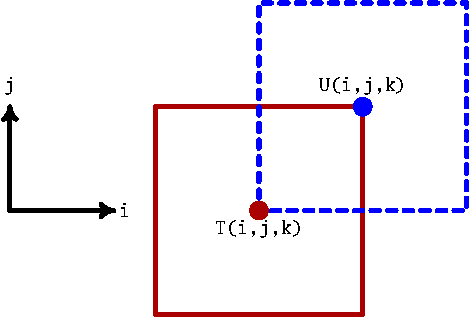
\includegraphics{./mfpic_figs/B_grid.pdf}}
\caption[Placement of fields onto the B-grid] {Illustration of how
  fields are placed on the horizontal B-grid using a {\it northeast
    convention}.  Velocity points {\tt U(i,j,k)} are placed to the
  northeast of tracer points {\tt T(i,j,k)}.  Both horizontal velocity
  components $u_{i,j,k}$ and $v_{i,j,k}$ are placed at the velocity
  point {\tt U(i,j,k)}.  Both the tracer point and velocity point have
  a corresponding grid cell region, denoted by the solid and dashed
  squares.}
\label{fig:b-grid}
\end{center}
\rule{\textwidth}{0.005in}
\end{figure}

We present here some methods for computing the squared vertical shear
of the horizontal velocity on the B-grid, and thus methods for
computing the Richardson number.
\begin{itemize}

\item {\sc T-grid average of U-grid velocity}: The first approach
  computes a horizontal average of the velocity field to place it onto
  the T-grid, and then computes the vertical derivative and its
  square.  The 4-point horizontal average to compute a T-grid velocity
  is written
\begin{equation}
  {\bf u}^{\mbox{\tiny T}}  = \overline{\bf u}^{x,y}.
\end{equation}
Note that this, and all, four point averages do {\it not} include land
points. We next compute the squared vertical shear with the T-grid
horizontal velocity for use in the Richardson number calculation
\begin{equation}
    \mbox{Ri}^{(\mbox{\tiny Ba})} = \frac{N^{2}} { \left| \frac{\partial {\bf u}^{\mbox{\tiny T}}}{\partial z} \right|^{2} }.
\end{equation}

\item {\sc T-grid average of U-grid shear}: A slight modification of
  the $\mbox{Ri}^{(\mbox{\tiny Ba})}$ calculation takes the T-grid
  horizontal average of the U-grid shear
\begin{equation}
  \left( \frac{\partial {\bf u}}{\partial z} \right)^{\mbox{\tiny T}}
  = \overline{ \left( \frac{\partial {\bf u}}{\partial z} \right)}^{x,y},
\end{equation}
and then computes the square so that
\begin{equation}
    \mbox{Ri}^{(\mbox{\tiny Bb})} = \frac{N^{2}} { \left|  \left( \frac{\partial {\bf u}}{\partial z} \right)^{\mbox{\tiny T}} \right|^{2} }.
\end{equation}
With uniform vertical grid spacing, the two Richardson number
calculations are the same
\begin{equation}
 \mbox{Ri}^{(\mbox{\tiny Ba})} = \mbox{Ri}^{(\mbox{\tiny Bb})}  \qquad \mbox{uniform vertical grid spacing.}
\end{equation}

\item {\sc T-grid average of squared U-grid shear}: The third method
  computes the squared shear on the original U-grid, and then averages
  the squared shears onto the T-grid
\begin{equation}
  \left( \left| \frac{\partial {\bf u}}{\partial z} \right|^{2} \right)^{\mbox{\tiny T}}
  = \overline{  \left( \left| \frac{\partial u}{\partial z}  \right|^{2}  
     +  \left| \frac{\partial v}{\partial z}  \right|^{2}  \right)  }^{x,y},
\end{equation}
so that 
\begin{equation}
    \mbox{Ri}^{(\mbox{\tiny Bc})} = \frac{N^{2}} { \left( \left| \frac{\partial {\bf u}}{\partial z} \right|^{2} \right)^{\mbox{\tiny T}}}.
\end{equation}

\end{itemize}



\subsection{Considerations for the C-grid}
\label{subsection:c-grid-richardson-number}

Figure \ref{fig:c-grid} illustrates the horizontal arrangement of
prognostic model fields used with the C-grid. The C-grid places the
zonal velocity component on the zonal tracer cell face, and meridional
velocity component on the meridional tracer cell face.  This placement
is suited for computation of advective tracer transport.  It is also
suited for computing the stress tensor and the horizontal pressure
gradient force acting on velocity components.  However, it is not
natural for computation of the Coriolis Force.  The need to perform an
averaging operation to compute the Coriolis Force leads to the
presence of a computational null mode associated with geostrophically
balanced flow \citep{Adcroftetal1999}.

\begin{figure}
\rule{\textwidth}{0.005in}
\begin{center}
\resizebox{7cm}{!}{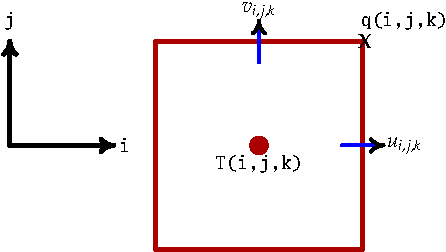
\includegraphics{./mfpic_figs/C_grid.pdf}}
\caption[Placement of fields onto the C-grid] {Illustration of how
  fields are placed on the horizontal C-grid.  We illustrate here the
  convention that the zonal velocity component $u_{i,j,k}$ sits at the
  east face of the tracer cell {\tt T(i,j)}, and the meridional
  velocity component $v_{i,j,k}$ sits at the north face of the tracer
  cell {\tt T(i,j,k)}.  This convention follows the {\it northeast}
  convention also used for the B-grid.}
\label{fig:c-grid}
\end{center}
\rule{\textwidth}{0.005in}
\end{figure}


We present here some methods for computing the squared vertical shear
of the horizontal velocity on the C-grid, and thus methods for
computing the Richardson number. 
\begin{itemize}

\item {\sc T-grid average of u,v-grid velocity components}: The first
  approach considered computes a horizontal average of the $u,v$
  velocity components to place both onto the T-grid, and then computes
  the vertical derivative and its square.  The horizontal averaging
  requires a two-point average so that 
\begin{equation}
  (u^{\mbox{\tiny T}}, v^{\mbox{\tiny T}}) = (\overline{u}^{x}, \overline{v}^{y}).
\end{equation}
As for the B-grid averaging considered in Section
\ref{subsection:b-grid-richardson-number}, all averages considered
here do {\it not} include land points. The squared vertical shear with
the T-grid horizontal velocity is then used for the Richardson number
calculation
\begin{align}
 \left| \frac{\partial {\bf u}^{\mbox{\tiny T}}}{\partial z} \right|^{2}
 &= \left( \frac{\partial \overline{u}^{x}}{\partial z} \right)^{2} 
     +
     \left( \frac{\partial \overline{v}^{y}}{\partial z} \right)^{2} 
\\
    \mbox{Ri}^{(\mbox{\tiny Ca})} &= \frac{N^{2}} { \left| \frac{\partial {\bf u}^{\mbox{\tiny T}}}{\partial z} \right|^{2} }.
\end{align}


\item {\sc T-grid average of u,v-grid shear}: A slight modification of
  the $\mbox{Ri}^{(\mbox{\tiny Ca})}$ calculation takes the T-grid
  horizontal average of the u,v-grid shear
\begin{equation}
  \left( \frac{\partial {\bf u}}{\partial z} \right)^{\mbox{\tiny T}}
  = 
  \left[  \overline{ \left( \frac{\partial u}{\partial z} \right)}^{x}, \overline{ \left( \frac{\partial v}{\partial z} \right)}^{y}
   \right],
\end{equation}
and then computes the square so that
\begin{equation}
    \mbox{Ri}^{(\mbox{\tiny Cb})} = \frac{N^{2}} { \left|  \left( \frac{\partial {\bf u}}{\partial z} \right)^{\mbox{\tiny T}} \right|^{2} }.
\end{equation}
With uniform vertical grid spacing, the two Richardson number
calculations are the same
\begin{equation}
 \mbox{Ri}^{(\mbox{\tiny Ca})} = \mbox{Ri}^{(\mbox{\tiny Cb})}  \qquad \mbox{uniform vertical grid spacing.}
\end{equation}

\item {\sc T-grid average of squared u,v-grid shear}: The third method
  computes the squared shear on the original u,v-grid, and then averages
  the squared shears onto the T-grid
\begin{equation}
  \left( \left| \frac{\partial {\bf u}}{\partial z} \right|^{2} \right)^{\mbox{\tiny T}}
  = \overline{  \left| \frac{\partial u}{\partial z} \right|^{2}   }^{x}
    +
   \; \; \overline{ \left| \frac{\partial v}{\partial z} \right|^{2}  }^{y}
\end{equation}
so that 
\begin{equation}
    \mbox{Ri}^{(\mbox{\tiny Bc})} = \frac{N^{2}} { \left( \left| \frac{\partial {\bf u}}{\partial z} \right|^{2} \right)^{\mbox{\tiny T}}}.
\end{equation}


\end{itemize}


\chapter{\scshape Sample chapter for CVMix documentation}
\label{chapter:cvmix_MODULE}

\minitoc
\vspace{.5cm}

\begin{mdframed}[backgroundcolor=lightgray!50]
  This chapter provides a sample for what is useful to include in the
  CVMix documentation of a physical parameterization scheme.  Clear
  and complete CVMix documentation is critical for the intelligent use
  of any scheme, so the author should focus on creating documentation
  that is useful and pedagogical.  The following CVMix Fortran module
  is directly connected to the material in this chapter:
\begin{align*} 
 &{\tt cvmix\_MODULE.F90}
\end{align*}
\end{mdframed}

Here are some suggestions for writing this document.
\begin{itemize}

\item Aim for a level of concise pedagogy, so that the reader will
  readily understand the scheme, but without going into too many
  details that are available in published literature.  Some of the
  other CVMix chapters are good examples of this philosophy (e.g.,
  tide mixing chapter \ref{chapter:cvmix_tidal}), though others are
  not (e.g., KPP chapter \ref{chapter:cvmix_kpp}).

\item This chapter should describe any test cases available from the
  scheme, including sample figures.  Test cases allow the new user to
  verify a particular implementation, and to provide a sample of how
  the physical parameterizion works.

\item Add new bibliography entries to the .bib file in the directory
  {\tt cvmix\_manual/references}.

\item Figures associated with this document should ideally be named
  {\tt new\_scheme\_figure\_number.pdf} or the like, thus making it
  simpler to associate a figure with a chapter.

\end{itemize}



\section{Introduction to the mixing scheme}
\label{section:intro_new_scheme}

This section provides a broad overview of the scheme, focusing on the
scientific background and the processes available from the CVMix
module.  


\section{Theory}
\label{section:theory_new_scheme}

This section develops the basic theory for the scheme, summarizing
elements of the published literature in a manner that provides an
intellectual foundation for the CVMix scheme.  The reader should
understand what the scheme aims to do from a physics perspective.  

\section{Numerical implementation in CVMix}
\label{section:numerics_new_scheme}

This section develops the numerical implementation choices made for
the CVMix implementation.  Please include here a full description of
options for using the scheme, as well as a list of parameters and
their physical dimensions.  Recommended usage and test cases can be
presented here as well.  


\section{Further sections}

The above template is clearly insufficient for some purposes.  Feel
free to modify as you see appropriate.  


 
\chapter{\scshape Static background schemes}
\label{chapter:cvmix_background}


\minitoc
\vspace{.5cm}

\begin{mdframed}[backgroundcolor=lightgray!50]
This chapter presents options in CVMix code for prescribing static
(time independent) background diffusivities and viscosities.  The
following CVMix Fortran module is directly connected to the material
in this chapter:
\begin{align*} 
 &{\tt cvmix\_background.F90}
\end{align*}
\end{mdframed}

\section{Options for static background mixing coefficients}
\label{section:background-diffusivities}

\cite{Jochum2009} describes the large sensitivities found in climate
model simulations to the choice of background vertical diffusivities.
There are various options in CVMix code for specifying a static
background diffusivity and viscosity.  These mixing coefficients are
generally a function of space but remain the same value throughout the
simulation, and so are independent of the flow state.  These static
values are primarily determined for tracer diffusivity, with a Prandtl
number (ratio of diffusivity to viscosity) used to determine the
background viscosity.  A common choice for Prandtl number is 10,
although for some background diffusivities there is no corresponding
background viscosity (i.e., zero Prandtl number).


\section{The profile from Bryan-Lewis (1979)} 
\label{section:bryan-lewis}

A classic choice for background diffusivity is that proposed by
\cite{BryanLewis1979}, which has an arctangent form with smaller
values in the upper ocean and larger values beneath a pivot depth,
originally set to 1500~m
\begin{equation}
 \kappa_{\mbox{\tiny Bryan-Lewis}} = {\tt vdc1}
   + {\tt vdc2}  \;  \arctan\left[ ( |z| - {\tt dpth}) \,   {\tt linv}  \, \right].
\label{eq:bryan-lewis-function-pop}
\end{equation}
This is the form appearing in POP, where the parameters are defined as
follows.
\begin{itemize}

\item {\tt vdc1} is the diffusivity (squared length per time) at $|z|
  = {\tt dpth}$,

\item {\tt vdc2} = amplitude of variation for the diffusivity
  (squared length per time)

\item {\tt linv} is an inverse length scale 

\item {\tt dpth} is the vertical depth where the diffusivity equals
  {\tt vdc1}.

\end{itemize}
All lengths and diffusivities should be in MKS units.  In many
implementations, such as for GFDL-CM2.1, there is no corresponding
Bryan-Lewis viscosity, so the corresponding Bryan-Lewis Prandtl number
is zero.  But more generally, the viscosity is computed according to a
chosen Prandtl number.

In MOM5 and earlier versions of MOM, the form
(\ref{eq:bryan-lewis-function-pop}) is written in the somewhat more
cumbersome manner for historical reasons
\begin{equation}
 \kappa_{\mbox{\tiny Bryan-Lewis}} = {\tt convert} \left( 
       \,{\tt afkph}
   +  ({\tt dfkph}/\pi)  \; \arctan\left[ {\tt sfkph} (100 \,  |z| - {\tt zfkph} ) \right]
    \right),
\label{eq:bryan-lewis-function-mom}
\end{equation}
where {\tt afkph}, {\tt dfkph}, {\tt sfkph}, and {\tt zfkph} are
tunable constants, and ${\tt convert} = 1 \, \times
10^{-4}~\mbox{m}^{2}\mbox{s}^{-1}$ converts from the original CGS to
MKS.  The mapping between the MOM and POP forms
(\ref{eq:bryan-lewis-function-pop}) is given by the following
\begin{align}
{\tt vdc1} &= \kappa_{o} \, {\tt afkph}
\\
 {\tt vdc2} &= \kappa_{o} \, {\tt dfkph}/\pi
\\
 {\tt linv}     &= 100 \, {\tt sfkph}
\\
 {\tt dpth} &= 100 \, {\tt zfkph}.
\end{align}
We provide this mapping since Figure \ref{fig:bryan_lewis-profiles}
was constructed using the original MOM-based form.  Shown are two
examples of vertical diffusivity profiles used in the GFDL-CM2.1
simulations \citep[see][for discussion]{OMDT2005a}, with the values
given by 
\begin{align}
{\tt afkph} &=0.75
 \\
{\tt dfkph} &=0.95
\\
{\tt sfkph} &=4.5 \, \times 10^{-5}
\\
{\tt zfkph} &=2500
\label{fig:bryan_lewis-profiles-polar}
\end{align}
and for the equatorial region they are 
\begin{align}
{\tt afkph} &=0.65
\\
 {\tt dfkph} &=1.15
\\
 {\tt sfkph} &= 4.5 \, \times 10^{-5}
\\
 {\tt zfkph} &=2500.
\label{fig:bryan_lewis-profiles-tropics}
\end{align}



%%%%%%%%%%%%%%%%%%%% %%%%%%%%%%%%%%%%%%%%%%%%%
\begin{figure}[h!t]
\rule{\textwidth}{0.005in}
\begin{center}
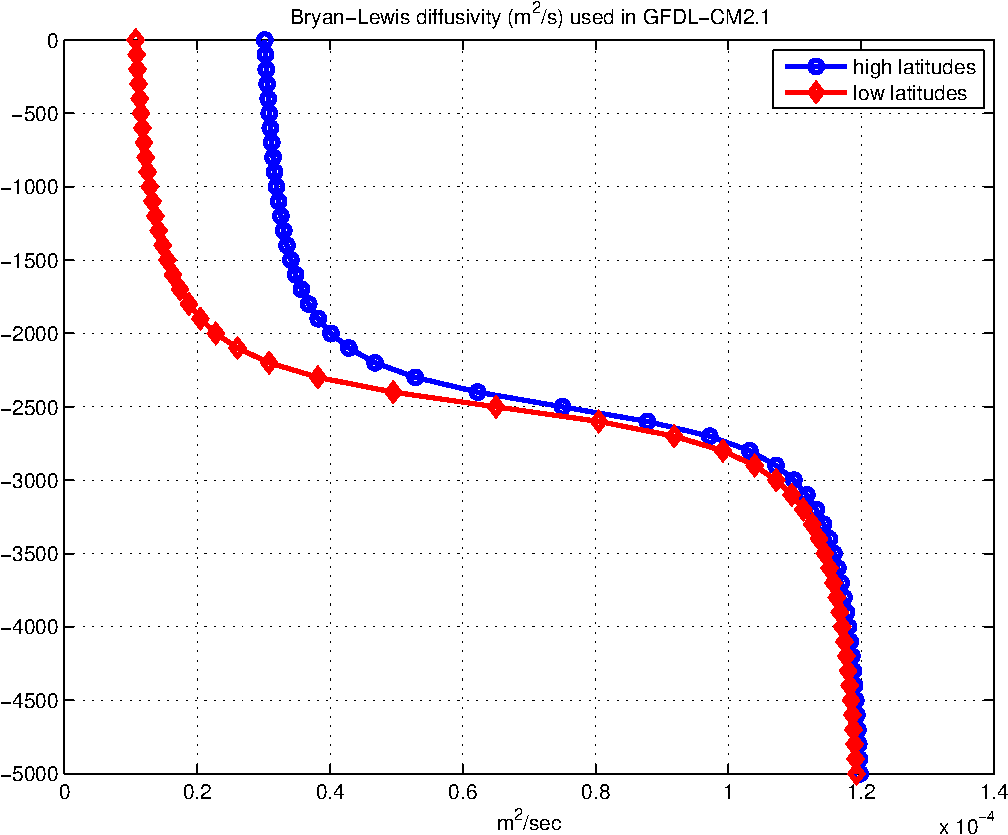
\includegraphics[angle=0,width=8cm]{./figs/bryan_lewis_cm2p1.pdf}
\caption[Bryan-Lewis background diffusivities]{\sf Sample vertical
  profiles for background diffusivities (in units of
  $\mbox{m}^{2}~\mbox{s}^{-1}$) given by the \cite{BryanLewis1979}
  functional form, as used by the OM3 ocean component of the
  GFDL-CM2.1 climate model \citep{OMDT2005a}.  The surface values in
  the tropics are $0.1 \times 10^{-4} \, \mbox{m}^2 \, \mbox{s}^{-1}$,
  whereas they are increased in the high latitudes to $0.3 \times
  10^{-4} \, \mbox{m}^2 \, \mbox{s}^{-1}$.
The Bryan-Lewis coefficients from equation
(\ref{eq:bryan-lewis-function-mom}) for the high latitudes are given
by 
${\tt afkph} =0.75$,
${\tt dfkph} =0.95$,
${\tt sfkph} =4.5 \, \times 10^{-5}$,
${\tt zfkph} =2500$,
and for the equatorial region they are 
${\tt afkph} =0.65$,
${\tt dfkph} =1.15$,
${\tt sfkph} = 4.5 \, \times 10^{-5}$,
${\tt zfkph} =2500$. }
\label{fig:bryan_lewis-profiles}
\end{center}
\rule{\textwidth}{0.005in}
\end{figure}
%%%%%%%%%%%%%%%%%%%%%%%%%%%%%%%%%%%%%%%%%%%%%%%%%%%%%%%%%%%%%%%%%%%%%%%%

The original implementation from \cite{BryanLewis1979} chose the
background as a function only of depth.  However, the CM2.1
implementation shown in Figure \ref{fig:bryan_lewis-lat-depth}
provides an exponential transition from the lower latitude form to the
higher latitude form, with the transition latitude taken as
$35^{\circ}$.  In this way, the background diffusivity is a function
of both latitude and depth.  The resulting diffusivity is shown in
Figure \ref{fig:bryan_lewis-lat-depth}.

%%%%%%%%%%%%%%%%%%%% %%%%%%%%%%%%%%%%%%%%%%%%%
\begin{figure}[h!t]
\rule{\textwidth}{0.005in}
\begin{center}
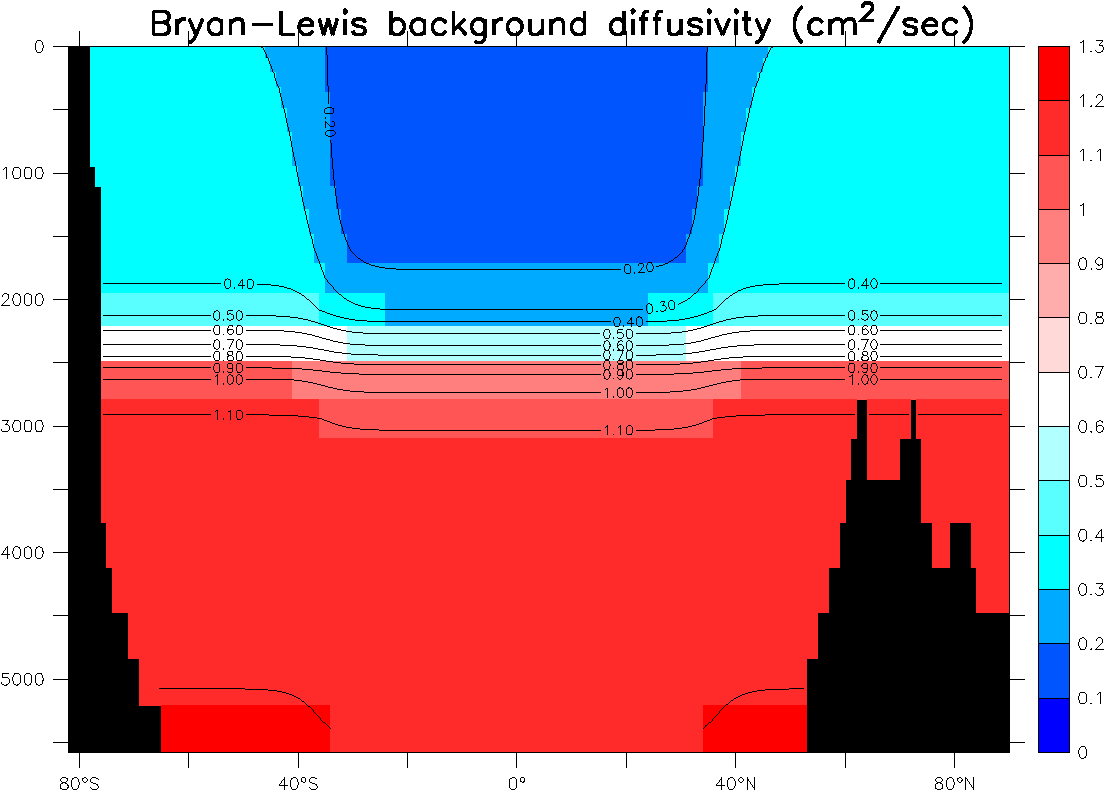
\includegraphics[angle=0,width=8cm]{./figs/bl_diffusivity.pdf}
\caption[Latitude-depth Bryan-Lewis diffusivity]{Shown here is the
  latitude dependent Bryan-Lewis diffusivity
  ($\mbox{cm}^{2}~\mbox{s}^{-1}$) based on values used in GFDL-CM2.1
  configuration discussed in \cite{OMDT2005a}.  The diffusivity is
  composed of the two profiles shown in Figure
  \ref{fig:bryan_lewis-profiles}, with an exponential transition at
  $35^{\circ}$ from the lower values in the tropics to the larger
  values in the high latitudes.}
\label{fig:bryan_lewis-lat-depth}
\end{center}
\rule{\textwidth}{0.005in}
\end{figure}
%%%%%%%%%%%%%%%%%%%%%%%%%%%%%%%%%%%%%%%%%%%%%%%%%%%%%%%%%%%%%%%%%%%%%%%%


\section{The profile from Henyey et al. (1986)} 
\label{section:henyey-diffusivity}

To be completed.  
\chapter{\scshape Parameterized shear induced mixing}
\label{chapter:cvmix_shear}

\minitoc
\vspace{.5cm}

\begin{mdframed}[backgroundcolor=lightgray!50]
  In this chapter we detail the CVMix version of those
  parameterizations arising from shear induced mixing in stratified
  flows.  The following CVMix Fortran module is directly connected to
  the material in this chapter:
\begin{align*} 
 &{\tt cvmix\_shear.F90}
\end{align*}
\end{mdframed}

\section{Mixing from shear instability}
\label{section:shear-instability-mixing}

Shear induced mixing occurs when vertical shears in the horizontal
velocity overcome the stabilizing effects from vertical buoyancy
stratification.  Shear instability is governed by the local or
gradient Richardson number discussed in Section
\ref{section:gradient-richardson-number-elements}
\begin{equation}
 \mbox{Ri} = \frac{N^{2}}{|\partial_{z} \, {\bf u}|^{2} }.
\label{eq:richardson-number}
\end{equation}
In this expression, $N^{2}$ is the squared buoyancy frequency (Section
\ref{section:buoyancy-frequency-elements}), with a linear
approximation given by
\begin{equation}
 N^{2}_{\mbox{\scriptsize linear}} 
 = g \, \left( \alpha \, \frac{\partial \Theta}{\partial z} 
                         - \beta  \, \frac{\partial S}{\partial z} \right).
\label{eq:buoyancy-frequency-shear}
\end{equation}
We assume throughout that the water is stably stratified, so that
$N^{2} > 0$.  With $N^{2} < 0$, one should set the diffusivity and
viscosity to a large value to parameterize mixing associated with the
gravitational instability.

The denominator in the Richardson number in equation
(\ref{eq:richardson-number}) is the squared vertical shear of the
horizontal velocity vector resolved by the model grid
\begin{equation}
 |\partial_{z} \, {\bf u}|^{2}  =
  \left( \frac{\partial u}{\partial z} \right)^{2} 
 +
 \left( \frac{\partial V}{\partial z} \right)^{2}. 
\end{equation}
When the Richardson number is below a critical value, $\mbox{Ri} <
\mbox{Ri}_{c}$, shear instabilities can grow to initiate turbulence,
which in turn leads to enhanced mixing.

The canonical value of the critical gradient Richardson number is
\begin{equation}
 \mbox{Ri}_{c} =1/4   \qquad \mbox{analytical value from shear layer instability.} 
\end{equation}
This value corresponds to the critical value for initiation of a
Kelvin-Helmholz instability in a shear layer \citep{miles1961}.
However, as reviewed in Section 4b of \cite{Jacksonetal2008}, there
are many reasons that 1/4 is not always the optimal value to use in
numerical simulations.  Thus, most schemes choose noticeably larger
values, which allows for shear-induced mixing to be intiated in less
unstable regions of the model's resolved flow.




\section{Pacanowski and Philander mixing}
\label{section:shear-instability-parameterized-ppvmix}

An early form for parameterized shear mixing is that proposed by
\cite{PPvmix}, where their application focused on equatorial dynamics.
They used a different viscosity, $\nu_{\mbox{\tiny pp shear}}$, and
diffusivity, $\kappa_{\mbox{\tiny pp shear}}$.  For gravitationally
stable profiles (i.e., $N^{2} > 0$), they chose
\begin{align}
 \nu_{\mbox{\tiny pp shear}}&= \frac{\nu_{0}}{(1 + a  \, \mbox{Ri})^{n}} 
\\
 \kappa_{\mbox{\tiny pp shear}}&= \frac{\nu_{0}}{(1 + a  \, \mbox{Ri})^{n+1}}, 
\end{align}
where $\nu_{0}$, $a$ and $n$ are adjustable parameters.  Common
settings used in POP are $a=5$ and $n=2$.  Note that the Prandtl
number is not constant using this prescription
\begin{subequations}
\begin{align}
  \mbox{Pr}_{\mbox{\scriptsize pp}} &= \frac{\nu_{\mbox{\tiny pp shear}}}{\kappa_{\mbox{\tiny pp  shear}}} 
 \\
 &= 1 + a  \, \mbox{Ri}.
\end{align}
\end{subequations}


\section{Richardson number mixing from \cite{LargeKPP}}
\label{section:shear-instability-parameterized-kpp}

For regions beneath the KPP boundary layer (see Figure
\ref{fig:boundary-layer-schematic-kpp}), \cite{LargeKPP} and
\cite{Large_Gent1999} parameterized shear induced mixing using the
following diffusivities
\begin{equation}
  \kappa_{\mbox{\tiny kpp shear}}= \left\{
\begin{array}{llll}
&\kappa_{0}  &\mbox{Ri} < 0  &\mbox{gravitational instability regime} 
 \\
   &\kappa_{0} \left[1- \left(\frac{\mbox{Ri}}{\mbox{Ri}_0}\right)^2 \right]^3
   &0 < \mbox{Ri}  <  \mbox{Ri}_0   &\mbox{shear instability regime}
\\
 &0 &\mbox{Ri} \ge \mbox{Ri}_{0} &\mbox{stable regime.} 
\end{array}
 \right.
\label{eq:kappa-shear-kpp}
\end{equation}
The form in the shear instability regime falls most rapidly near
$\mbox{Ri} = 0.4 \, \mbox{Ri}_{0}$, which aims to parameterize the
onset of shear instability. In this neighborhood, rapid changes in
$\mbox{Ri}$ can cause gravitational instabilities to develop in the
vertical, but these are largely controlled by vertically smoothing
$\mbox{Ri}$ profiles with a $1-2-1$ smoother.  Unlike \cite{PPvmix},
\cite{LargeKPP} chose a unit Prandtl number for shear induced mixing;
i.e., the shear induced viscosity is the same as the shear induced
diffusivity
\begin{subequations}
\begin{align}
  \mbox{Pr}_{\mbox{\scriptsize kpp}} &= \frac{\nu_{\mbox{\tiny kpp shear}}}{\kappa_{\mbox{\tiny kpp  shear}}} 
 \\
 &= 1.
\end{align}
\end{subequations}


\chapter{\scshape Energetically based mixing schemes from tidal dissipation}
\label{chapter:cvmix_tidal}


\minitoc
\vspace{.5cm}

\begin{mdframed}[backgroundcolor=lightgray!50]
  This chapter summarizes the CVMix implementation of the
  parameterized vertical mixing associated with mechanical energy
  dissipation from tidal motions in both the ocean interior and near
  the bottom.  The following CVMix Fortran module is directly
  connected to the material in this chapter:
\begin{align*} 
 &{\tt cvmix\_tidal.F90}
\end{align*}
\end{mdframed}

\section{Introduction to tidal induced mixing}
\label{section:vert_tidal_intro}

Mixing arises when mechanical energy dissipates at the small scales in
the presence of a nonzero gradient of tracer and/or momentum.  There
are two sources of mechanical energy dissipation considered in this
chapter.
\begin{itemize}

\item {\sc Internal waves in ocean interior}: Breaking internal
  gravity waves arise when barotropic tidal flow is scattered into
  internal tidal energy. This process occurs when astronomical tides
  interact with rough bottom topography.

\item {\sc Tidal waves interacting with continental shelves}:
  Frictional bottom drag is enhanced as tides encounter continental
  shelves (whose depths are generally 500~m or less).  There is an
  associated mixing of water masses due to this dissipation.

\end{itemize}
To resolve both of these dissipation processes explicitly in a
numerical model requires grid resolution no coarser than meters in the
vertical (throughout the water column), and 1-10 kilometers in the
horizontal.  This very fine resolution is not generally accessible to
global climate models, so it is necessary to consider a
parameterization.

CVMix has implementations for the following tide mixing
parameterizations.
\begin{itemize}
 
\item {\sc baroclinic or internal wave mixing}: \cite{Simmonsetal2004}
  presented the first implementation in an ocean climate model of an
  internal tide mixing parameterization.  \cite{Jayne2009} followed
  with an updated implementation.  A more recent study by
  \cite{Melet_etal_2013} implemented the ideas from \cite{Polzin2009}
  to remove the arbitrariness of the vertical deposition function used
  by \cite{Simmonsetal2004} and \cite{Jayne2009}.  Any of these
  schemes aim to provide a physically based replacement for the static
  vertical diffusivity of \cite{BryanLewis1979} (Chapter
  \ref{chapter:cvmix_background}).

\end{itemize}
Although CVMix provides an optional Prandtl number, it is general
practice to assume a unit Prandtl number for each of the tide
parameterization schemes.\footnote{The Prandlt number is the ratio of
  viscosity to diffusivity.}



\section{Energetic elements of tide mixing parameterizations}
\label{section:vert_tidal_formulation}

We now consider elements of how energetic based tide mixing
parameterizations are formulated.


\subsection{Bottom drag}
\label{subsection:bottom-drag-barotropic-tides}

Frictional bottom drag is typically parameterized as
\begin{equation}
  {\bf D}_{\mbox{\tiny bottom drag}} = C_{D} \, {\bf u} \, | {\bf u}|
  \qquad \mbox{(units of $\mbox{m}^{2}~\mbox{s}^{-2}$),}
\end{equation}
where $C_{D}$ is a dimensionless drag coefficient with a value on the
order of
\begin{equation}
C_{D} \approx  2 \times 10^{-3}. 
\end{equation}
Energy dissipation associated with this bottom drag is given by
\begin{equation}
 E_{\mbox{\tiny bottom drag}} =
  \rho_{o} \, {\bf u} \cdot {\bf D}_{\mbox{\tiny bottom drag}} 
 = \rho_{o} \, |{\bf u}|^{3}
\qquad \mbox{(units of $\mbox{W} \; \mbox{m}^{-2}$),}
\label{eq:energy-dissipation-bottom-drag-general}
\end{equation}
where $\rho_{o}$ is a reference ocean density.  

A component to the energy dissipation
(\ref{eq:energy-dissipation-bottom-drag-general}) is associated with
barotropic tides as they encounter the ocean bottom, particularly
continental shelves and other shallow ocean regions.  In an ocean
model that does not represent the astronomical tides, we may choose to
enhance the model's bottom velocity through a root-mean-square tidal
speed,$U_{\mbox{\tiny tide}}$, so that the bottom drag takes the form
\begin{equation}
  {\bf D}_{\mbox{\tiny bottom drag}} = 
  C_{D} \, {\bf u} \, \left( {\bf u}^{2} + U_{\mbox{\tiny tide}}^{2} \right)^{1/2},
\end{equation}
where now the velocity ${\bf u}$ refers to the model's resolved bottom
velocity field.  The modified energy dissipation from bottom drag
thus takes the form
\begin{equation}
 E_{\mbox{\tiny bottom drag}} =  \rho_{o} \, C_{D} \,  {\bf u}^{2} \, \left( {\bf u}^{2} + U_{\mbox{\tiny tide}}^{2} \right)^{1/2}.
\label{eq:energy-dissipation-bottom-drag-with-tides}
\end{equation}
The tidal speed $U_{\mbox{\tiny tide}}$ may be a prescribed global
constant, as in the OCCAM simulations from \cite{Webbetal1998}.  It
may instead be a map determined by an offline tide model, as in
\cite{Jayne_etal2001}.  Or, it may be computed online by periodically
running a tide model during the update of the primitive equation ocean
model.


\subsection{Wave drag from breaking internal gravity waves}

A drag associated with breaking internal gravity waves was written by
\cite{Jayne_etal2001} as
\begin{equation}
  {\bf D}_{\mbox{\tiny wave drag}} = (1/2) \, N_{\mbox{\tiny bott}}\,  
  \kappa_{\mbox{\tiny topo}} \, h_{\mbox{\tiny topo}}^{2} \, {\bf u}
\qquad \mbox{(units of $\mbox{m}^{2} \; \mbox{s}^{-2}$),}
\end{equation}
where $N_{\mbox{\tiny bott}}$ is the buoyancy frequency at the ocean
bottom, and $(\kappa_{\mbox{\tiny topo}},h_{\mbox{\tiny topo}})$ are
wavenumber (dimensions of inverse length) and amplitude (dimensions of
length) scales for the topography.  The product $\kappa_{\mbox{\tiny
    topo}} \, h_{\mbox{\tiny topo}}^{2}$ has dimensions of length and
defines a {\em roughness length}
\begin{equation}
  L_{\mbox{\tiny rough}} = \kappa_{\mbox{\tiny topo}} \, h_{\mbox{\tiny topo}}^{2}  
\label{eq:roughness-length}
\end{equation}
to be specified according to statistics of the observed ocean bottom
topography.  The internal wave drag can thus be written as
\begin{equation}
  {\bf D}_{\mbox{\tiny wave drag}} = (1/2) \, N_{\mbox{\tiny bott}}  \,  L_{\mbox{\tiny rough}} \, {\bf u}
\qquad \mbox{(units of $\mbox{m}^{2} \; \mbox{s}^{-2}$).}
\end{equation}

The energy dissipation associated with breaking internal gravity waves
is given by
\begin{equation}
\begin{split}
 E_{\mbox{\tiny wave drag}} &=
  \rho_{o} \, \langle {\bf u} \cdot {\bf D}_{\mbox{\tiny wave drag}} \rangle 
 \\
 &=
   (\rho_{o}/2) \, N_{\mbox{\tiny bott}}  \,  L_{\mbox{\tiny rough}}
   \,  \langle {\bf u}^{2} \rangle  
 \qquad \mbox{(units of $\mbox{W} \; \mbox{m}^{-2}$).}
\end{split}
\label{eq:wave-energy-flux}
\end{equation}
In the \cite{Jayne_etal2001} paper, they emphasize that
$\kappa_{\mbox{\tiny topo}}$, which sets the roughness length through
$L_{\mbox{\tiny rough}} = \kappa_{\mbox{\tiny topo}} \, h_{\mbox{\tiny
    topo}}^{2}$, is used as a tuning parameter, with the tide model
tuned to give sea level values agreeing with observations.  Then, the
energy dissipation can be diagnosed from the tide model.

As with the bottom drag (Section
\ref{subsection:bottom-drag-barotropic-tides}), the wave energy
dissipation arises from energy removed from the barotropic tides, yet
here it is transferred into baroclinic tides.  Some of the energy
transferred into the baroclinic tides dissipates locally due to local
wave breaking, and this dissipation then leads to enhanced local
mixing.  The remaining baroclinic energy propogates away; i.e., it is
non-local.  The ratio of local to non-local energy is not well known,
and is the focus of research.


\subsection{Relating dissipation to mixing via \cite{Osborn1980}}

Mixing occurs when mechanical energy is dissipated in the presence of
stratification.  The relation between energy dissipation and mixing is
not known from first principles, so we consider dimensional arguments
to establish a useful form.  Since we are concerned with vertical
mixing, we assume that diffusivity is inversely proportional to the
vertical stratification, with stratification strength measured by the
buoyancy frequency, $N^{2}$ (see Section
\ref{subsection:buoyancy-frequency-and-stability}).  Mechanical energy
per mass has units of $\mbox{m}^{2}~\mbox{s}^{-2} =
\mbox{J}~\mbox{kg}^{-1}$, and the dissipation of this energy, written
as $\epsilon$, has units of $\mbox{m}^{2}~\mbox{s}^{-3} =
\mbox{W}~\mbox{kg}^{-1}$
\begin{equation}
\epsilon = \mbox{mechanical energy dissipation in units of
 $\mbox{m}^{2}~\mbox{s}^{-3} = \mbox{W}~\mbox{kg}^{-1}$.}
\label{eq:energy-dissipation-epsilon}
\end{equation}
Together, the energy dissipation and buoyancy frequency define a
diffusivity given through the relation \citep{Osborn1980}
\begin{equation}
  \kappa_{\mbox{\tiny dissipate}} = \frac{\Gamma \, \epsilon}{N^{2}},
\label{eq:osborn-relation}
\end{equation} 
where the dimensionless parameter $\Gamma$ measures the efficiency
that mechanical energy dissipation translates into mixing that can be
parameterized by a diffusivity acting on vertical stratification.
This relation converts measurements of mechanical energy dissipation
into a diffusivity.

The efficiency parameter in equation (\ref{eq:osborn-relation}) is
often chosen as
\begin{equation}
  \Gamma = 0.2
\end{equation}
based measurements \citep{Osborn1980,Ivey_Imberger1991}.  However, in
regions of very weak vertical stratification, where $N^{2} \rightarrow
0$, we suggest following \cite{Melet_etal_2013}, in which the mixing
efficiency tends to zero according to
\begin{equation}
  \Gamma = 0.2 \left( \frac{N^{2}}{N^{2} + \Omega^{2}} \right)
\label{eq:gamma-stratification-dependent}
\end{equation} 
 where 
\begin{equation}
\begin{split}
 \Omega &=  \left(\frac{2\pi + 2\pi/365.24}{86400 \mbox{s}} \right)
 \\
 &=
 \left( \frac{\pi}{43082} \right) \mbox{s}^{-1} 
 \\
 &=
 7.2921 \times 10^{-5} \mbox{s}^{-1}
\end{split}
\label{eq:Omega-defined}
\end{equation}
is the angular rotation rate of the earth about its axis and about the
sun.  This modified mixing efficiency reduces the regions where
spuriously large values of diffusivity may occur, especially next to
the bottom, where low values of $N^{2}$ may appear.  There is little
physical reason to believe the huge diffusivities diagnosed from
regions with $N^{2} < \Omega^{2}$.


\subsection{Vertical deposition function}
\label{subsection:vertical-deposition}

We are generally concerned in this chapter with mixing induced by
energy dissipation that is largest near the bottom.  This bottom
intensified dissipation leads to the largest levels of mixing also
near the bottom.  Yet there are means for dissipation to move upwards
into the water column, and it is this mixing that generally has far
more impact on the ocean stratification.  Details of how dissipation
moves upwards into the column remains a topic of research.  We present
here a formulation followed by the CVMix implementations of the
\cite{Simmonsetal2004} and \cite{Melet_etal_2013} schemes.  In this
case, we write the energy dissipation in the form
\begin{equation}
 \epsilon = {\cal E} \, F(z),
\label{eq:wave-drag-dissipation-form}
\end{equation}
where ${\cal E}$ is an energy dissipation times a length scale, and
$F(z)$ is a vertical deposition function with units of inverse length.
Both \cite{Simmonsetal2004} and \cite{Melet_etal_2013} chose
\begin{equation}
  {\cal E} =  \frac{ q \, E_{\mbox{\tiny wave drag}}(x,y)  }{\rho},
\label{eq:wave-dissipation-time-length}
\end{equation}
where $E_{\mbox{\tiny wave drag}}(x,y)$ is the energy input to wave
drag originating from the bottom (equation
(\ref{eq:wave-energy-flux})), $\rho$ is the {\it in situ} density, and
$q$ is the dimensionless fraction of energy that dissipates locally
rather than propagating away to dissipate non-locally. We have more to
say on $q$ in Section
\ref{subsection:local-or-non-local-energy-waves}.  The vertical
deposition function is assumed to integrate to unity over an ocean
column
\begin{equation}
  \int\limits_{-H}^{\eta} F(z) \, \mathrm{d}z = 1.  
\label{eq:normalization-of-Fz}
\end{equation}
\cite{Simmonsetal2004} chose an empirical exponential function
(equation (\ref{eq:simmons-vertical-function})) for $F(z)$, whereas
\cite{Melet_etal_2013} based their choice on theoretical results from
\cite{Polzin2009}.  


\subsection{Local versus non-local wave energy dissipation}
\label{subsection:local-or-non-local-energy-waves}

The dimensionless parameter, $q$, introduced in equation
(\ref{eq:wave-dissipation-time-length}) measures the fraction of wave
energy dissipated locally, and thus contributes to local mixing.
\cite{Simmonsetal2004} and \cite{Melet_etal_2013} both chose
\begin{equation}
  q = 1/3
\end{equation}  
based on the work of \cite{StLaurent_etal2002}.  The remaining 2/3 of
the wave energy propagates away and is assumed to dissipate
non-locally.  The non-local dissipation of internal tidal energy, as
well as the dissipation of internal energy from other sources (e.g.,
wind energy), are accounted for in an {\em ad hoc} manner via the
background diffusivity $\kappa_{0}$ (and background viscosity).  A
value within the range
\begin{equation}
  \kappa_{0} = (0.1 - 0.2) \times 10^{-4} \, \mbox{m}^{2} \, \mbox{s}^{-1}
\end{equation}
is recommended based on the measurements of \cite{Ledwell1993}.  Other
choices are considered in Chapter \ref{chapter:cvmix_background}.

Setting $q = 1/3$ globally is strictly incorrect for internal gravity
wave dissipation. The actual value is related to the modal content of
the excited internal tide, which is related to the roughness spectrum
of topography.  The redder the mode/roughness spectrum, the lower $q$.
For example, Hawaii has been modelled as a knife-edge by
\cite{StLaurent_etal2003}.  This topography excites predominantly low
modes, and these modes are stable, propogate quickly, and have long
interaction times.  That is, they propagate to the far field.
\cite{Klymak_etal2005} argue that $q=0.1$ for Hawaii from the Hawaiian
Ocean Mixing Experiment (HOME) data. For the mid-Atlantic ridge, the
use of $q=1/3$, as in \cite{Simmonsetal2004} and
\cite{Melet_etal_2013}, may be more suitable.  In contrast, the bottom
mixing scheme from \cite{Legg_eta2006} in effect assume
\begin{equation}
 q=1   \qquad \mbox{bottom mixing scheme},
\end{equation}
which is sensible given that the mixing they considered occurs
predominantly within a bottom boundary layer.


\subsection{Prandtl number}

The Prandtl number is the ratio of viscosity to diffusivity.
\cite{Simmonsetal2004} do not discuss vertical viscosity in their
study.  If one considers a non-zero Prandtl number, then vertical
viscosity is enhanced along with the diffusivity when considering
internal wave breaking.  The following are examples of the Prandlt
number chosen for the tide mixing parameterizations.
\begin{itemize}

\item The earth system models of \cite{Dunne_etal_part1_2012} assume a
  unit Prandtl number for mixing related to tide mixing.

\item \cite{Jayne2009}, as well as the released version of CESM, chose
  a Prandtl number of 10 for the tidal mixing scheme (see page 1759 of
  \cite{Jayne2009}).  The only exception is when vertical
  stratification goes to zero, in which case the Prandtl number is set
  to unity, consistent with the KPP implementation (in CESM) of
  convective mixing.

\end{itemize}


\subsection{General form of the vertical diffusivity}
\label{subsection:general-form-tide-diffusivity}

The previous considerations lead to the following general form for a
diffusivity arising from mechanical energy dissipation that originates
from the ocean bottom
\begin{subequations}
\begin{align}
 \kappa_{\mbox{\tiny dissipate}} &= 
 \frac{\Gamma \, \epsilon_{\mbox{\tiny dissipate}}}{N^{2}}
\\
 &=\frac{\Gamma \, {\cal E}_{\mbox{\tiny dissipate}} \, F(z) }{N^{2}}
\\
 &=
 \frac{q \, \Gamma \, E_{\mbox{\tiny dissipate}}(x,y) \,  F_{\mbox{\tiny dissipate}}(z)}  {\rho \, N^2}.
\end{align}
\label{eq:wave-vert-kappa-general-bottom}
\end{subequations}
The energy dissipation at the ocean bottom, $ E_{\mbox{\tiny
    dissipate}}(x,y)$, and the vertical deposition function,
$F_{\mbox{\tiny dissipate}}(z)$, distinguish the schemes considered by
\cite{Simmonsetal2004} and \cite{Melet_etal_2013}.


\subsection{Energetic balances}

One of the main reasons to formulate diffusivites based on mechanical
energy input is that this energy is exchanged in a conservative manner
within the ocean.  This conservation then leads to self-consistency
tests for the model implementation of various energy-based mixing
parameterizations.  We consider here in particular the work done
against stratification by vertical diffusion with a diffusivity
$\kappa_{\mbox{\tiny dissipate}}$, with this work given by
\begin{equation}
 {\cal P} \equiv  \int \kappa_{\mbox{\tiny dissipate}} \, \rho \, N^{2} \, \mathrm{d}V. 
\end{equation}
Use of equation (\ref{eq:wave-vert-kappa-simmons}) for the vertical
diffusivity with a constant mixing efficiency $\Gamma = 0.2$ yields
\begin{subequations}
\begin{align}
 {\cal P} &=  \int \kappa_{\mbox{\tiny dissipate}} \, \rho \, N^{2} \, \mathrm{d}V
 \\
 &= q \, \Gamma  \int  E_{\mbox{\tiny dissipate}}(x,y) \, \mathrm{d}x \, \mathrm{d}y,
\end{align}
\label{eq:energy-conserve-dissipation}
\end{subequations}
assuming $q \, \Gamma$ constant.  Note that to reach this result, we
set $\int F_{\mbox{\tiny dissipate}}(z) \, \mathrm{d}z = 1$ (Section
\ref{subsection:vertical-deposition}), which is a constraint that is
maintained by the CVMix implementation of the energetic-based mixing
schemes.  Equation (\ref{eq:energy-conserve-dissipation}) says that
the energy from some form of dissipation mechanism is deposited in the
ocean interior and works against stratification.

For the more general case of $q \, \Gamma$ spatially dependent, we
have the balance
\begin{subequations}
\begin{align}
 {\cal P} &=  \int \kappa_{\mbox{\tiny dissipate}}  \, \rho \, N^{2} \, \mathrm{d}V
 \\
 &= \int q \, \Gamma \,  E_{\mbox{\tiny dissipate}}(x,y) \, F_{\mbox{\tiny dissipate}}(z) \; \mathrm{d}V,
\end{align}
\label{eq:energy-conserve-wave-drag-again}
\end{subequations}
which again is a statement of energy conservation between wave
dissipation and mixing of density.  Although equation
(\ref{eq:energy-conserve-wave-drag-again}) is a trivial identity
following from the definition of the closure, it is not trivial to
maintain in the ocean model.  The main reason is that we work with
diffusivities when integrating the tracer equations in an ocean model,
and these diffusivities are often subjected to basic numerical
consistency criteria, such as the following.
\begin{itemize}

\item We may wish to have the diffusivities monotonically decay
  upwards in the column.  Given the $N^{-2}$ dependence of the
  diffusivity in equation (\ref{eq:wave-vert-kappa-general-bottom}),
  monotonicity is not guaranteed.  Without an added monotonicity
  constraint, the simulation can be subject to spurious instabilities
  in which intermediate depths become weakly stratified through some
  mixing, which in turn produces even larger diffusivities to further
  reduce the stratification.  \cite{Jayne2009} discovered this
  behaviour in his simulations with POP.

\item The diffusivities should be bounded by a reasonable number, such
  as $50-100 \, \mbox{cm}^{2} \, \mbox{sec}^{-1}$.
\end{itemize}
Imposing constraints such as these on the diffusivity corrupts the
identity (\ref{eq:energy-conserve-dissipation}).  In general, the
constraints remove energy from the interior, so that in practice $\int
\kappa_{\mbox{\tiny dissipate}} \, \rho \, N^{2} \, \mathrm{d}V < \int
q \, \Gamma \, E_{\mbox{\tiny dissipate}}(x,y) \, \mathrm{d}V$.


\section{The Simmons et al. (2004) scheme}
\label{section:simmons-etal}

To account for mixing associated with energy dissipation from breaking
internal gravity waves, \cite{Simmonsetal2004} propose a diffusivity
given by
\begin{subequations}
\begin{align}
 \kappa_{\mbox{\tiny simmons}} &= 
 \frac{\Gamma \, \epsilon_{\mbox{\tiny wave drag}}}{N^{2}}
\\
 &= \frac{\Gamma \, {\cal E}_{\mbox{\tiny wave drag}} \, F_{\mbox{\tiny simmons}}(z)}{N^{2}}
\\
 &=
 \frac{q \, \Gamma \, E_{\mbox{\tiny wave drag}}(x,y) \,  F_{\mbox{\tiny simmons}}(z) }  {\rho \, N^2},
\end{align}
\label{eq:wave-vert-kappa-simmons}
\end{subequations}
which again is the general form introduced in Section
\ref{subsection:general-form-tide-diffusivity}.  To reach this result,
we used equation (\ref{eq:wave-drag-dissipation-form}) to introduce
the vertical deposition function $F_{\mbox{\tiny simmons}}$, and
equation (\ref{eq:wave-dissipation-time-length}) to introduce the wave
drag energy dissipation, $E_{\mbox{\tiny wave drag}}$, given by
equation (\ref{eq:wave-energy-flux}).


\subsection{Calculation of the wave energy dissipation} 
\label{subsection:wave-drag-details-simmons}

The wave energy dissipation, $E_{\mbox{\tiny wave drag}}$, is
evaluated as follows.
\begin{itemize}

\item $N_{\mbox{\tiny bott}}$ is computed from the model's evolving
  buoyancy frequency at the top face of a bottom boundary layer (often
  just the bottom-most tracer cell).  Note that the buoyancy frequency
  at the bottom face of the bottom-most cell is zero, by definition.

\item The effective roughness length $L_{\mbox{\tiny rough}} =
  \kappa_{\mbox{\tiny topo}} \, h_{\mbox{\tiny topo}}^{2}$ requires an
  algorithm to compute $h_{\mbox{\tiny topo}}$ from observed bottom
  topography, and tide model to tune $\kappa_{\mbox{\tiny topo}}$.
  However, in practice what can be done is to take $h_{\mbox{\tiny
      topo}}$ given some variance of topography within a grid cell,
  and then tune $E_{\mbox{\tiny wave drag}}$ to be roughly 1TW in
  ocean deeper than 1000m, with $\kappa_{\mbox{\tiny topo}}$ as the
  tuning parameter.

\end{itemize}


\subsection{Deposition function}

The bottom intensified vertical profile, or deposition function, is
taken as
\begin{subequations}
\begin{align}
  F_{\mbox{\tiny simmons}}(z) &= \frac{e^{-(d-h)/\zeta}}{\zeta \, (1 - e^{-d/\zeta} )}
  \\
  &= \frac{e^{h/\zeta}}{\zeta \, (e^{d/\zeta}-1)}
 \\
  &= e^{-z/\zeta} \left( \frac{ e^{\eta/\zeta} }{ \zeta \, ( e^{d/\zeta} - 1 ) } \right).
\end{align}
\label{eq:simmons-vertical-function}
\end{subequations}
 In this expression,
\begin{equation}
  d = H + \eta
\end{equation}
is the time dependent thickness of water between the free surface at
$z=\eta$ and the ocean bottom at $z=-H$, and
\begin{equation}
  h=-z+\eta
\end{equation}
is the time dependent distance from the free surface to a point within
the water column.\footnote{We emphasize that with a free surface, $d$
  and $h$ are generally time dependent.  Furthermore, with general
  vertical coordinates, $h$ is time dependent for all grid cells.  See
  Section \ref{section:vertical-grid-numerics} for details.}  The
chosen form of the deposition function is motivated by the
microstructure measurements of \cite{StLaurent_etal2001} in the
abyssal Brazil Basin, and the continental slope measurements of
\cite{Moum_etal2002}.  This profile respects the observation that
mixing from breaking internal gravity waves, generated by scattered
barotropic tidal energy, is exponentially trapped within a distance
$\zeta$ from the bottom.  An {\em ad hoc} decay scale of
\begin{equation}
  \zeta = 500 \, \mbox{m}
\end{equation}
is suggested by \cite{Simmonsetal2004} for use with internal gravity
wave breaking in the abyssal ocean.


\subsection{Regularization of the diffusivity}

The diffusivities resulting from this parameterization can reach
levels upwards of the maximum around $20 \times 10^{-4} \,
\mbox{m}^{2} \, \mbox{s}^{-1}$ seen in the \cite{Polzinetal97}
results.  Due to numerical resolution issues, the scheme can in
practice produce even larger values.  We need to consider the physical
relevance of these large values.  The following lists some options
that the modeller may wish to exercise.

\begin{itemize}

\item We may choose to limit the tide-induced diffusivity to be no
  larger than a maximum value, defaulted to $0.005 \, \mbox{m}^{2} \,
  \mbox{s}^{-1}$ in CVMix.  In contrast, \cite{Jayne2009} set a
  maximum diffusivity at $0.1 \, \mbox{m}^{2} \, \mbox{s}^{-1}$, which
  perhaps led to problems with his implementation.

\item Based on observations, the mechanical energy input from wave
  drag (equation (\ref{eq:wave-energy-flux})) should not exceed
  roughly $0.1 \, \mbox{W} \, \mbox{m}^{-2}$ at a grid point (Bob
  Hallberg, personal communication 2008).  Depending on details of the
  bottom roughness and tide velocity amplitude, a typical model
  implementation may easily exceed this bound.  Hence, it may be
  necessary to cap the mechanical energy input to be no larger than a
  set bound.

\item Use of the stratification dependent mixing efficiency
  (\ref{eq:gamma-stratification-dependent}) provides a physically
  based means to regularize the regions where $N^{2}$ can get
  extremely small. 

\end{itemize}


\subsection{Regarding a shallow depth cutoff}

\cite{Simmonsetal2004} do not apply their scheme in waters with ocean
bottom shallower than 1000m, whereas \cite{Jayne2009} applies the
scheme for all depths.  CVMix has a namelist that allows for setting a
cutoff depth, with the cutoff defaulted to 0m, thus allowing for the
scheme to operate over all ocean regions.  In principle, there is
nothing wrong with using the \cite{Simmonsetal2004} scheme all the way
to shallow waters, and removing the somewhat arbitrary depth cutoff is
more satisfying.  So one may wish to naively use $q = 1/3$ without a
1000m depth cutoff.

Likewise, $\zeta = 500$m globally may be a reasonable choice. The
structure function will properly integrate to unity, whether or not
the ocean depth $H$ is greater or less than $\zeta$.

\subsection{Further comments} 

Here are some further points to consider for this scheme. 
\begin{itemize}

\item One means to ensure that the diffusivities are within a
  reasonable bound, without capping them after their computation, is
  to artificially restrict the stratification used in the calculation
  to be no less than a certain number.  \cite{Simmonsetal2004} chose
  the floor value $N^{2} \ge 10^{-8} \, \mbox{s}^{-2}$.  There is a
  great deal of sensitivity to the floor value used.  GFDL practice is
  to keep the floor value quite low so that $N^{2}_{\mbox{\tiny min}}
  < \Omega^{2}$.  CVMix does not provide an option for setting this
  floor.

\item If the maximum diffusivity realized by the scheme is allowed to
  be very large, say much greater than as $1000 \, \mbox{cm}^{2} \,
  \mbox{sec}^{-1}$, then the near bottom stratification can become
  very small.  In this case, $E_{\mbox{\tiny wave drag}}$ can dip
  below the canonical 1TW value.  This process resembles a negative
  feedback in some manner, though it has not been explored
  extensively.

\item \cite{Simmonsetal2004} chose a tidal energy data set between
  $72^{\circ}$S and $72^{\circ}$N (polar regions had no tidal forcing
  and just used a constant background mixing).  In contrast,
  \cite{Jayne2009} used a global data set.

\end{itemize}


% \section{The Melet et al. (2013) scheme}
% \label{section:melet-etal}

% A limitation of the \cite{Simmonsetal2004} scheme is the arbitrary
% choice of their empirical vertical deposition function
% (\ref{eq:simmons-vertical-function}) and the corresponding exponential
% decay length, $\zeta$.  \cite{Melet_etal_2013} build on ideas proposed
% by \cite{Polzin2004,Polzin2009} to overcome these limitations.  In
% their parameterization, they propose a deposition function
% corresponding to finescale internal wave shear producing an energy
% dissipation given by
% \begin{equation}
%  \epsilon_{\mbox{\tiny melet}} = 
%  \left( \frac{\epsilon_{o}}{ (1 + z^{*}/z_{p}^{*})^{2}} \right)
%  \, \left( \frac{N^{2}(z)}{\overline{N^{2}}^{z}} \right) 
%  \, \left( \frac{1}{H} + \frac{1}{z_{p}^{*}} \right).
% \end{equation}
% The corresponding diffusivity is given by the general form
% (\ref{eq:wave-vert-kappa-general-bottom}), so that 
% \begin{equation}
% \begin{split}
%  \kappa_{\mbox{\tiny melet}} &= 
%  \frac{\epsilon_{\mbox{\tiny melet}} \, \Gamma}{N^{2}}
% \\
%  &= 
%  \left( \frac{ {\cal E}_{\mbox{\tiny wave drag}}}{ (1 + z^{*}/z_{p}^{*})^{2}} \right)
%  \, \left( \frac{\Gamma}{\overline{N^{2}}^{z}} \right) 
%  \, \left( \frac{1}{H} + \frac{1}{z_{p}^{*}} \right)
% \\
%  &=
%  \left( \frac{q \, \Gamma \, E_{\mbox{\tiny wave drag}}}{\rho \, \overline{N^{2}}^{z}} \right)
%  \left( \frac{1}{ (1 + z^{*}/z_{p}^{*})^{2}} \right)
% \, \left( \frac{1}{H} + \frac{1}{z_{p}^{*}} \right),
% \end{split}
% \end{equation}
%  where we set 
% \begin{equation}
% {\cal E}_{\mbox{\tiny wave drag}} = \frac{q \,  E_{\mbox{\tiny wave drag}}}{\rho}
% \end{equation}
% according to equation (\ref{eq:wave-dissipation-time-length}).  

% The vertical deposition function
% \begin{equation}
%  F_{\mbox{\tiny melet}} = \frac{N^{2}}{ \overline{N^{2}}^{z}} 
%  \, \left( \frac{1}{ (1 + z^{*}/z_{p}^{*})^{2}} \right)
%  \, \left( \frac{1}{H} + \frac{1}{z_{p}^{*}} \right)
% \end{equation}
% is algebraic, rather than the exponential suggested by
% \cite{Simmonsetal2004} (equation
% (\ref{eq:simmons-vertical-function})).  A fundamental element to the
% deposition function is the scaled vertical distance from the bottom
% \begin{equation}
%  z^{*}( h_{\mbox{\tiny bott}}) = 
%  \frac{1}{\overline{N^{2}}^{z}}
%  \int\limits_{0}^{ h_{\mbox{\tiny bott}}} N^{2}(z')  \, \mathrm{d}z',
% \end{equation}
% where the vertical integral extends from the bottom at $h_{\mbox{\tiny
%     bott}} = 0$ to an arbitrary distance above the bottom.  The depth
% averaged squared buoyancy frequency is given by
% \begin{equation}
%  \overline{N^{2}}^{z} = \frac{1}{H + \eta} \, \int\limits_{-H}^{\eta} N^{2}(z) \, \mathrm{d}z. 
% \end{equation}
% Note that by definition, the rescaled vertical height from the bottom
% satisfies
% \begin{equation}
%   0 \le z^{*} \le H.
% \end{equation}
% We also introduced the rescaled length scale according to 
% \begin{equation}
%  z_{p}^{*}  = z_{p} \, \left( \frac{N^{2}_{\mbox{\tiny bott}}}{ \overline{N^{2}}^{z}} \right),
% \end{equation}
% The bottom buoyancy frequency, $N^{2}_{\mbox{\tiny bott}}$, is
% computed according to the discussion in Section
% \ref{subsection:wave-drag-details-simmons}.

% The length scale $z_{p}$ is computed according to
% \cite{Polzin2004,Polzin2009}, and needs to be written here...





\chapter{\scshape Double diffusion}
\label{chapter:cvmix_ddiffusion}

\minitoc
\vspace{.5cm}

This chapter details the parameterization of mixing from double
diffusive processes.  The following CVMix Fortran module is directly
connected to the material in this chapter:
\begin{align*} 
 &{\tt cvmix\_ddiff.F90}
\end{align*}

\color{red} Elements of this chapter should be rewritten to
incorporate the Turner angle as in the presentation of
\cite{Large2012} (see his Figure 6.8) \color{black}


\section{Introduction to mixing from double diffusive processes}

Double diffusion processes \citep{Schmitt1994} have the potential to
significantly enhance vertical diffusivities.  The key stratification
parameter of use for double diffusive processes is
\begin{equation}
 R_{\rho} = \frac{\alpha}{\beta} \left( \frac{\partial\Theta/\partial
     z}{\partial S / \partial z} \right),  
\label{eq:stratification-parameter-ddiffuse}
\end{equation}
 where the thermal expansion coefficient is given by 
\begin{equation}
 \alpha = -\frac{1}{\rho} \, \left( \frac{\partial \rho}{\partial  \Theta} \right),
\end{equation}
 and the haline contraction coefficient is 
\begin{equation}
 \beta = \frac{1}{\rho} \, \left( \frac{\partial \rho}{\partial  S} \right).
\end{equation}
Note that the effects from double diffusive processes on viscosity are
ignored in CVMix for two reasons:
\begin{itemize}
 \item The effects on viscosity are not well known.
 \item For most applications, the vertical Prandtl number is larger
   than unity (often 10) for background viscosities (Chapter
   \ref{chapter:cvmix_background}), so that modifying the vertical
   viscosity according to double diffusion will not represent a
   sizable relative impact.
\end{itemize}


There are two regimes of double diffusive processes, with the
parameterization different in the regimes.  We now detail how CVMix
parameterizes vertical mixing in these two regimes.  


\section{Salt fingering regime}
\label{section:salt-fingering-param}

The salt fingering regime occurs when salinity is destabilizing the
water column (salty above fresh water) and when the stratification
parameter $ R_{\rho}$ is within a particular range:
\begin{align}
  &\frac{\partial S}{\partial z} > 0 
 \\
  &1 < R_{\rho} < R_{\rho}^0    = 2.55.
\end{align}
The parameterized vertical diffusivity in this regime is fit to
observational estimates given by \cite{StLaurentSchmitt1999}, who
propose the following form 
\begin{equation}
\kappa_d = \kappa_d^0 \left[1-\frac{{R_{\rho}-1}}{{R_{\rho}^0 -1}}\right]^3.
\label{eq:kappadsf}
\end{equation}
The default values for the parameter $\kappa_d^0$ are set to
\begin{equation}
   \kappa_d^0   = \left\{  \begin{array}{lll} 
    &1 \times 10^{-4}~\mbox{m}^{2}~\mbox{s}^{-1} &\mbox{for salinity and other tracers} 
  \\
    &0.7 \times 10^{-4}~\mbox{m}^{2}~\mbox{s}^{-1} &\mbox{for temperature.} 
  \end{array}
 \right. 
\end{equation}


\section{Diffusive convective regime}
\label{section:diffusive-convective-param}

Diffusive convective instability occurs where the temperature is
destabilizing (cold above warm) and with $0 < R_{\rho} < 1$
\begin{align}
  &\frac{\partial \Theta}{\partial z} < 0 
 \\
  &0 < R_{\rho} < 1.
\end{align}
For temperature, the vertical diffusivity used in \cite{LargeKPP} is
given by
\begin{eqnarray}
\kappa_d = \nu_{\mbox{\tiny molecular}} \times 0.909
     \exp\left(4.6\exp\left[-.54\left(R_{\rho}^{-1} - 1\right)\right]\right),
\label{eq:kappaddd}
\end{eqnarray}
where 
\begin{equation}
  \nu_{\mbox{\tiny molecular}} = 1.5 \, \times \, 10^{-6}~\mbox{m}^{2}~\mbox{s}^{-1}
\end{equation}
is the molecular viscosity of water.  Multiplying the diffusivity
(\ref{eq:kappaddd}) by the factor
\begin{equation}
\mathrm{factor} = 
\begin{cases}
\left(1.85 - 0.85R_{\rho}^{-1}\right) R_{\rho} & 0.5\leq R_{\rho}<1 \\
0.15  R_{\rho}                                 & R_{\rho} < 0.5, 
\end{cases}
\label{schmitdd}
\end{equation}
gives the diffusivity for salinity and other tracers.


\chapter{\scshape KPP surface ocean boundary layer}
\label{chapter:cvmix_kpp}

\minitoc
\vspace{.5cm}

This chapter summarizes the KPP scheme proposed for the ocean surface
boundary layer by \cite{LargeKPP}.  Further reference to the material
in this chapter include the pedagogical chapters from
\cite{LargeKPP_lectures} and \cite{Large2012}.  The following CVMix
Fortran module is directly connected to the material in this chapter:
\begin{align*} 
 & {\tt cvmix\_kpp.F90}
\end{align*}


\section{Elements of the K-profile parameterization (KPP)}
\label{sec:implementation}

The ocean surface boundary layer (OBL) mediates the exchange of
properties between the ocean and other components of the climate
system. Hence, parameterization of processes active in the OBL are
fundamental to the integrity of a climate simulation. The K-profile
parameterization (KPP) is a widely used method for parameterizing
boundary layer processes in both the atmosphere and ocean. The paper
by \cite{LargeKPP} introduced this scheme to the ocean community for
use in parameterizing processes in the surface ocean boundary layer .
The pedagogical lectures by \cite{LargeKPP_lectures} and
\cite{Large2012} provide added insight into the scheme that
complements some of the material in \cite{LargeKPP}.

The KPP scheme has been used by many ocean climate studies for
parameterizing mixing in the OBL, with examples discussed in
\cite{Largeforcing}, \cite{HollandChowBryan1998},
\cite{Gent_etal_1998}, \cite{GOTM}, \cite{LiChowMcWilliamsFu2001},
\cite{Smyth_etal2002}, \cite{Durski_etal2004}, and
\cite{Chang_etal2005}).  We consider here only the implementation of
KPP for the surface ocean boundary layer, as implementations for the
bottom do not exist in MOM or POP.



\subsection{Conventions}

We use the following conventions that are consistent with
\cite{LargeKPP} and \cite{LargeKPP_lectures}.

\begin{itemize}
 
\item The fluid is assumed to be volume conserving Boussinesq, with
  extensions to a mass conserving non-Boussinesq fluid trivial.

\item The vertical direction, $z$, increases up with $z=0$ defining
  the resting ocean surface. The ocean free surface is defined by
  $z=\eta(x,y,t)$ and the static ocean bottom is at $z=-H(x,y)$.

\item A lowercase $\lambda$ is used to denote a turbulent
  fluctuation of an arbitrary field within the surface ocean boundary
  layer; e.g., a tracer such as potential
  or conservative temperature $\theta$ and salinity $s$), or a
  velocity component ($u,v,w$). Note that $x$ is the notation used in
  \cite{LargeKPP} and \cite{LargeKPP_lectures}, but we prefer the
  Greek letter $\lambda$ to avoid confusion with the horizontal spatial
  coordinate.

\item An uppercase $\Lambda$ is used to denote the Eulerian mean
  of a tracer or velocity component within the surface ocean boundary
  layer; e.g., potential or conservative
  temperature $\Theta$, salinity $S$, or velocity component ($U,V,W$).
  The Eulerian mean fields are time stepped
  by an ocean climate model within the boundary layer, and 
  correlations of turbulent variables must be parameterized to close
  the mean field equations.

\item The expression $\overline{w \, \lambda}$ is used to symbolize the
  Eulerian correlation of the fluctuating turbulent vertical
  velocity and a fluctuating scalar or vector field. This correlation
  appears in the mean field time tendency equation for $\Lambda$ in
  the Boussinesq primitive ocean equations (see equation
  (\ref{eq:mean-field-equation-kpp})). KPP provides a parameterization
  of this vertical turbulent flux within the surface ocean boundary layer.

\item The mean and turbulent vertical velocity components, $W,w$, are
   positive for upward motion. This sign convention implies that
   \begin{equation}
  \overline{w \, \lambda}   > 0  \implies \mbox{turbulent flux for $\lambda$ transported vertically upward}.
\end{equation}
If $\lambda$ is the temperature, then a positive correlation at the
ocean surface, $\overline{w \, \theta}^{(\eta)} > 0$, corresponds to
surface cooling.

\end{itemize}

 
\subsection{General form of the parameterization}

Ignoring all terms except vertical advective transport in the
prognostic equation for the mean field $\Lambda$, its time tendency 
is determined by 
\begin{equation}
 \frac{\partial \Lambda}{\partial t} = -\left( \frac{\partial \, (W \, \Lambda)}{\partial z} \right)  
 -\left( \frac{\partial \, (\overline{w \, \lambda}) }{\partial z} \right).  
\label{eq:mean-field-equation-kpp}
\end{equation}
The advective flux by the mean vertical velocity, $W \, \Lambda$, is
represented via a numerical advection operator. In contrast, the
turbulent correlation, $\overline{w \, \lambda}$, is a subgrid scale
flux that must be parameterized in order to close the equation for
$\Lambda$. Here, the overbar signifies an Eulerian averaging operator
over unresolved turbulent motions occurring within the OBL.

The KPP scheme provides a first order closure for $\overline{w \,
  \lambda}$ within the OBL. It does so by introducing two terms in the
following manner 
\begin{equation}
  \overline{w \, \lambda} = -K_{\lambda} \left( \frac{\partial \Lambda}{\partial z} - \gamma_{\lambda} \right).
\label{eq:kpp-parameterization}
\end{equation}
In effect, the KPP parameterization (\ref{eq:kpp-parameterization})
splits the vertical turbulent flux into two terms 
\begin{equation}
  \overline{w \, \lambda} = \overline{w \, \lambda}^{\mbox{\tiny local}} + \overline{w \, \lambda}^{\mbox{\tiny non-local}}.
\end{equation}
The first term provides for the familiar downgradient vertical
diffusion determined by a vertical diffusivity and the local vertical
derivative of the mean field.  This term is referred to as the local
portion of the parameterization
\begin{equation}
\overline{w \, \lambda}^{\mbox{\tiny local}} = -K_{\lambda} \left( \frac{\partial \Lambda}{\partial z} \right),
\end{equation}
even though the diffusivity is a non-local function of boundary layer
properties.  The second term, $\gamma_{\lambda}$, accounts for
non-local transport that is not directly associated with local
vertical gradients of $\Lambda$, in which 
\begin{equation}
\overline{w \, \lambda}^{\mbox{\tiny non-local}} = K_{\lambda} \; \gamma_{\lambda}.
\end{equation}
We next provide a general discussion of these two contributions to the
KPP parameterization.


\subsection{The vertical diffusivity}
\label{subsection:kpp-vertical-diffusivity}

The vertical diffusivity arising from KPP in the OBL is determined as
a non-local function of boundary layer properties. It is written in
the following form
\begin{equation}
  K_{\lambda}(\sigma) = h \, w_{\lambda}(\sigma) \, G_{\lambda}(\sigma).
\label{eq:kpp-diffusivity}
\end{equation}
The diffusivity is a constructed as the product of three terms: the
boundary layer thickness $h$, the vertical turbulent velocity scale
$w_{\lambda}(\sigma)$, and the vertical shape function
$G_{\lambda}(\sigma)$.  Note that we introduce a dependence of the
shape function on the field diffused.  As discussed in Section
\ref{subsection:kpp-shape-function}, this dependence arises from
matching to interior diffusivities, which are generally a function of
$\lambda$.


\subsubsection{Boundary layer thickness} 

The boundary layer thickness is denoted by 
\begin{equation}
 h \ge 0 \; \; \mbox{is the boundary layer thickness}.
\end{equation}
This is the thickness of the OBL prescribed by the KPP scheme, with
details given in Section \ref{subsection:kpp-obl-thickness}. The
direct dependence of the vertical diffusivity in equation
(\ref{eq:kpp-diffusivity}) on the OBL thickness manifests the common
property of boundary layers, whereby thicker layers generally arise
from stronger eddy motions and are thus associated with more rapid
mixing of tracer concentration and momentum.

Figure \ref{fig:boundary-layer-schematic-kpp} provides a schematic of
the KPP boundary layer, the Monin-Obukhov surface layer, and the
associated momentum, mass, and buoyancy fluxes impacting these layers.
Details of this figure will be explored in the following.



\subsubsection{Measuring vertical distances within the OBL}

When measuring distances within the boundary layer, it is the
thickness of the water as measured from the ocean surface that is
important. Free surface undulations can be a nontrivial fraction of
the boundary layer thickness, particularly under conditions of stable
buoyancy forcing. Hence, we make explicit note that the ocean has an
undulating free surface at $z=\eta(x,y,t)$, which contrasts to
\cite{LargeKPP} and \cite{LargeKPP_lectures}, who assumed that $z=0$
sets the upper ocean surface.

Following \cite{LargeKPP}, we introduce the non-dimensional depth,
$\sigma$, given by 
\begin{equation}
  \sigma = \frac{d}{h}.
\end{equation}
In this definition, 
$d \ge 0$ is the distance from the ocean surface at $z=\eta$ to a
point within the boundary layer
\begin{equation}
  d = -z+\eta.
\label{eq:distance-from-surface}
\end{equation}
Likewise, $h \ge 0$ is the distance from the free surface 
to the bottom of the boundary layer
\begin{equation}
  h = h_{\mbox{\tiny obl}} +\eta,
\end{equation}
where $h_{\mbox{\tiny obl}}$ is the depth of the boundary layer as
measured from $z=0$. That is, $h$ is the thickness of the OBL, and it is this 
thickness, not $h_{\mbox{\tiny obl}}$, that is
predicted  by KPP (Section \ref{subsection:kpp-obl-thickness}).
Regions within the boundary layer are given by the non-dimensional
depth range
\begin{equation}
  0 \le \sigma \le 1 \qquad \mbox{within boundary layer,}
\end{equation}
with $\sigma=0$ the ocean surface and $\sigma = 1$ the bottom of the
boundary layer.



%%%%%%%%%%%%%%%%%%%% %%%%%%%%%%%%%%%%%%%%%%%%%
\begin{figure}[h!t]
\begin{center}
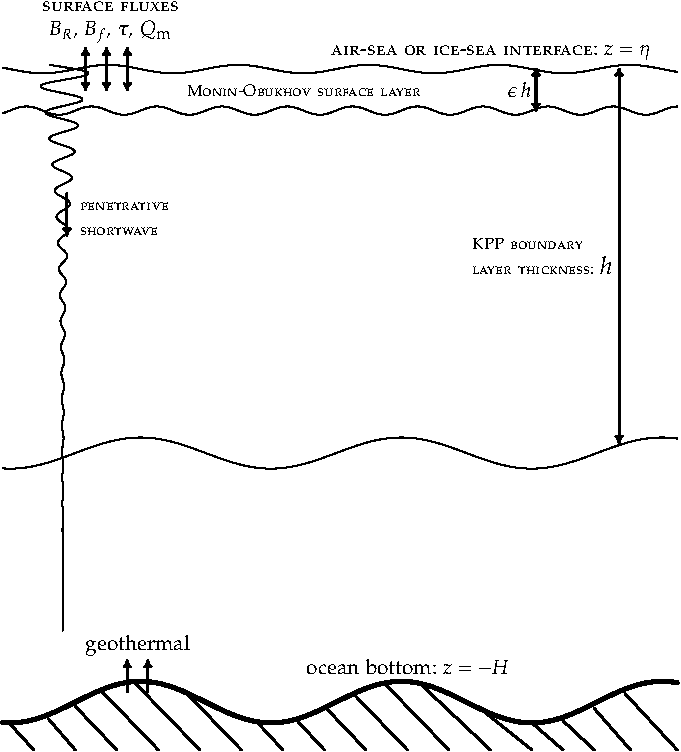
\includegraphics[angle=0,width=10cm,bb=0 0 327 361]{./mfpic_figs/cvmix_kpp_boundary_layer.pdf}
\caption[KPP boundary layer schematic]{\sf Schematic of the upper
  ocean boundary layer regions associated with the KPP boundary layer
  parameterization.  The upper ocean is exposed to non-penetrative
  air-sea and ice-sea fluxes of momentum $\bftau$ (Section
  \ref{section:boundary-forcing-momentum-kpp}), mass $\Qm$(Section
  \ref{section:boundary-forcing-buoyancy-kpp}), and buoyancy $B_{f}$
  (Section \ref{section:boundary-forcing-buoyancy-kpp}).  In addition,
  there is penetrative shortwave radiation, $-\overline{w \,
    \theta}_{R}$ (Section
  \ref{section:boundary-forcing-buoyancy-kpp}), indicated by the
  exponentially decaying vertical sinusoidal.  The Monin-Obukhov
  surface layer (Section \ref{section:m-o-similarity}) has a thickness
  $\epsilon \, h$, with $\epsilon \approx 0.1$.  The surface layer is
  where turbulence delivers fluxes to the molecular skin layer for
  transfer to the atmosphere or ice.  The surface layer starts from
  just beneath the surface roughness elements at the upper ocean
  interface.  Since neither these roughness elements, nor the
  molecular viscous sublayer, are resolved in ocean models, we assume
  in practice that the Monin-Obukhov surface layer extends to the sea
  surface at $z=\eta(x,y,t)$.  The KPP boundary layer includes the
  surface layer, and it has a thickness $h(x,y,t)$ determined by the
  KPP parameterization (Section \ref{subsection:kpp-obl-thickness}).
  The ocean bottom at $z=-H(x,y)$ is rigid and is exposed to
  geothermal heating.  Presently, the KPP boundary layer scheme has
  not been implemented in MOM or POP to parameterize bottom boundary
  layer physics, though nothing fundamental precludes such.  In fact,
  \cite{Durski_etal2004} provide just such an implementation.}
\label{fig:boundary-layer-schematic-kpp}
\end{center}
\end{figure}
%%%%%%%%%%%%%%%%%%%%%%%%%%%%%%%%%%%%%%%%%%%%%%%%%%%%%%%%%%%%%%%%%%%%%%%%



\subsubsection{Vertical turbulent velocity scale $w_{\lambda}$}

The velocity scale $w_{\lambda}$ is a function of depth within the
boundary layer, and a function of the field to which it refers. We
return to its specification in Section
\ref{subsection:vertical-velocity-scale}.


\subsubsection{Non-dimensional vertical shape function $G_{\lambda}(\sigma)$}

Non-dimensional vertical shape function $G_{\lambda}(\sigma)$ is used to
smoothly transition from the ocean surface to the bottom of the
boundary layer. \cite{LargeKPP} chose a cubic polynomial
\begin{equation}
 G_{\lambda}(\sigma) = a_{0} + a_{1} \, \sigma + a_{2} \, \sigma^{2} + a_{3} \, \sigma^{3}.
\label{eq:structure-function-gsigma}
\end{equation}
Since turbulent eddies do not cross the ocean surface at $\sigma=0$,
we should correspondingly have a vanishing diffusivity at $\sigma=0$.
This constraint is satisfied by setting 
\begin{equation}
 a_{0} = 0.
\end{equation}
We detail in Section \ref{subsection:kpp-shape-function} how to
specify the remaining expansion coefficients $a_{1}, a_{2}, a_{3}$.
In particular, we simplify the specification of \cite{LargeKPP}, with
their approach more complex than justified physically.


\subsection{The non-local transport $\gamma_{\lambda}$}
\label{subsection:kpp-nonlocal-transport-outline}

Section 2 of \cite{LargeKPP} notes the presence of many processes in
the boundary layer that lead to nonlocal transport.  This behaviour
leads to a diffusivity $K_{\lambda}$ that is a function of the surface
fluxes and boundary layer thickness $h$.  Furthermore, under
convective forcing (negative surface buoyancy forcing; $B_{f} < 0$),
fluxes can penetrate into stratified interior.  This characteristic
then motivates the introduction of a non-local transport term
$\gamma_{\lambda}$ to the KPP parameterization (equation
(\ref{eq:kpp-parameterization})) when $B_{f} < 0$.  To further
identify the need for a non-local transport term $\gamma_{\lambda}$,
we reproduce Figure 1 from \cite{LargeKPP}, here shown as Figure
\ref{fig:kpp-figure1-reproduced}.  The caption to Figure
\ref{fig:kpp-figure1-reproduced} explores the many facets of this
figure used to help justify the non-local term in KPP.  

%%%%%%%%%%%%%%%%%%%% %%%%%%%%%%%%%%%%%%%%%%%%%
\begin{figure}[h!t]
\begin{center}
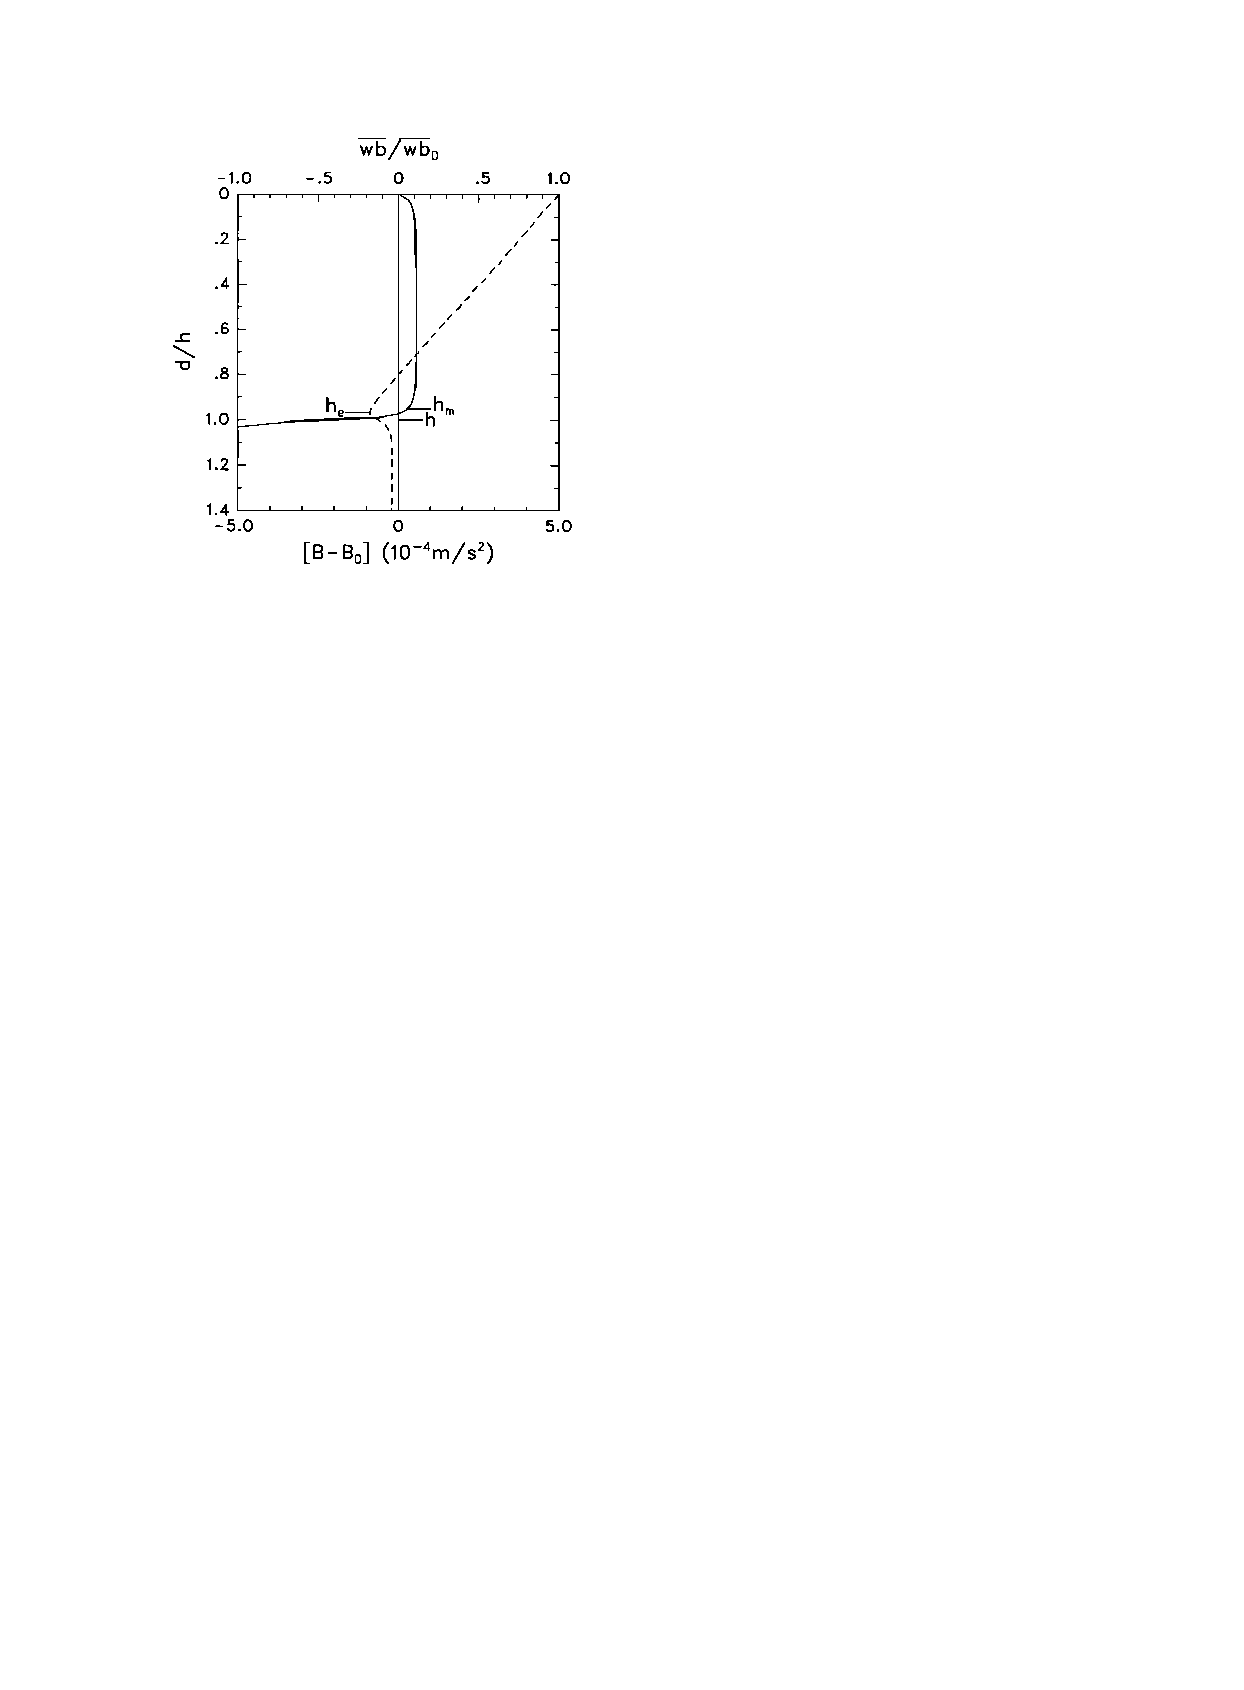
\includegraphics[angle=0,width=10cm,bb=44 530 310 758]{./figs/LargeKPP_fig1.pdf}
\caption[Figure 1 from \cite{LargeKPP}]{
  \sf
This is a reproduction of
  Figure 1 from \cite{LargeKPP}.
  The figure is derived from a one-dimensional simulation after 3 days of
  convective deepening (zero winds; negative surface buoyancy forcing)
  into an initially uniformly  stratified water column.  The vertical axis
  is vertical distance starting from the ocean surface interface at
  $z=\eta$ and $d=0$, extending down to $d=h$ ($h=13.6$~m at this point
  of the integration), which is the base of
  the boundary layer, and finally to $d=1.4\, h$, which is beneath the
  boundary layer.

 \hspace{0.4cm} The horizontal axis on the bottom is the mean buoyancy, $B$,
  relative to that at the surface, $B_{0}$, and the profile is
  depicted by the solid line. Positive values of
  $B-B_{0}$ indicate that the mean buoyancy at a point is larger than 
  at the surface, with $B-B_{0} > 0$ expected under
  negative buoyancy forcing at the ocean surface.  

  \hspace{0.4cm}  The horizontal axis on
  the top is the ratio of the local turbulent buoyancy flux
  $\overline{w \, b}$ to the surface turbulent flux $\overline{w \,
    b}^{\eta}$ (denoted $\overline{w \, b}_{0}$ by \cite{LargeKPP}).
  The dashed line depicts this ratio.  Positive values of $\overline{w
    \, b}$ represent upward turbulent buoyancy fluxes; e.g., upward
  fluxes of heat for the case where buoyancy is determined by
  temperature, and the thermal expansion coefficient is positive.
  
  \hspace{0.4cm}  Positive values for $\overline{w \, b}$  in regions between roughly $0.35 < d
  < 0.8$ represent upward turbulent buoyancy fluxes in a region where the mean vertical
  gradient of $B$ is nearly zero, thus indicating non-local turbulent transport.
  In shallower regions with $d < 0.35$, the mean gradient is negative,
  $\partial_{z} B < 0$, and the fluxes are positive, $\overline{w \,
    b} > 0$, thus representing downgradient turbulent fluxes.
  Likewise, for $d> 0.8$, the turbulent fluxes are downgradient.

  \hspace{0.4cm} The mixed layer depth is denoted by $h_{m}$, though
  this depth is subject to arbitrary specification of the density
  difference. The entrainment depth is $h_{e}$, with this depth taken
  where the buoyancy flux reaches a negative extrema. Note that it is
  an empirical result that under pure convective forcing ($\bftau =0,
  B_{f} < 0$), the turbulent entrainment flux is roughly 20\% of the
  surface flux: $\overline{w \, b}^{d=h_{e}} = -\beta_{T} \;
  \overline{w \, b}^{d=0}$, where $\beta_{T} = 0.2$. This situation is
  depicted in the figure. }
\label{fig:kpp-figure1-reproduced}
\end{center}
\end{figure}
%%%%%%%%%%%%%%%%%%%%%%%%%%%%%%%%%%%%%%%%%%%%%%%%%%%%%%%%%%%%%%%%%%%%%%%%


As part of the KPP parameterization, the non-local transport,
$\gamma_{\lambda}$, aims to account for such processes as boundary
layer eddies whose transport may be unrelated to the local vertical
gradient of the mean field, and whose impacts may penetrate within the
stratified ocean interior. In general, \cite{LargeKPP} prescribe the
following characteristics to $\gamma_{\lambda}$.
\begin{itemize}

\item Page 371 of \citep{LargeKPP} notes that there is no theory for
  non-local momentum transport, and so the non-local transport
  directly affects only the tracer fields:
\begin{equation}
 \gamma_{\lambda} \; \; = \; \; 
\left\{
 \begin{array}{ll}
  0 \; \;  &\mbox{if $\lambda = (u,v,w)$ a velocity component}
 \\
  \ne 0 \; \; &\mbox{nonzero if $\lambda = \theta,s$ or another tracer.}
  \end{array}
 \right.
\end{equation}
However, \cite{Smyth_etal2002} consider a non-local term for momentum,
thus motivating further research to see whether it is suitable for
climate modeling.  

  \item The non-local transport is non-zero only within the OBL:  
\begin{equation}
 \gamma_{\lambda} \; \; = \; \; 
  \left\{ 
  \begin{array}{ll}
   0 \; \; &\mbox{if $\sigma > 1$}
   \\ 
   \ne 0  \; \; &\mbox{if $0 \le \sigma \le 1$.}
  \end{array}
 \right.
\end{equation}

  \item The non-local transport is non-zero only in the presence of
    destabilizing negative surface ocean buoyancy flux, whose presence
    gives rise to convective mixing:
\begin{equation}
 \gamma_{\lambda} \; \; = \; \; 
  \left\{ 
  \begin{array}{ll}
   0 \; \; &\mbox{for positive (stabilizing) surface buoyancy forcing}
   \\ 
   \ne 0  \; \; &\mbox{for negative (destabilizing) surface buoyancy forcing.}
  \end{array}
 \right.
\end{equation}

  \item The non-local transport can give rise, under
    certain conditions, to either down-gradient or up-gradient
    transport of the mean tracer field. Hence, it can either act to
    smooth gradients of mean fields (downgradient non-local fluxes) or
    enhance gradients (upgradient non-local fluxes).

\end{itemize}
In Section \ref{subsection:kpp-non-local-transport}, we provide to the
KPP parameterization of $\gamma_{\lambda}$.



\section{Surface ocean boundary momentum fluxes}
\label{section:boundary-forcing-momentum-kpp}

In this section and Section
\ref{section:boundary-forcing-buoyancy-kpp}, we present features of
how surface boundary fluxes force the upper ocean, largely following
Appendix A of \cite{LargeKPP}.  The aim is to identify how surface
boundary fluxes impact the upper ocean, with this characterization
then used in Section \ref{section:m-o-similarity} to help establish
some basic features of ocean boundary layers.  These ideas are then
used in Section \ref{section:specifying-kpp-diffusivity-nonlocal} to
specify the diffusivity and non-local transport from the KPP
parameterization.

Vertical exchange of momentum across the atmosphere-ocean or
sea-ice-ocean boundary occurs largely through turbulent processes.
The resulting horizontal stress vector acting on the ocean, $\bftau$,
is determined through application of a bulk formula \citep[e.g., see
Appendix C of][]{CORE}. For our purposes, we assume $\bftau$ is given,
thus yielding the ocean kinematic fluxes associated with the turbulent
transport of momentum across the ocean surface
\begin{equation}
 -\overline{w \, {\bf u}}^{\eta} = \left( \frac{ \bftau }{\rho(\eta)} \right) \approx \left( \frac{ \bftau }{\rho_{0}} \right).
\label{eq:wu-kinematic-flux-kpp}
\end{equation} 
In this equation, $\rho(\eta)$ is the surface ocean density, which is
commonly approximated by the constant Boussinesq reference density
$\rho_{0}$.  A positive sign on a component of $\bftau$ acts to
accelerate the flow in the respective direction, whereas a positive
sign to a component of $\overline{w \, {\bf u}}^{\eta}$ removes
momentum from the ocean.  These sign conventions give rise to the
minus sign in the relation (\ref{eq:wu-kinematic-flux-kpp}).  In
addition to defining the kinematic surface fluxes, knowledge of
$\bftau$ allows us to compute surface boundary layer velocity scales
when working within the Monin-Obukhov similarity theory (Section
\ref{subsection:m-o-similarity-theory}).

In addition to turbulent momentum transfer, $\bftau$ is associated
with momentum transported through mass exchange across the ocean
surface, since water transported across the ocean generally carries a
nonzero momentum.  \cite{KanthaClaysonII} (see their page 431) point
out that this effect can be nontrivial, particularly when resolving
strong atmospheric storms. They also make the case for including this
effect in computing the Monin-Obukhov length scale defined by equation
(\ref{eq:m-o-length-scale})) (see their equation (4.3.11)).  Notably,
when running a coupled model, the stress from rain is included, since
it is part of the momentum convergence acting at the bottom of the
atmospheric column.  Modifying the stress from a prescribed
atmospheric state, such as CORE \citep{LargeYeager2009}, requires
further considerations.


\section{Surface ocean boundary buoyancy fluxes}
\label{section:boundary-forcing-buoyancy-kpp}

Turbulent and advective fluxes of momentum and buoyancy are
transferred across the upper ocean surface boundary, with ocean
processes such as advection and mixing then transporting the boundary
momentum and buoyancy laterally as well as into the ocean interior.
In contrast, penetrative shortwave radiation is absorbed into the
ocean absent ocean transport processes, with such absorption a
function of ocean optical properties.  In the unphysical case of
perfectly transparent seawater, shortwave radiation penetrates through
the boundary layer and so has no influence on boundary layer
processes.  In realistic cases, much of the shortwave radiation is
absorbed in the boundary layer, with only a fraction leaking through
to the interior. In general, such non-turbulent and non-advective
transport of buoyancy via penetrative radiation represents a
fundamentally novel aspect of ocean boundary layer physics relative to
the atmosphere.  Namely, for the atmosphere, radiative absorption is
far less relevant than in the upper ocean, since the atmosphere is
largely transparent to radiation.  We therefore consider penetrative
shortwave radiation as distinct from other buoyancy fluxes when
formulating how boundary fluxes impact the ocean.


\subsection{General features of buoyancy forcing}

The buoyancy of a fluid is commonly defined as (e.g., page 83 of
\cite{LargeKPP_lectures})
\begin{equation}
 B = g \, \left( \frac{ \rho_{0} - \rho}{\rho_{0}} \right), 
\label{eq:buoyancy-kpp}
\end{equation}
where $g$ is the constant gravitational acceleration, and $\rho_{0}$
is a reference density, taken here to equal the Boussinesq reference
density.  A reduction in density is associated with an increase in
buoyancy; that is, the water becomes more {\it buoyant}.  Changes in
buoyancy arise through changes in density associated with temperature
and salinity changes, since buoyancy changes are computed relative to
a fixed pressure level. In this way, buoyancy changes are directly
related to processes that impact locally referenced potential density.

Ocean buoyancy is affected through surface ocean heat, salt, and water
fluxes. 
\begin{itemize}

\item Turbulent processes transfer heat through latent and sensible
  heating.

\item Longwave radiation cools the upper ocean, with this radiation
  affected by the upper ocean skin temperature.  

\item Penetrative shortwave radiation is absorbed in seawater.

\item The transfer of salt occurs when sea ice melts and forms.  This
  transfer is proportional to the water mass flux and the difference
  in salinity between the liquid ocean and sea ice.  More generally,
  we simply consider this to be a salt flux between sea ice and ocean,
  with this flux operationally computed as part of a sea ice model.

\item Advective processes transfer heat and salt across the ocean
  surface through the transfer of water mass across the interface.

\end{itemize}
  We further detail these fluxes in the following. 


\subsection{Temperature, salinity, and mass budget for a surface
  ocean model grid cell}

Buoyancy is not a prognostic variable in ocean models.  So to develop
a quantative understanding of how buoyancy is impacted by surface
fluxes, we consider the evolution of temperature, salinity, and mass
in an arbitrary top model grid cell, and focus exclusively on
evolution arising from surface boundary fluxes.  We write these
budgets in their finite volume sense as in MOM, which includes density
and thickness weighting
\begin{align}
 \partial_{t} \, (\rho \, \mathrm{d}z \, \Theta) &=  \Qm \, \Thetam 
  - Q_{\theta}^{\mbox{\tiny non-pen}} 
  + \left( Q_{\theta}^{\mbox{\tiny pen}}(z=\eta) - Q_{\theta}^{\mbox{\tiny pen}}(z=-\Delta z) 
     \right)
 \label{eq:surface-temperature-equation-kpp}
\\
 \partial_{t} \, (\rho \, \mathrm{d}z \, S) &=  \Qm \, \Sm - Q_{S}
 \label{eq:surface-salinity-equation-kpp}
  \\
 \partial_{t} \, (\rho \, \mathrm{d}z) &=
  \Qm.
 \label{eq:surface-mass-equation-kpp}
\end{align}
 We now detail the terms appearing in these equations.  
\begin{itemize}

\item $\rho \, \mathrm{d}z$ is the mass per horizontal area of
  seawater in the grid cell.  For a volume conserving Boussinesq
  fluid, $\rho$ is set to the constant reference density $\rho_{0}$.

\item $\Theta$ is the grid cell potential temperature, or more
  accurately it is the conservative temperature of
  \cite{McDougall2003}.

 \item $S$ is the grid cell salinity.

 \item $\Qm$ is the mass flux ($\mbox{kg} \, \mbox{m}^{-2} \,
 \mbox{sec}^{-1})$ of water crossing the ocean surface, with $\Qm >
 0$ for water entering the ocean (as when precipitation plus runoff
 exceeds evaporation).

\item $\Thetam$ is the temperature of water crossing the ocean
  surface, and $C_{p} \, \Qm \, \Thetam$ is the associated heat flux
  ($\mbox{W} \, \mbox{m}^{-2})$.  We further discuss this heat flux in
  Section \ref{subsection:advective-buoyancy-fluxes}.

\item $\Sm$ is the salinity of water crossing the ocean surface, and
  $\Qm \, \Sm$ is the associated mass flux.  Note that $\Sm$ is
  typically taken to be zero, as for precipitation and evaporation.
  However, rivers can contain a nonzero salt concentration, so we keep
  $\Sm$ for the following formulation.  We further discuss this salt
  flux in Section \ref{subsection:advective-buoyancy-fluxes}.

\item $C_{p}$ is the seawater heat capacity at constant pressure
  ($\mbox{J} \, \mbox{kg}^{-1} \, \mbox{}^{\circ}\mbox{C}^{-1}$).
  \cite{TEOS2010} provides the most precise value appropriate for an
  ocean with heat measured through conservative temperature.

\item $Q_{S}$ is the flux of salt ($\mbox{kg} \, \mbox{m}^{-2} \,
  \mbox{sec}^{-1})$ that leaves the ocean through the ocean surface.
  This flux arises in the transfer of salt when sea ice forms and
  melts.  We further discuss this salt flux in Section
  \ref{subsection:sea-ice-buoyancy-fluxes}.

\item $C_{p} \, Q_{\theta}^{\mbox{\tiny non-pen}}$ is the
  non-penetrative surface heat flux associated with turbulent
  processes (latent and sensible) and radiative longwave cooling
  ($\mbox{W} \, \mbox{m}^{-2}$).  The sign convention is chosen so
  that $Q_{\theta}^{\mbox{\tiny non-pen}} > 0$ for heat leaving the
  ocean surface (i.e., ocean cooling).  We further discuss this heat
  flux in Section \ref{subsection:non-pen-buoyancy-fluxes}.

\item $C_{p} \, Q_{\theta}^{\mbox{\tiny pen}}(z=\eta)$ is the
  radiative shortwave heat flux ($\mbox{W} \, \mbox{m}^{-2}$) entering
  the ocean through its surface at $z=\eta$, with
  $Q_{\theta}^{\mbox{\tiny pen}}(\eta) > 0$ warming the ocean surface.
  Likewise, $C_{p} \, Q_{\theta}^{\mbox{\tiny pen}}(z=-\Delta z)$ is
  the radiative shortwave heat flux leaving the top cell through its
  bottom face.  We further discuss this heat flux in Section
  \ref{subsection:pen-buoyancy-fluxes}.

\end{itemize}


\subsection{Salt fluxes from sea ice melt and formation} 
\label{subsection:sea-ice-buoyancy-fluxes}

The mass flux of salt $Q_{S}$ ($\mbox{kg} \, \mbox{m}^{-2} \,
\mbox{sec}^{-1})$ is positive for salt leaving the ocean surface.
There is transport of salt across the ocean surface when sea ice forms
and melts, due to the nonzero salt content in sea ice.  Otherwise, the
surface salt flux is generally zero for the large scale ocean. For
ocean models, however, the salt flux can be nonzero when formulating
the surface boundary in terms of virtual salt fluxes rather than real
water fluxes \citep{Huang1993,GriffiesPacSchmidtBalaji2001}.  This
formulation is not recommended, as it is distinctly unphysical and
unnatural, particularly when using an explicit free surface or bottom
pressure.


\subsection{Salt and heat fluxes associated with water transport} 
\label{subsection:advective-buoyancy-fluxes}

In most cases, salinity in the water fluxed across the ocean surface
is zero, so that $\Sm=0$.  However, there are some cases where rivers
have a nonzero salinity so that $\Sm \ne 0$ and the product $\Qm \,
\Sm$ leads to an advective transport of salt across the ocean surface.

Since water transported across the ocean has a nonzero heat content,
this transport in turn affects the net heat content in the upper
ocean.  One can either prescribe the temperature of this water,
$\Thetam$, or the product $\Qm \, \Thetam$.  Consider the case where
the product is specified for river water entering the ocean, which is
the case with the GFDL land model used in the earth system model of
\cite{Dunne_etal_part1_2012}.  In this case, the heat flux with
respect to $0^{\circ}C$ (in units of $\mbox{W}~\mbox{m}^{-2}$) of
liquid river runoff ${\cal H}^{\mbox{\tiny liquid runoff}}$ is given
to the ocean from the land model, so that
\begin{equation}
     \Qm \, \Thetam = \frac{  {\cal H}^{\mbox{\tiny liquid runoff}} } {C_{p}^{\mbox{\tiny liquid runoff}}},
\label{eq:river-heating-kpp}
\end{equation}
with $C_{p}^{\mbox{\tiny liquid runoff}}$ the heat capacity of the
water coming in from the river runoff.  Likewise, if the heat
associated with frozen runoff (e.g., calving land ice) is provided by
the land model, then we have
\begin{equation}
      \Qm \, \Thetam = \frac{{\cal H}^{\mbox{\tiny solid runoff}}}{C_{p}^{\mbox{\tiny solid runoff}}},
\end{equation}
with $C_{p}^{\mbox{\tiny solid runoff}}$ the heat capacity of the
solid runoff.  These two heat capacities are typically provided by the
component model (i.e., the land model) used to compute the runoff
fields.  Similar considerations hold for transfer of water betwen sea
ice models and the ocean.


\subsection{Non-penetrative surface heat fluxes} 
\label{subsection:non-pen-buoyancy-fluxes}

The heat flux $C_{p} \, Q_{\theta}^{\mbox{\tiny non-pen}}$ ($\mbox{W}
\, \mbox{m}^{-2}$) is defined with a sign so that it is positive for
heat leaving the ocean. This flux is comprised of the following
contributions \citep[see page 34 of][]{Gill1982}
\begin{equation}
 C_{p}  \, Q_{\theta}^{\mbox{\tiny non-pen}}
 =  Q_{\mbox{\scriptsize long}} + Q_{\mbox{\scriptsize latent}} +
     Q_{\mbox{\scriptsize sens}}. 
\label{eq:non-penetrative-for-kpp}
\end{equation}
Longwave, latent, and sensible heat fluxes are typically deposited or
withdrawn from the ocean surface layer (Section
\ref{section:m-o-similarity}).  In practice, ocean models assume
these fluxes are taken entirely from the surface grid cell.  

These fluxes are termed non-penetrative, since they are deposited or
withdrawn from the liquid ocean at a particular depth, generally the
top model grid cell.  Transport of the boundary buoyancy to another
depth occurs only through the action of ocean transport processes,
such as advection or mixing.  This behaviour contrasts to that of
penetrative shortwave radiation, which is transferred to depths as a
function of seawater optics, so does not depend on ocean transport.
We now comment in a bit more detail on the various non-penetrative
fluxes.

\subsubsection{Longwave radiation}

$Q_{\mbox{\scriptsize long}}$ is the longwave radiation leaving the
ocean in the form of the $\sigma_{\mbox{\tiny SB}} \, T^{4}$
Stefan-Boltzmann Law, with $T$ the skin temperature.
$Q_{\mbox{\scriptsize long}}$ is positive, thus cooling the ocean
surface.  There is, however, longwave heating that results from
cloud reflection of longwave cooling, thus tempering the cooling
impacts on the ocean.  



\subsubsection{Latent heat fluxes}

$Q_{\mbox{\scriptsize latent}}$ arises from phase changes whereby
liquid seawater either evaporates, or it acts to melt frozen
precipitation.  When seawater evaporates, the latent heat lost by the
ocean is determined by the latent heat of vaporization for fresh water
  \begin{equation}
  H^{\mbox{\tiny vapor}} = 2.5 \times 10^{6} \, \mbox{J} \, \mbox{kg}^{-1},
\end{equation}
so that 
\begin{equation}
  Q_{\mbox{\tiny evap}}  =  H^{\mbox{\tiny vapor}} \,  \Qm^{\mbox{\tiny evap}}
\end{equation}
where $\Qm^{\mbox{\tiny evap}}$ is the mass flux ($\mbox{kg} \,
\mbox{m}^{-2} \, \mbox{sec}^{-1})$ of fresh water leaving the ocean
due to evaporation. A similar expression holds when seawater melts
frozen precipitation (e.g., snow), in which case
\begin{equation}
  H^{\mbox{\tiny fusion}} = 3.34 \times 10^{5} \, \mbox{J} \, \mbox{kg}^{-1},
\end{equation}
 so that 
\begin{equation}
  Q_{\mbox{\tiny melt}}  =  H^{\mbox{\tiny fusion}} \,  \Qm^{\mbox{\tiny frozen precip}},
\end{equation}
where $\Qm^{\mbox{\tiny frozen precip}}$ is the mass flux ($\mbox{kg}
\, \mbox{m}^{-2} \, \mbox{sec}^{-1})$ of frozen precipitation falling
onto the ocean surface. Both $Q_{\mbox{\tiny evap}}$ and
$Q_{\mbox{\tiny melt}}$ are positive, indicating that they act to cool
the ocean.

\subsubsection{Sensible heat fluxes}

$Q_{\mbox{\tiny sens}}$ is the sensible heat transfer proportional to
the difference between atmosphere and ocean temperatures. Sensible
heating generally acts to cool the ocean, particularly near western
boundary currents such as the Gulf Stream, Kuroshio, and Agulhas.


\subsection{The case of frazil}
\label{subsection:frazil-and-kpp}

As the temperature of seawater cools to the freezing point, sea ice is
formed, initially through the production of frazil ice.  Frazil can
generally form at various levels in the upper ocean, though many ocean
models assume frazil production occurs just in the top grid cell.
Operationally in an ocean model, liquid water can be supercooled at
any particular time step through surface fluxes and transport.  An
adjustment process is used to heat the liquid water back to the
freezing point, with this positive heat flux $Q_{\mbox{\tiny frazil}}
> 0$ extracted from the ice model as frazil sea ice is formed.  When
that adjustment is performed may determine whether to include
$Q_{\mbox{\tiny frazil}}$ as part of the net heat flux impacting the
boundary layer turbulence.  We omitted frazil heating in equation
(\ref{eq:non-penetrative-for-kpp}), as that is the approach taken at
NCAR. However, others, such as GFDL prior to 2012, include frazil as
part of the KPP boundary layer calculation.  We summarize the issues
here.

\begin{itemize}

\item {\sc frazil omitted from $B_{f}$}: When computing $B_{f}$ for
  KPP, the NCAR practice omits frazil heating, as reflected in
  equation (\ref{eq:non-penetrative-for-kpp}).  In effect, this
  approach assumes that all the negative buoyancy forcing that occurs
  in the upper ocean is used to drive convective boundary layer
  turbulence. After mixing, a portion of the heat, $Q_{\mbox{\tiny
      frazil}} > 0$, is returned to the liquid ocean to warm the water
  back to freezing, with this heat taken from the ice model as it forms
  frazil sea ice.

\item {\sc frazil included in $B_{f}$}: Many ocean climate models
  compute frazil heating just in the top model grid cell.  It is thus
  operationally trivial to include $Q_{\mbox{\tiny frazil}} > 0$ as
  another term in the non-penetrative heating (equation
  (\ref{eq:non-penetrative-for-kpp})).  Physically, this approach adds
  the amount of heat $Q_{\mbox{\tiny frazil}}$ to the buoyancy flux,
  and so potentially reduces the strength of the otherwise convective
  turbulence in the upper ocean.  This approach has been used at GFDL
  prior to 2012.

\end{itemize}
We have no strong argument for one approach versus the other.  Tests
should be run to consider sensitivity to the choice.



\subsection{Penetrative shortwave heating} 
\label{subsection:pen-buoyancy-fluxes}

The penetrative shortwave radiative heat flux $C_{p} \,
Q_{\theta}^{\mbox{\tiny pen}} > 0$ arises from the net shortwave
radiation entering through the ocean surface and absorbed by seawater.
This heat flux does {\it not} arise from turbulent or advective
processes, which makes it distinct from other heat and salt fluxes
impacting the ocean through its upper boundary.  This radiation is not
generally deposited entirely within the ocean surface layer or the top
ocean model grid cell. Instead, a fraction of this radiation can
penetrate to beneath the surface ocean grid cell, with the fraction
depending on the optical properties of seawater.  Hence, we subtract a
heat flux $C_{p} \, Q_{\theta}^{\mbox{\tiny pen}}(z=-\Delta z)$, which
represents the radiative shortwave heat flux passing through the
bottom of the surface ocean cell at $z=-\Delta z$.  It is the
difference,
\begin{equation}
   \mbox{net shortwave heating of surface grid cell} = 
  C_{p} \, \left( Q_{\theta}^{\mbox{\tiny pen}}(z=\eta) 
                    -Q_{\theta}^{\mbox{\tiny pen}}(z=-\Delta z) \right)
\end{equation}
that stays in the surface grid cell.  When considering the same budget
for the surface ocean boundary layer, we are interested in the
shortwave flux that penetrates through the bottom of the boundary
layer at $z=-h$.


\subsection{Buoyancy budget for a surface ocean model grid cell}

We now bring the previous fluxes together to form the budget for
buoyancy in a surface grid cell due to the impacts of surface fluxes.
The resulting expression is then used to derive an expression for the
buoyancy forcing that acts on the ocean surface boundary layer.
Buoyancy (equation (\ref{eq:buoyancy-kpp})) has a time tendency given
by
\begin{equation}
 -\left( \frac{\rho_{0}}{g} \right) \,  \frac{\partial B}{\partial t} 
  =  \rho_{,\Theta} \, \frac{\partial \Theta}{\partial t}  + \rho_{,S} \, \frac{\partial S}{\partial t},
\label{eq:buoyancy-time-tendency-kpp}
\end{equation}
 where we introduced the shorthand notation 
\begin{align}
\rho_{,\Theta} &=
 \left( \frac{\partial \rho}{\partial \Theta} \right)_{S,p} 
\\
\rho_{,S} &=
 \left( \frac{\partial \rho}{\partial S} \right)_{\Theta,p} 
\end{align}
for the partial derivatives of density with respect to conservative
temperature and salinity, respectively, each with pressure held
constant.  We wish to form an evolution equation for buoyancy at the
ocean surface grid cell just due to the effects of surface forcing.
For this purpose, multiply the temperature equation
(\ref{eq:surface-temperature-equation-kpp}) by $\rho_{,\Theta}$ and
add to the surface salinity equation
(\ref{eq:surface-salinity-equation-kpp}) multiplied by $\rho_{,S}$
\begin{equation}
  \rho_{,\Theta} \, (\rho \, \mathrm{d}z \, \Theta)_{,t}
  +
  \rho_{,S}      \, (\rho \, \mathrm{d}z \, S)_{,t}
  =
  \Qm \, (\rho_{,\Theta} \, \Thetam +  \rho_{,S}  \, \Sm) 
  + \rho_{,\Theta} \, \left( 
     -Q_{\theta}^{\mbox{\tiny non-pen}} + 
    \delta_{k} \, Q_{\theta}^{\mbox{\tiny pen}} \right)
  -  \rho_{,S} \, Q_{S},
\end{equation}
 where we introduced the shorthand 
\begin{equation}
 \delta_{k} \, Q_{\theta}^{\mbox{\tiny pen}} = 
   Q_{\theta}^{\mbox{\tiny pen}}(z=\eta) - Q_{\theta}^{\mbox{\tiny pen}}(z=-\Delta z).
\end{equation}
We now use the mass budget (\ref{eq:surface-mass-equation-kpp}) and
introduce the buoyancy tendency according to equation
(\ref{eq:buoyancy-time-tendency-kpp}) to realize an expression for the
time tendency of the surface ocean buoyancy
\begin{equation}
  (\rho_{0}/g) \, \rho \, \mathrm{d}z \, \left( \frac{\partial B}{\partial t} \right)
  =
  \Qm \, \left[  \rho_{,\Theta} \, (\Theta - \Thetam)  
                   + \rho_{,S} \, (S - \Sm) \right]
+ \rho_{,\Theta} \, \left( Q_{\theta}^{\mbox{\tiny non-pen}} - \delta_{k} \, Q_{\theta}^{\mbox{\tiny pen}} \right)  
+ \rho_{,S} \, Q_{S}.
\end{equation}
Now introduce the thermal expansion and saline contraction
coefficients
\begin{align}
 \alpha &= -\frac{1}{\rho} \, \left( \frac{\partial \rho}{\partial \Theta} \right)_{S,p} 
\label{eq:alpha-kpp}
\\
\beta &= \frac{1}{\rho} \, \left( \frac{\partial \rho}{\partial S} \right)_{\Theta,p}
\label{eq:beta-kpp}
\end{align}
to render 
\begin{equation}
 \mathrm{d}z \, \left( \frac{\partial B}{\partial t} \right)
  =
 \frac{g}{\rho_{0}} \left( 
 \Qm \, \left[ -\alpha \, (\Theta - \Thetam) +  \beta \, (S - \Sm) \right]
 + \alpha \, ( \delta_{k} \, Q_{\theta}^{\mbox{\tiny pen}} - Q_{\theta}^{\mbox{\tiny non-pen}} )
 + \beta \, Q_{S} \right). 
\label{eq:buoyancy-tendency-top-cell}
\end{equation}


\subsection{Surface boundary terms contributing to ocean buoyancy
  evolution}

We now summarize the various surface boundary terms appearing on the
right hand side of the surface buoyancy budget
(\ref{eq:buoyancy-tendency-top-cell}).


\subsubsection{Heat carried by water transport}

Assuming a positive thermal expansion coefficient, $\alpha > 0$, the
term $-\Qm \, \alpha \, (\Theta - \Thetam)$ reduces ocean buoyancy
when adding water $\Qm > 0$ to the ocean that is colder than the
surface ocean temperature, $\Theta = \Theta_{k=1}$.  The opposite
occurs in regions of cold fresh waters, such as the Baltic, where
$\alpha < 0$.  In such cases, adding water to the ocean that is colder
than the sea surface temperature increases seawater buoyancy.  We now
consider in turn the three cases evaporation, precipitation, and
liquid river runoff and indicate how they are typically treated in
climate models.

  \begin{itemize}

  \item It is quite accurate to assume that evaporating water leaves
    the ocean at the sea surface temperature, so that
\begin{equation}
   \Theta^{\mbox{\tiny evap}} = \Theta_{k=1},
\end{equation}
in which case there is no change to ocean buoyancy upon transfer of
evaporating water across the ocean surface.  This is the approach
taken by all ocean climate models.

\item Precipitating liquid water need not fall on the ocean at the sea
  surface temperature, so that
\begin{equation}
   \Theta^{\mbox{\tiny precip}} \ne \Theta_{k=1} \qquad \mbox{real world}.
\end{equation}
\cite{KanthaClaysonII} (see their page 429) discuss this difference,
and the associated transfer of heat across the ocean due to rain
events, particularly in the West Pacific.  However, we know of no
climate modeling application in which the atmospheric model component
carries information about the temperature of its condensed water, nor
the heat content of that water.  Hence, operationally all climate
modeling applications assume that
\begin{equation}
   \Theta^{\mbox{\tiny precip}} = \Theta_{k=1} \qquad \mbox{climate models},
\end{equation}
in which case there is no change in ocean buoyancy upon transfer of
precipitating liquid water across the ocean surface.  

\item Realistic river models carry the heat content of river water and
  pass this content to the ocean model at river mouths.  Following
  from the discussion surrounding equation
  (\ref{eq:river-heating-kpp}), we may thus write the river
  contribution to the buoyancy budget in the form
\begin{equation}
 -\Qm \, \alpha \, (\Theta - \Thetam) = \alpha \, \left(
  -\Qm \, \Theta  + \frac{  {\cal H}^{\mbox{\tiny liquid runoff}} }  {C_{p}^{\mbox{\tiny liquid runoff}}} \right).
\end{equation}
Depending on the heat content of liquid runoff relative to the sea
surface, ocean buoyancy may increase or decrease when liquid runoff
enters the ocean.

\end{itemize}

\subsubsection{Salt carried by water transport}

The haline contraction coefficient, $\beta$, is generally positive.
Hence, the term $\Qm \, \beta \, (S - \Sm)$ increases ocean buoyancy
for those cases where the sea surface salinity, $S_{k=1}$, is greater
than the salinity of the water transferred across the ocean surface.
Most applications assume $\Sm = 0$, such as for evaporation and
precipitation
\begin{align}
 S^{\mbox{\tiny evap}} &= 0 
\\
 S^{\mbox{\tiny precip}} &= 0.
\end{align}
 However, river models sometimes consider a nonzero salinity of the
 runoff, in which case 
\begin{equation}
 S^{\mbox{\tiny liquid runoff}} \ne 0. 
\end{equation}


\subsubsection{Penetrative radiation}

Shortwave radiation is absorbed by seawater as it penetrates from the
surface into the upper ocean. Hence, $\delta_{k} \,
Q_{\theta}^{\mbox{\tiny pen}} > 0$ so that radiation increases the
grid cell buoyancy.


\subsubsection{Non-penetrative heating}

Longwave, latent, and sensible heating generally cool the upper ocean,
and so lead to a decrease in ocean buoyancy for regions where the
thermal expansion coefficient, $\alpha$, is positive.  In those few
regions where $\alpha < 0$, such as the Baltic, non-penetrative
cooling can stabilize the column.


\subsubsection{Salt fluxes due to sea ice melt or formation}

Salt is exchanged with the ocean when sea ice melts and forms, so that
the term $\beta \, Q_{S}$ can either increase (when salt is removed
from the liquid ocean) or decrease (when salt is added to the liquid
ocean) buoyancy.


\subsection{Buoyancy forcing that acts on the OBL}
\label{subsection:buoyancy-forcing-obl}

The expression (\ref{eq:buoyancy-tendency-top-cell}) for the buoyancy
forcing from surface fluxes acting on a surface grid cell is now
extended to an expression for the buoyancy forcing on the OBL.  The
only subtle point concerns the treatment of penetrative shortwave
radiation.  Rather than consider that radiation leaving the bottom of
the surface cell at $z=-\Delta z$, we are now concerned with that
leaving the bottom of the boundary layer at $z=-h$.  We also multiply
this penetrative flux by the thermal expansion coefficient at that
depth, rather than the expansion coefficient in the ocean surface
cell.  In this way we write the buoyancy forcing acting on the
boundary layer
\begin{equation}
B_{f} =  \frac{g}{\rho_{0}} 
  \left[ 
 \Qm \, [ -\alpha \, (\Theta - \Thetam) +  \beta \, (S - \Sm) ]
  -\alpha \,  Q_{\theta}^{\mbox{\tiny non-pen}} + \beta \, Q_{S} 
  \right]
+ \left[ 
    \left( \alpha \, Q_{\theta}^{\mbox{\tiny pen}} \right)_{z=\eta}
 - \left( \alpha \, Q_{\theta}^{\mbox{\tiny pen}} \right)_{z=-h}
 \right].
\label{eq:buoyancy-forcing-obl}
\end{equation}
This expression for the net buoyancy forcing acting on the boundary
layer can be written as the sum of two terms
\begin{equation}
 B_{f} =  -\overline{w \, b}^{\eta}  + B_{R}. 
\label{eq:buoyancy-forcing-kpp}
\end{equation}
The first term takes the form of a kinematic turbulent flux at the
ocean surface
\begin{equation}
 -\overline{w \, b}^{\eta} =  
  \frac{g}{\rho_{0}} 
  \left[ 
 \Qm \, [ -\alpha \, (\Theta - \Thetam) +  \beta \, (S - \Sm) ]
  -\alpha \,  Q_{\theta}^{\mbox{\tiny non-pen}} + \beta \, Q_{S} 
 \right],
\label{eq:surface-turbulent-kinematic-flux}
\end{equation}
where the minus sign on the left hand side accounts for the assumption
that $w > 0$ for upward velocity.  The second term accounts for the
penetrative radiation, which is neither a turbulent flux nor advective
flux
\begin{equation}
 B_{R} = \left( \alpha \, Q_{\theta}^{\mbox{\tiny pen}} \right)_{z=\eta}
          -\left( \alpha \, Q_{\theta}^{\mbox{\tiny pen}} \right)_{z=-h}.
\label{eq:penetrative-buoyancy-kpp}
\end{equation}
The corresponding heat flux convergence onto the boundary layer is
given by (see equation (A4) of \cite{LargeKPP})
\begin{equation}
 Q_{R} = \left(Q_{\theta}^{\mbox{\tiny pen}} \right)_{z=\eta}
          -\left(Q_{\theta}^{\mbox{\tiny pen}} \right)_{z=-h}.
\label{eq:penetrative-heating-kpp}
\end{equation}
Notably, $B_{R}$, and hence $B_{f}$, are two-dimensional functions of
the boundary forcing, even though they depend on the depth to which
the penetrative radiation extends.


\section{Surface layer and Monin-Obukhov similarity}
\label{section:m-o-similarity}

The semi-empirical Monin-Obukhov similarity theory has proven quite
useful in describing general features of boundary layer turbulence
active in the atmospheric planetary boundary layer \citep[see, e.g.,
Section 3.3 of][]{KanthaClaysonII}. One may thus choose to apply these
ideas to the ocean planetary boundary layer, particularly since the
atmospheric boundary layer is far better measured than the ocean, and
there are certain features that are similar. However, before applying
the Monin-Obukhov similarity theory to the ocean, we acknowledge some
characteristics of the ocean surface boundary layer that distinguish
it from atmospheric boundary layers.

\begin{itemize}

\item Surface ocean gravity waves can impact a nontrivial fraction of
  the ocean surface boundary layer, whereas such waves only impact a
  small fraction of atmospheric boundary layers.

\item The surface ocean velocity is generally the largest velocity in
  the ocean. In contrast, the surface atmospheric velocity vanishes
  over land and is relatively small over the ocean.

\item The surface ocean absorbs shortwave solar radiation, whereas the
  atmosphere is nearly transparent to radiation.

\end{itemize}
Despite these basic distinctions between planetary boundary layers in
the atmosphere and ocean, \cite{LargeKPP} used the Monin-Obukhov
similarity theory to introduce scales for turbulent fluctuations and
to identify non-dimensional similarity functions in the ocean surface
layer.


\subsection{The surface layer}
\label{subsection:surface-layer}


A molecular layer exists within roughly a millimetre of the upper
ocean interface, with this layer dominated by molecular viscous and
diffusive effects \citep{LargeKPP_lectures}.  Since it is dominated by
molecular viscous effects, this layer is not turbulent and thus leads
to negligible mixing of tracer and momentum.  It is the molecular
layer that ultimately transfers properties between the ocean and
atmosphere or ice, including momentum and buoyancy.  The more this
layer is ``corrugated'' through wave breaking and other turbulent
action, the faster properties are transferred across the surface ocean
interface.

The ocean {\it surface layer} (Figure
\ref{fig:boundary-layer-schematic-kpp}) is a turbulent layer whose
turbulent fluxes are roughly independent of distance from the upper
boundary; i.e., the surface layer is nearly a {\it constant flux}
layer.  The surface layer starts just beneath the molecular viscous
layer.  Turbulence within the surface layer delivers properties to the
molecular layer for transfer to the atmosphere or ice
\citep{Fairall_etal1996}.  Given that no ocean model resolves the
molecular sublayer, the upper ocean interface at $z=\eta(x,y,t)$ in an
ocean model operationally starts at the top of the surface layer.


\subsection{Monin-Obukhov similarity theory}
\label{subsection:m-o-similarity-theory}

The surface turbulent layer is of fundamental importance for
determining the rate that properties are transferred across the
surface ocean interface.  It thus plays a key role in how the ocean is
forced.  If we needed to model all the details of this layer, then the
problem of coupled modeling would perhaps be intractable.
Fortunately, the Monin-Obukhov similarity theory has proven to be
quite useful in many contexts, particularly for the atmosphere
boundary layer.  Following \cite{LargeKPP}, we consider its use for
the ocean surface boundary layer.

Monin-Obukhov similarity theory assumes that the turbulent surface
layer is a constant flux layer that starts just beneath any roughness
elements, and certainly beneath the the molecular sublayer.  In the
absence of breaking surface waves, roughness elements arise from
capillary waves that allow the wind to affect the otherwise smooth
ocean surface, in which case the roughness length is on the order of
centimetres.  With breaking surface waves, the roughness length can
increase to the order of a metre \citep[e.g., see concluding section
to][]{Craig_Banner_1994}.  Furthermore, the scalings from
Monin-Obukhov are distinctly not correct with surface wave breaking
\citep[e.g.,][]{Craig_Banner_1994,Terray_etal1996}.  In the
formulation of \cite{LargeKPP}, surface gravity waves are ignored,
though we have more to say on surface waves in Section
\ref{section:surface-waves-and-kpp}.

Even if the surface layer is not a constant flux layer, the following
scalings are relevant so long as the surface fluxes remain the
dominant parameters determining properties of this layer
\citep{Tennekes1973}.  Within the surface layer, the relevant
dimensional quantities are the distance $d$ from the surface interface
at $z=\eta$, and the surface kinematic fluxes of momentum, tracer,
scalars, and buoyancy
\begin{align}
  \overline{w \, {\bf u}}^{\eta} &= \mbox{surface kinematic momentum flux}
\\
 \rho_{o} \, C_{p} \, \overline{w \, \theta}^{\eta} &= \mbox{surface kinematic heat flux}
\\
 \overline{w \, s}^{\eta} &= \mbox{surface kinematic scalar (e.g., salt) flux}
\\
 \overline{w \, b}^{\eta} &= \mbox{surface kinematic buoyancy flux.}
\end{align} 
 We now introduce the following dimensional scales.
\begin{itemize}

\item {\sc friction velocity}: From the surface kinematic momentum
  flux, we introduce the turbulent velocity scale, also known as the
  {\it friction velocity} scale
\begin{equation}
  u_{*}^{2} \equiv \left| \overline{w \, {\bf u}}^{\eta} \right|.
\end{equation}
Use of the identity (\ref{eq:wu-kinematic-flux-kpp}) provides a means
to compute the surface friction velocity given the surface momentum
stress
\begin{equation}
  \rho_{0} \, u_{*}^{2} = | \bftau |.
\label{eq:friction-velocity}
\end{equation}

\item {\sc temperature scale}: From the surface kinematic heat flux
  and the surface kinematic momentum flux, we define a scale for the
  surface turbulent temperature fluctuations
\begin{equation}
  \Theta_{*} = 
  -\left( 
   \frac{\overline{w \, \theta}^{\eta}}{  \sqrt { |\overline{w \, {\bf u}}^{\eta} | } }
   \right)
 = 
  -\left( 
   \frac{\overline{w \, \theta}^{\eta}}{  u_{*}}  \right).
\end{equation}
The sign is chosen so that turbulent fluxes leading to surface ocean
cooling, $\overline{w \, \theta}^{\eta} > 0$, correspond to a negative
turbulent temperature scale, $\Theta_{*} < 0$.

\item {\sc scalar scale}: From the surface kinematic scalar flux and
 the surface kinematic momentum flux, we define a scale for the
  surface turbulent scalar fluctuations
\begin{equation}
  S_{*} = 
  -\left( 
   \frac{\overline{w \, s}^{\eta}}{  u_{*}}  \right).
\label{eq:scalar-turbulent-scale-m-o}
\end{equation}

\item {\sc buoyancy scale}: From the surface kinematic buoyancy flux
  $-\overline{w \, b}^{\eta}$ (equation
  (\ref{eq:surface-turbulent-kinematic-flux})), and the penetrative
  buoyancy flux $B_{R}$ (equation (\ref{eq:penetrative-buoyancy-kpp}),
  we define a scale for the surface turbulent buoyancy fluctuations
\begin{equation}
  B_{*} = 
  \left( 
   \frac{B_{f} } {  u_{*} }
   \right)
 =
  \left( 
   \frac{-\overline{w \, b}^{\eta} + B_{R} } {  u_{*} }
   \right).
\end{equation}

\end{itemize}


\subsection{Similarity functions and length scale}
\label{subsection:m-o-similarity-functions}

The Monin-Obukhov similarity theory assumes the vertical gradient of
any mean field, $\Lambda$, within the surface turbulent layer is a
function of the scale $\Lambda_{*}$ of its turbulent fluctuations, the
buoyancy scale $B_{*}$, the velocity scale $u_{*}$, and the vertical
distance from the upper interface, $d=-z+\eta$ (equation
(\ref{eq:distance-from-surface})). In this case, we write
\begin{equation}
 \frac{\partial \Lambda}{\partial z} =  \Psi(d, u_{*}, B_{*}, \Lambda_{*}), 
\end{equation}
where $\Psi$ is an unknown function.  Although no exact analytical
expression exists for $\Psi$, Monin-Obukhov theory suggests that
progress can be made by fitting data to the following
form
\begin{equation}
  \frac{\partial \Lambda}{\partial z} = \left( \frac{\Lambda_{*}}{\kappa \, d} \right) \; \phi_{\Lambda}(\zeta).
\label{eq:m-o-similarity-form}
\end{equation}
In this expression, 
\begin{equation}
 \kappa \approx 0.4 
\end{equation}
is the von Karman constant, $\phi_{\Lambda}(\zeta)$ is a dimensionless
{\it similarity function} or flux profile that is dependent only on
the scaled distance
\begin{equation}
  \zeta \equiv \frac{d}{L},
\end{equation}
 and 
\begin{equation}
  L = \frac{u_{*}^{2}}{\kappa \, B_{*}} = \frac{u_{*}^{3}}{\kappa \, B_{f}} 
  = \frac{ |\bftau/\rho_{0}|^{3/2}}{\kappa \, B_{f}}
\label{eq:m-o-length-scale}
\end{equation}
is the Monin-Obukhov length scale determined by the ratio of the
momentum forcing to buoyancy forcing.

The Monin-Obukhov length scale takes on the following values for the
suite of available boundary forcing
\begin{equation}
  L = \left\{ 
  \begin{array}{llll}
   0       &u_{*}=0, B_{*} \ne 0    &\bftau = 0, B_{f} \ne 0  &\mbox{zero winds}
  \\
   \infty &u_{*} \ne 0, B_{*}= 0  &\bftau \ne 0, B_{f} = 0 &\mbox{zero buoyancy forcing (neutral forcing)}
 \\
  >0     &u_{*} \ne 0, B_{*} > 0  &\bftau \ne 0, B_{f} > 0  &\mbox{stabilizing buoyancy forcing}
\\
  <0     &u_{*} \ne 0, B_{*} < 0  &\bftau \ne 0, B_{f} < 0 &\mbox{destabilizing or convective buoyancy forcing.}
\end{array}
 \right.
\end{equation}
Notably, $L$ is {\it not} the finite positive thickness of the surface
turbulent layer (Figure \ref{fig:boundary-layer-schematic-kpp}), as
evident since $L$ can be negative or infinite.  Instead, $L$ is the
depth scale at which buoyancy production of turbulent kinetic energy
is of the same magnitude as shear production.  For depths shallower
than $L>0$, shear production dominates due to the effects from
mechanical forcing through momentum stress $\bftau$. The case
$L=\infty$ is trivially dominated by shear production since there is
no buoyancy forcing.  For depths deeper than $L$, buoyancy production
dominates the turbulence.  The case of $L < 0$ (convection) is always
dominated by buoyancy production.

The similarity function $\phi_{\Lambda}$ appearing in equation
(\ref{eq:m-o-similarity-form}) satisfies the following limit case
under neutral forcing (zero buoyancy forcing)
\begin{equation}
  \phi_{\Lambda}(0) = 1 \qquad \mbox{arising from $B_{f} = 0$ so that $L=\infty$ and $\zeta = d/L = 0$.} 
\end{equation}
This limit reduces the more general Monin-Obukhov form for the
vertical derivative (\ref{eq:m-o-similarity-form}) to the logarithmic
Law of the Wall form 
\begin{equation}
     \frac{\partial \Lambda}{\partial z} = \left(
    \frac{\Lambda_{*}}{\kappa \, d} \right)  \qquad \mbox{neutral forcing so $\phi_{\Lambda}=1$.}
\label{eq:m-o-similarity-form-neutral}
\end{equation}

In the general case of nonzero buoyancy forcing, we integrate the
similarity form (\ref{eq:m-o-similarity-form}) to expose the
logrithmic Law of the Wall for neutral forcing, plus a term present
with nonzero buoyancy forcing.  For this purpose, rewrite equation
(\ref{eq:m-o-similarity-form}) in terms of the scaled Monin-Obukhov
distance, $\zeta$, to have
\begin{equation}
  \frac{\partial \Lambda}{\partial \zeta} = -\left( \frac{\Lambda_{*}}{\kappa \, \zeta} \right) \; \phi_{\Lambda}(\zeta),
\label{eq:m-o-similarity-form-zeta}
\end{equation}
where we used the relation between vertical increments through
\begin{equation}
 \mathrm{d}\zeta = - L \, \mathrm{d}z
\label{eq:dzeta-change-variables}
\end{equation}
using $d=-z+\eta$ (equation (\ref{eq:distance-from-surface})).  We now
vertically integrate equation (\ref{eq:m-o-similarity-form-zeta}) to
have
\begin{equation}
 \Lambda(\zeta) = \Lambda(Z_{\lambda}/L)  
 +\left( \frac{\Lambda_{*}}{L} \right) \,
 \int\limits_{Z_{\lambda}/L}^{\zeta} \left(\frac{ (1-\phi_{\Lambda}) - 1}{\zeta'} \right) \, \mathrm{d}\zeta'.
\label{eq:intermediate-expression-mean-kpp}
\end{equation}
 In this expression, 
\begin{equation}
 Z_{\lambda} = \mbox{roughness length}
\end{equation}
introduced the roughness length associated with each fluctuating
field.  Within a distance $Z_{\lambda}$ or less from the boundary at
$z=\eta$, the kinematic fluxes are not expected to be constant due to
the impacts from roughness elements.  Hence, we expect the
Monin-Obukhov similarity theory to breakdown when getting closer than
the roughness length to the surface.

Integrating the right hand side of equation
(\ref{eq:intermediate-expression-mean-kpp}) from the roughness length
to an arbitrary point within the surface layer renders\footnote{The
  result (\ref{eq:general-expression-mean-m-o-similarity}) disagrees
  with equation (4) in \cite{LargeKPP} by a minus sign, with the
  origin of the minus sign the relation
  (\ref{eq:dzeta-change-variables}) between infinitesimal changes in
  $\zeta$ and infinitesimal changes in $z$.}
\begin{equation}
 \Lambda(\zeta) = \Lambda(Z_{\lambda}/L)   
 -\left( \frac{\Lambda_{*}}{L} \right) \, \ln(\zeta \, L/Z_{\lambda})
 +
  \left( \frac{\Lambda_{*}}{L} \right) \,
  \int\limits_{Z_{\lambda}/L}^{\zeta} \left(\frac{ (1-\phi_{\Lambda})}{\zeta'} \right) \, \mathrm{d}\zeta'.
\label{eq:general-expression-mean-m-o-similarity}
\end{equation}
As expected, the first term exposes the logarithmic Law of the Wall
behaviour occurring for neutral forcing conditions ($\phi_{\Lambda} =
1$).  Deviations from Law of the Wall for non-neutral forcing are
embodied in the integral on the right hand side.  Recall that values
$\zeta < Z_{\lambda}/L$ are within the roughness elements or molecular
sublayer, so the theory cannot be applied there.

\cite{LargeKPP} (see their page 365) use atmospheric boundary layer
results from \cite{Tennekes1973} to set the surface layer thickness to
(see Figure \ref{fig:boundary-layer-schematic-kpp})
\begin{equation}
 \epsilon = 0.1  \qquad \mbox{fraction of KPP boundary layer occupied by
   surface layer.}
\label{eq:epsilon-kpp}
\end{equation}
Within the surface layer, atmospheric boundary layer studies indicate
that turbulent fluxes are within 20\% of their surface values when
reaching a distance $d=\epsilon \, h$ from the upper ocean interface
at $d=0$.  The value of $\epsilon=0.1$ has never been observed in the
ocean, but there is no reason to believe it is fundamentally
incorrect. Hence, this is the value taken for the KPP scheme.


 
\section{Specifying the KPP parameterization}
\label{section:specifying-kpp-diffusivity-nonlocal}

We are now ready to determine the KPP boundary layer depth, $h$, the
diffusivity, $K_{\lambda}$, and non-local transport,
$\gamma_{\lambda}$, thus enabling a full parameterization of the
turbulent flux $\overline{w \, \lambda}$ according to
\begin{equation}
  \overline{w \, \lambda}= -K_{\lambda} \left( \frac{\partial \Lambda}{\partial z} - \gamma_{\lambda} \right),
\label{eq:kpp-parameterization-again}
\end{equation}
where the diffusivity is given by equation (\ref{eq:kpp-diffusivity}),
rewritten here as
\begin{equation}
 K_{\lambda}(\sigma) = h \, w_{\lambda}(\sigma) \, G_{\lambda}(\sigma).
\label{eq:kpp-diffusivity-again}
\end{equation}
Recall that 
\begin{equation}
  \sigma = d/h
\end{equation}
is the dimensionless distance from the upper surface normalized by the
boundary layer thickness, with
\begin{equation}
 d = -z + \eta
\end{equation}
 the dimensionful distance.  

\subsection{The turbulent vertical velocity scale $w_{\lambda}$} 
\label{subsection:vertical-velocity-scale}

We now determine the turbulent vertical velocity scale $w_{\lambda}$
appearing in equation (\ref{eq:kpp-diffusivity-again}). 


\subsubsection{Velocity scale with stable buoyancy forcing}

Following page 370 of \cite{LargeKPP}, we first specify the velocity
scale within the Monin-Obukhov surface layer, where $\sigma = d/h <
\epsilon = 0.1$.  We also assume stable buoyancy forcing, so that the
non-local term, $\gamma_{\lambda}$, vanishes.  We later extend these
results to the full boundary layer for arbitrary buoyancy forcing.

The similarity result (\ref{eq:m-o-similarity-form}) holds in the
surface layer, in which
\begin{equation}
  \frac{\partial \Lambda}{\partial z} = \left( \frac{\Lambda_{*}}{\kappa \, d} \right) \; \phi_{\Lambda}(\zeta).
\label{eq:m-o-similarity-form-again}
\end{equation}
We may eliminate the vertical gradient $\partial \Lambda/ \partial z$
using the KPP parameterization (\ref{eq:kpp-parameterization-again})
with a zero non-local term under stable buoyancy forcing
\begin{equation}
 \phi_{\Lambda} = -\frac{\kappa \, d}{\Lambda_{*}} \left( \frac{\overline{w \, \lambda}}{K_{\lambda}} \right).
\end{equation}
Substituting the turbulent scale $\Lambda_{*} =-\overline{w \,
  \lambda}^{\eta}/ u_{*}$ from equation
(\ref{eq:scalar-turbulent-scale-m-o}) yields
\begin{equation}
 K_{\lambda} \, \phi_{\Lambda} = \kappa \, d \, u_{*} \, \left( \frac{\overline{w \, \lambda}} {\overline{w \, \lambda}^{\eta} } \right).
\end{equation}
The KPP diffusivity expression (\ref{eq:kpp-diffusivity-again}) then
renders
\begin{equation}
 w_{\lambda}(\sigma) \, \sigma^{-1} \, G_{\lambda}(\sigma) = 
 \left(  \frac{\kappa \, u_{*}}{\phi_{\Lambda}(\sigma) }  \right) 
 \left( \frac{ \overline{w \, \lambda}^{\sigma}}{ \overline{w \, \lambda}^{\eta}}\right).
\end{equation}

Recalling that  $\sigma < \epsilon = 0.1$ in the surface
layer yields the approximate linear relation
\begin{equation}
\sigma^{-1} \, G_{\lambda}(\sigma)  \approx a_{1} + a_{2} \, \sigma,  
\end{equation}
where we used expression (\ref{eq:structure-function-gsigma}) for the
structure function $G_{\lambda}(\sigma)$.  Furthermore, within the
surface layer, turbulent fluxes for any fluctuating field,
$\overline{w \, \lambda}^{\sigma}$, are linearly proportional to their
surface value, $\overline{w \, \lambda}^{\eta}$.  We may thus use this
result to specify a part of the structure function according to
\begin{equation}
  a_{1} + a_{2} \, \sigma = \left( \frac{ \overline{w \, \lambda}^{\sigma}}{\overline{w \, \lambda}^{\eta}} \right).
\label{eq:specifying-structure-function}
\end{equation}
Note that as shown in Section \ref{subsection:kpp-shape-function},
there is generally a dependence of $a_{2}$ on the field $\lambda$,
whereas $a_{1}$ is unity for all fields.  With the specification
(\ref{eq:specifying-structure-function}), we are led to an expression
for the turbulent velocity scale within the surface layer
\begin{equation}
  w_{\lambda}(\sigma)  = \frac{\kappa \,  u_{*}}{\phi_{\Lambda}(\sigma  \, h/L)}   
 \qquad \mbox{for stable forcing $B_{f} > 0$ and $0 < \sigma < \epsilon$.}
\label{eq:wlambda-surface-layer}
\end{equation}
\cite{Troen_Mahrt1986} assume this expression is valid throughout the
stably forced boundary layer for $0 < \sigma < 1$, and \cite{LargeKPP}
also make that assumption.


\subsubsection{Velocity scale with unstable buoyancy forcing}

For unstable buoyancy forcing conditions, $B_{f} < 0$, the turbulent
velocity scales within the surface layer are assumed to be the same as
the stable velocity scale (\ref{eq:wlambda-surface-layer}), again
within the surface layer.  For unstable forcing beneath the surface
layer, $\epsilon < \sigma < 1$, \cite{LargeKPP} cap the velocity scale
to that evaluated at the base of the surface layer at $\sigma =
\epsilon$.  

\subsubsection{Summarizing properties of the turbulent velocity scale}

The net result for all conditions is that the turbulent vertical
velocity scale is given by
\begin{equation}
  w_{\lambda}(\sigma)  = \kappa \, u_{*} \, \left\{
 \begin{array}{llll}
   \phi^{-1}_{\Lambda}(\sigma \, h / L)   
  &\mbox{stable forcing $B_{f} > 0$} & \mbox{OBL}
  &\mbox{$0 < \sigma < 1$}
\\
  \phi^{-1}_{\Lambda}(\sigma \, h / L)   
  &\mbox{unstable forcing $B_{f} < 0$} &\mbox{surface layer}
  &\mbox{$\sigma <  \epsilon$}
\\
  \phi^{-1}_{\Lambda}(\epsilon \, h / L)   
 &\mbox{unstable forcing $B_{f} < 0$} &\mbox{OBL beneath surface layer}
 &\mbox{$\epsilon < \sigma < 1$.}
\end{array} 
 \right.
\label{eq:wlambda-general}
\end{equation}
We now summarize various properties of the velocity scale, with these
properties reflected in Figure \ref{fig:kpp-figure2-reproduced}.
\begin{itemize}

\item {\sc stable forcing}: The similarity functions
  $\phi_{\Lambda}$ and velocity scales $w_{\lambda}$ satisfy the
  following properties under positive buoyancy forcing, $B_{f}>0$.
 \begin{itemize}
 
 \item The similarity functions are increased so that the turbulent
   velocity scales are reduced.

 \item The similarity functions are the same for all scalars and
   momentum, so that the velocity scales $w_{\lambda}$ are the same.

\end{itemize}

\item {\sc neutral forcing}: with zero buoyancy forcing, $B_{f}=0$,
  the similarity functions satisfy $\phi_{\Lambda} = 1$, so that
  $w_{\lambda}(\sigma) = \kappa \, u_{*}$.

\item {\sc unstable forcing}: The similarity functions
  $\phi_{\Lambda}$ and velocity scales $w_{\lambda}$ satisfy the
  following properties under negative buoyancy forcing, $B_{f}<0$.
 \begin{itemize}

 \item The similarity functions $\phi_{\Lambda}$ are reduced so that
   the turbulent velocity scales $w_{\lambda}$ are enhanced.

 \item The similarity functions for momentum are larger than those for
   scalars, so that the velocity scales for momentum are smaller than
   for scalars: $w_{m} < w_{s}$.

 \item In the convective limit, for which $u_{*} \rightarrow 0$, the
   velocity scales behave according to 
\begin{equation}
 w_{\lambda} \sim w_{*} = (-B_{f} \, h)^{1/3}.
 \end{equation}
In order to satisfy this scaling, the similarity functions
$\phi_{\Lambda}$ must have the form 
\begin{equation}
  \phi_{\Lambda} = (a_{\lambda} - c_{\lambda} \, \zeta)^{-1/3}  \qquad \mbox{convective conditions with $u_{*} \rightarrow 0$,}
\label{eq:phi-under-convective-forcing}
\end{equation}
where $\zeta = d/L << 0$, and the constants $a_{\lambda}$ and
$c_{\lambda}$ are chosen to match the convective form
(\ref{eq:phi-under-convective-forcing}) to less unstable forms.  

We now use the expression (\ref{eq:phi-under-convective-forcing})
within the unstable surface layer ($\sigma < \epsilon$) form in
(\ref{eq:wlambda-general}) to render
\begin{equation}
\begin{split}
w_{\lambda} &= \kappa \, (a_{\lambda} \, u_{*}^{3} - c_{\lambda} \, u_{*}^{3} \, \zeta)^{1/3}
 \\
 &= \kappa \, [a_{\lambda} \, u_{*}^{3} - c_{\lambda} \, u_{*}^{3} \, (h\, \sigma/L) ]^{1/3}
 \\
 &= \kappa \, (a_{\lambda} \, u_{*}^{3} - c_{\lambda} \, \sigma \, \kappa \, h \, B_{f} )^{1/3}
\\
&= \kappa \, (a_{\lambda} \, u_{*}^{3} + c_{\lambda} \, \sigma \, \kappa \, w_{*}^{3} )^{1/3}
\\
 &\rightarrow 
  \kappa \, w_{*} \, (c_{\lambda} \, \sigma \, \kappa)^{1/3},
\end{split}
\end{equation}
where the final limit case is for the convective limit with $u_{*}
\rightarrow 0$.  Likewise, outside the surface layer ($\epsilon <
\sigma < 1$) we have
\begin{equation}
w_{\lambda} = \kappa \, (a_{\lambda} \, u_{*}^{3} + c_{\lambda} \, \epsilon \, \kappa \, w_{*}^{3} )^{1/3}
  \rightarrow 
  \kappa \, w_{*} \, (c_{\lambda} \, \epsilon \, \kappa)^{1/3},
\end{equation}
where again the final limit case is for the convective limit with
$u_{*} \rightarrow 0$.  

\end{itemize}

\end{itemize}




 
%%%%%%%%%%%%%%%%%%%% %%%%%%%%%%%%%%%%%%%%%%%%%
\begin{figure}[h!t]
\begin{center}
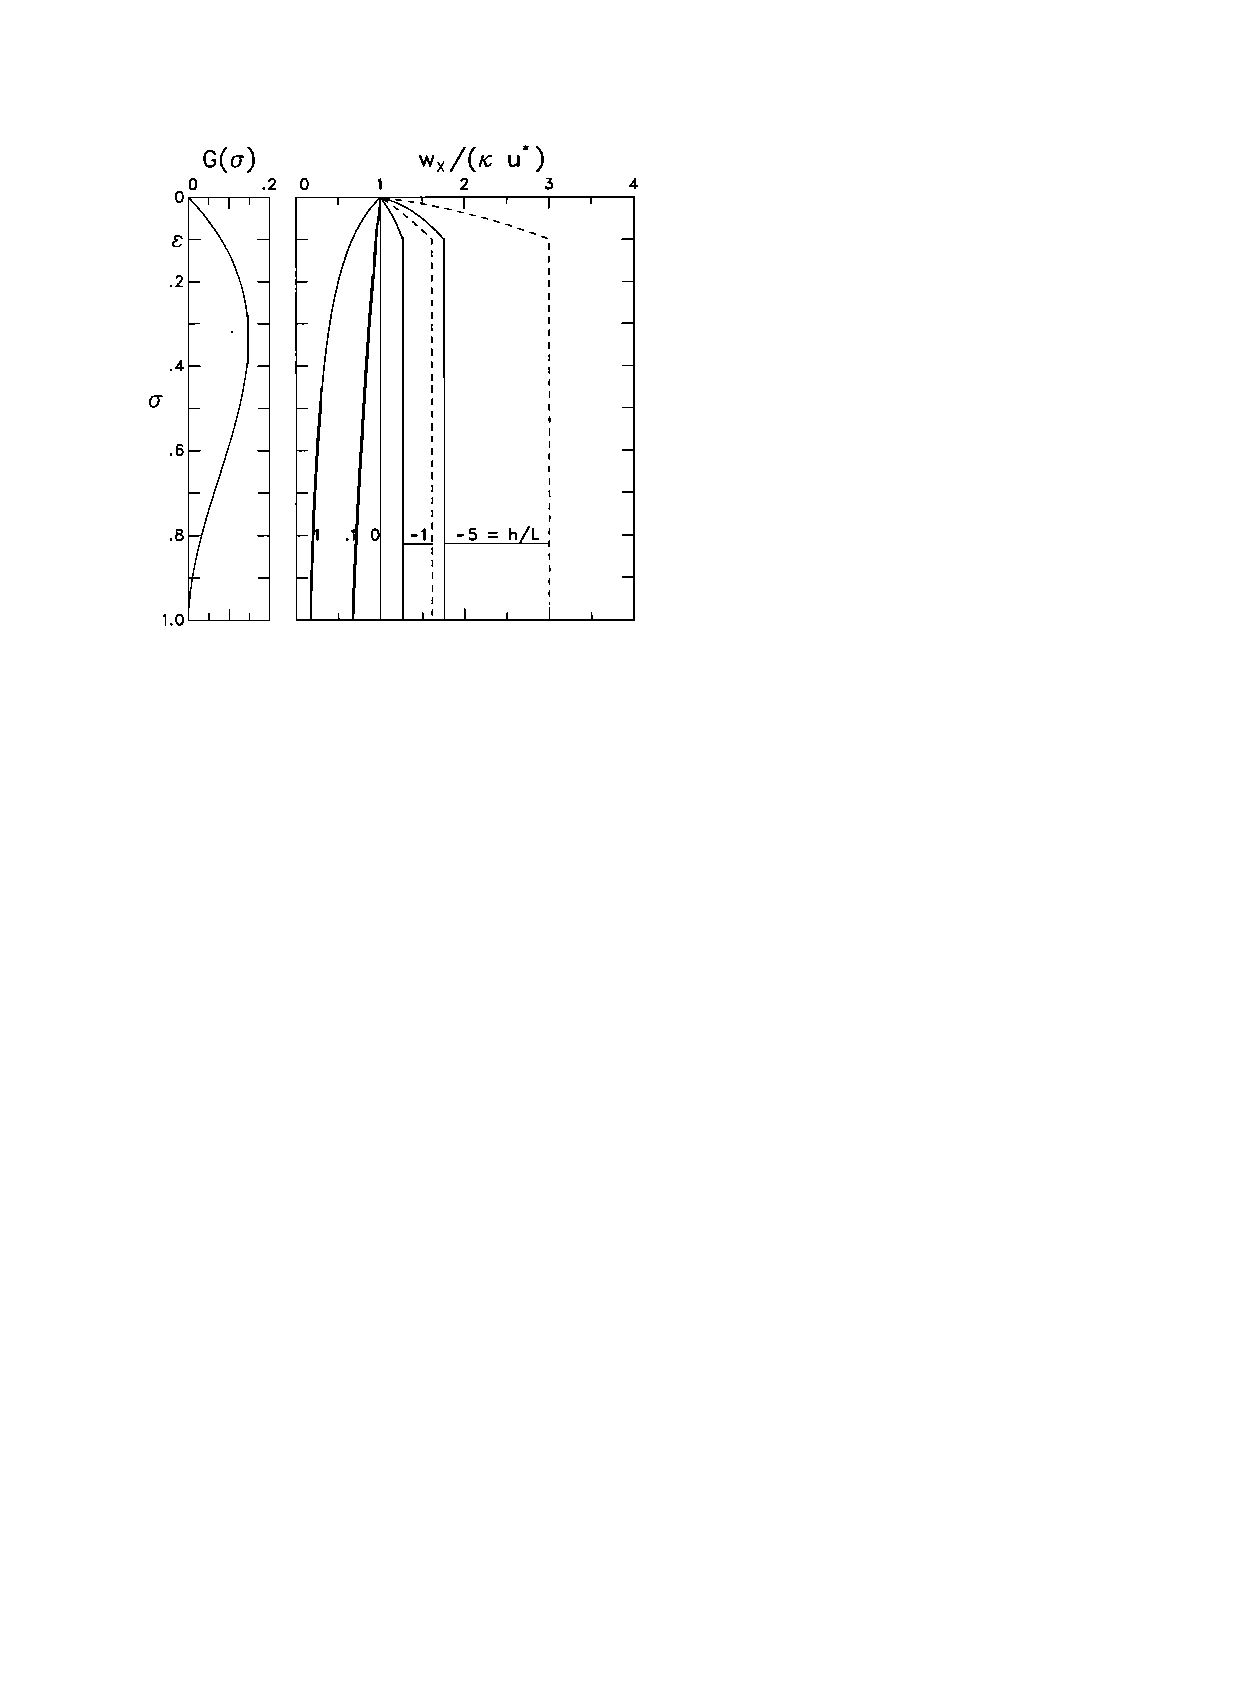
\includegraphics[angle=0,width=8cm,bb=62 503 310 747]{./figs/LargeKPP_fig2.pdf}
\caption[Figure 2 from \cite{LargeKPP}]{ \sf This is a reproduction of
  Figure 2 from \cite{LargeKPP}.  The vertical axis is the
  dimensionless vertical coordinate $\sigma = d/h$ within the KPP
  boundary layer $0 \le \sigma \le 1$.  The left panel shows the
  vertical profile of the shape or structure function,
  $G_{\lambda}(\sigma)$, used to scale the vertical diffusivity via
  equation (\ref{eq:kpp-diffusivity-again}).  The analytic form shown
  here is given by $G_{\lambda}(\sigma) = \sigma \, (1-\sigma)^{2}$,
  which corresponds to the \cite{Troen_Mahrt1986} form and which is
  independent of the quantity $\Lambda$ being diffused.
  \cite{LargeKPP} chose a more general form, based on the need to
  match boundary layer diffusivities to interior diffusivities in
  which case the shape function becomes a function of $\lambda$.  We
  detail this approach in Section \ref{subsection:kpp-shape-function}.
  The right panel shows various examples of the normalized turbulent
  velocity scale $w_{\lambda}$ (called $w_{x}$ in \cite{LargeKPP}),
  with the examples differing by the value of the dimensionless ratio
  $h/L$ between the boundary layer depth, $h$, and the Monin-Obukhov
  length scale $L$.  For unstable buoyancy forcing, $L<0$, the
  velocity scale for scalars, $w_{s}$ (dashed lines), is greater than
  that for momentum, $w_{m}$ (solid lines).  For stable forcing,
  $L>0$, and both scalar and momentum have the same turbulent velocity
  scales, $w_{s} = w_{m}$.  In general, the turbulent velocity scale
  is enhanced with unstable surface buoyancy forcing, and reduced with
  stable buoyancy forcing.}
\label{fig:kpp-figure2-reproduced}
\end{center}
\end{figure}
%%%%%%%%%%%%%%%%%%%%%%%%%%%%%%%%%%%%%%%%%%%%%%%%%%%%%%%%%%%%%%%%%%%%%%%%



\subsection{Similarity functions $\phi_{\Lambda}$}

The vertical velocity scales are functions of the similarity functions
$\phi_{\Lambda}$, also called the dimensionless flux profiles.
Appendix B of \cite{LargeKPP} present analytic forms for these
functions, based on fits to available data, with their Figure B1
(reproduced here as Figure \ref{fig:large-etal-figureB1}) providing a
summary of the choices for the momentum function $\phi_{m}$ and the
scalar function $\phi_{s}$.  Both functions agree for stable buoyancy
forcing, and they depend linearly on the dimensionless Monin-Obukhov
length $\zeta = d/L = \sigma \, h/L$.


\subsubsection{The \cite{LargeKPP} choices for unstable buoyancy forcing}

For unstable buoyancy forcing, where $L<0$ and so $\zeta < 0$, there
are two regimes.  The scalar function $\phi_{s}$ is always less than
the momentum function $\phi_{m}$.  Hence, for unstable forcing there
is a larger turbulent velocity scale for the scalars than momentum,
and thus a larger vertical diffusivity for scalars.  The turbulent
Prandtl number, $Pr$, is given by the ratio of the flux functions
\begin{equation}
  Pr = K_{m} / K_{s} = w_{m} / w_{s} = \phi_{m} / \phi_{s}.
\label{eq:prandtl-number}
\end{equation}
The choices made by \cite{LargeKPP} lead to a Prandtl number in the
convective limit ($\zeta \rightarrow -\infty$) of 
\begin{equation}
 Pr \rightarrow (c_{m}/c_{s})^{1/3} = 0.44,
\end{equation}
where $c_{m}$ and $c_{s}$ are parameters in the similarity functions
$\phi_{m}$ and $\phi_{s}$, respectively.

 
%%%%%%%%%%%%%%%%%%%% %%%%%%%%%%%%%%%%%%%%%%%%%
\begin{figure}[h!t]
\begin{center}
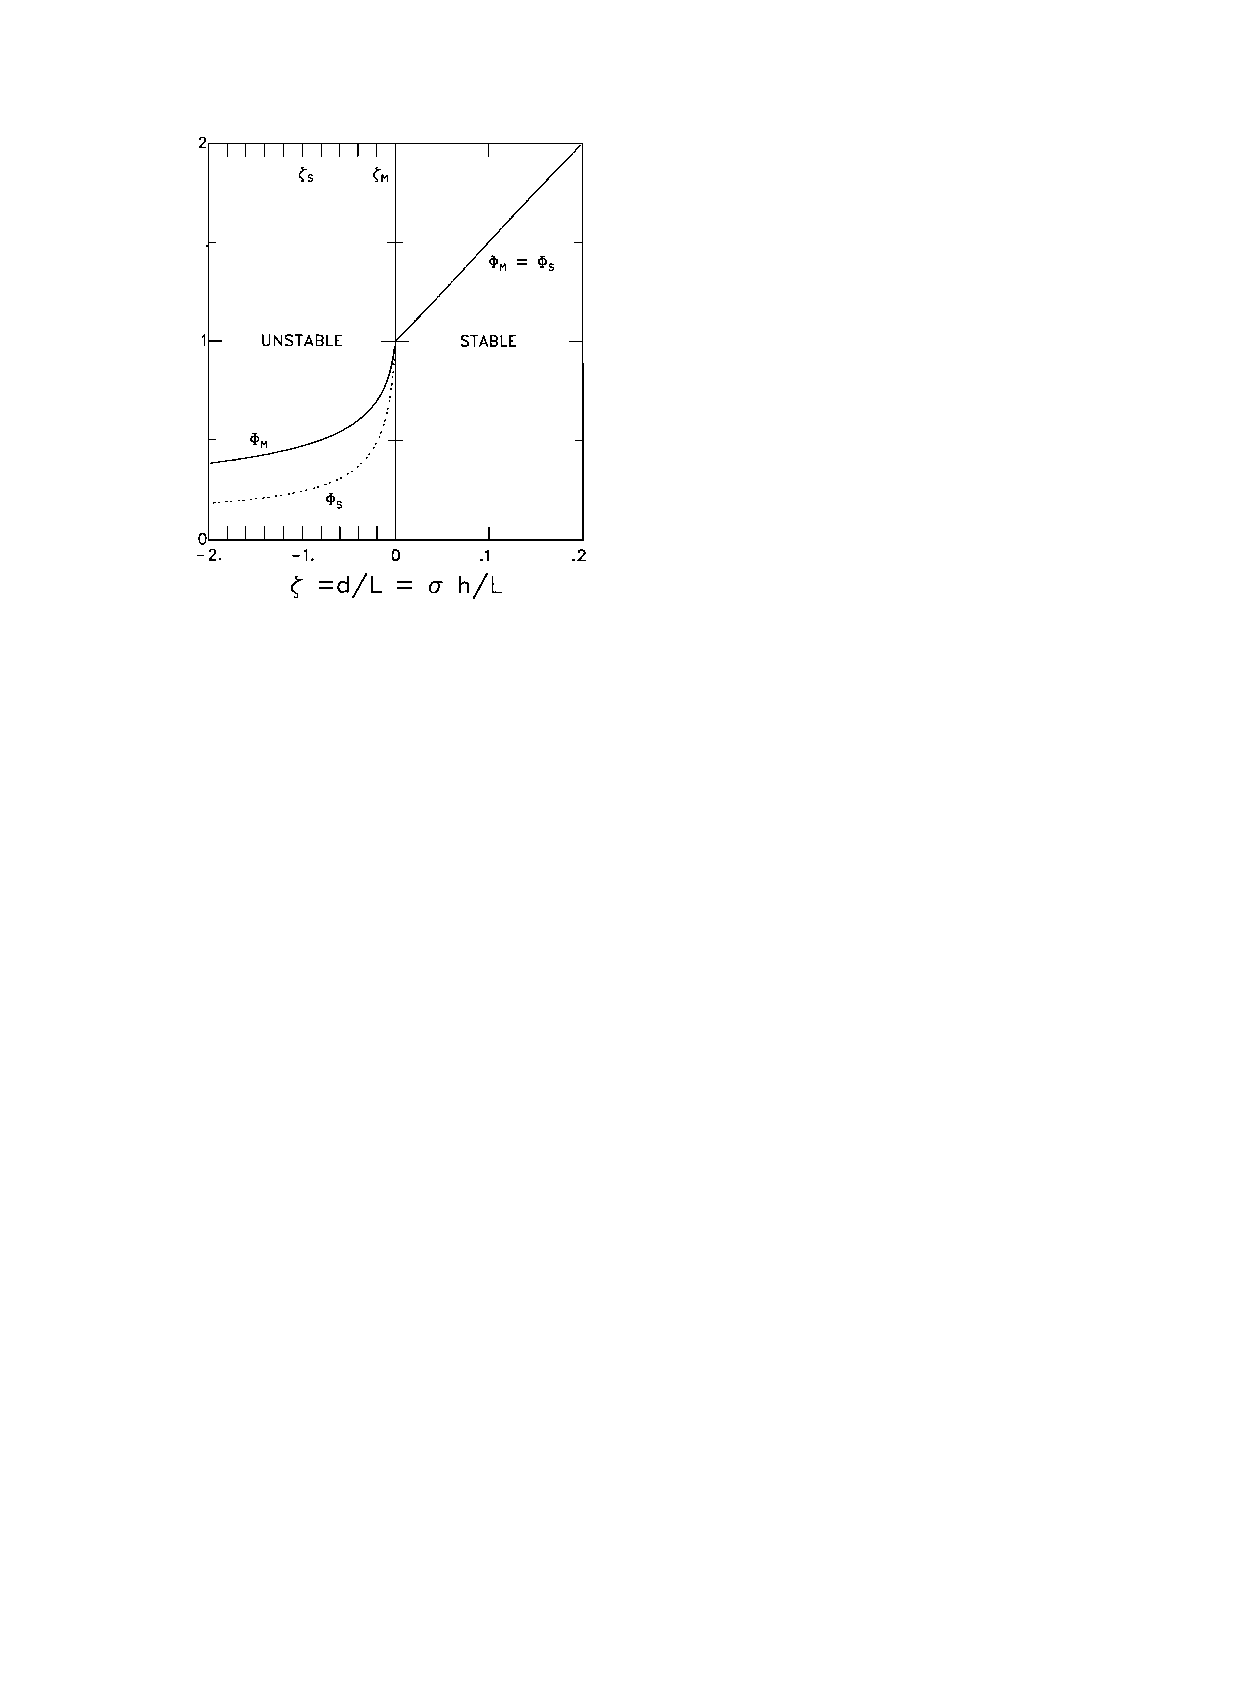
\includegraphics[angle=0,width=8cm,bb=89 521 292 747]{./figs/LargeKPP_figB1.pdf}
\caption[Figure B1 from \cite{LargeKPP}]{\sf This is a reproduction of
  Figure B1 from \cite{LargeKPP}.  The vertical axis provides values
  for the dimensionless flux profiles, $\phi_{\Lambda}$, for momentum
  and scalars, and the horizontal axis gives the dimensionless
  Monin-Obukhov length scale $\zeta = d/L = \sigma \, h/L$.  There is
  a transition across the neutrally forced value of $\zeta = 0$.  For
  stable buoyancy forcing ($\zeta > 0$), both functions are the same,
  $\phi_{s} = \phi_{m}$, and are linear functions of $\zeta$. For
  unstable buoyancy forcing ($\zeta < 0$), the scalar function is less
  than momentum, $\phi_{s} < \phi_{m}$, with both functions falling
  off with a negative fractional power.  The analytic forms for the
  functions are given by equations (B1) and (B2) in \cite{LargeKPP}.}
\label{fig:large-etal-figureB1}
\end{center}
\end{figure}
%%%%%%%%%%%%%%%%%%%%%%%%%%%%%%%%%%%%%%%%%%%%%%%%%%%%%%%%%%%%%%%%%%%%%%%%


\subsubsection{Alternative choices for unstable buoyancy forcing}

\cite{LargeKPP} chose two regimes for the unstable buoyancy forced
range, transitioning from different fractional exponents near $\zeta =
0$, to the same $-1/3$ power for larger negative $\zeta$.  The scalar
function $\phi_{s}$ falls off faster near $\zeta=0$, with a power
$-1/2$, whereas the momentum function $\phi_{m}$ falls off with a
$-1/4$ power.  This initial distinct fractional power falloff sets the
scale for the Prandtl number in this portion of $\zeta$ in the weakly
unstable regime.

Having two regimes for the negative buoyancy forcing adds complexity
to the algorithm.  We thus consider how well the original two-regime
forms for $\phi_{m}$ and $\phi_{s}$ can be fit using a single regime,
using only the fractional power $-1/3$.  Tests suggest that the
following forms may be suitable
\begin{equation}
   \phi_{m}(\zeta) = \left\{
 \begin{array}{lll}
  &1 + 5 \, \zeta      &\zeta > 0 \\
  &(1-9\zeta)^{-1/3}  &\zeta < 0 
 \end{array}
 \right.
\label{eq:phim-alternative}
\end{equation}
\begin{equation}
   \phi_{s}(\zeta) = \left\{
 \begin{array}{lll}
  &1 + 5 \, \zeta      &\zeta > 0 \\
  &(1-60\zeta)^{-1/3}  &\zeta < 0. 
 \end{array}
 \right.
\label{eq:phis-alternative}
\end{equation}
A comparison of the original forms from \cite{LargeKPP} to the
alternative forms is shown in Figure
\ref{fig:phi-alternative-kpp}. Also shown is the ratio of these two
functions which yields the turbulent Prandtl number according to
equation (\ref{eq:prandtl-number}).  The agreement between the
original forms and the new forms is worse when considering the Prandtl
number.  As discussed in the figure caption, a viable means for
simplifying the turbulent functions, without compromising much on the
values used in \cite{LargeKPP}, is to maintain original 3-region
$\phi_{s}$ form, but to simplify $\phi_{m}$ to 2-regions according to
equation (\ref{eq:phim-alternative}).


%%%%%%%%%%%%%%%%%%%% %%%%%%%%%%%%%%%%%%%%%%%%%
\begin{figure}[h!t]
\begin{center}
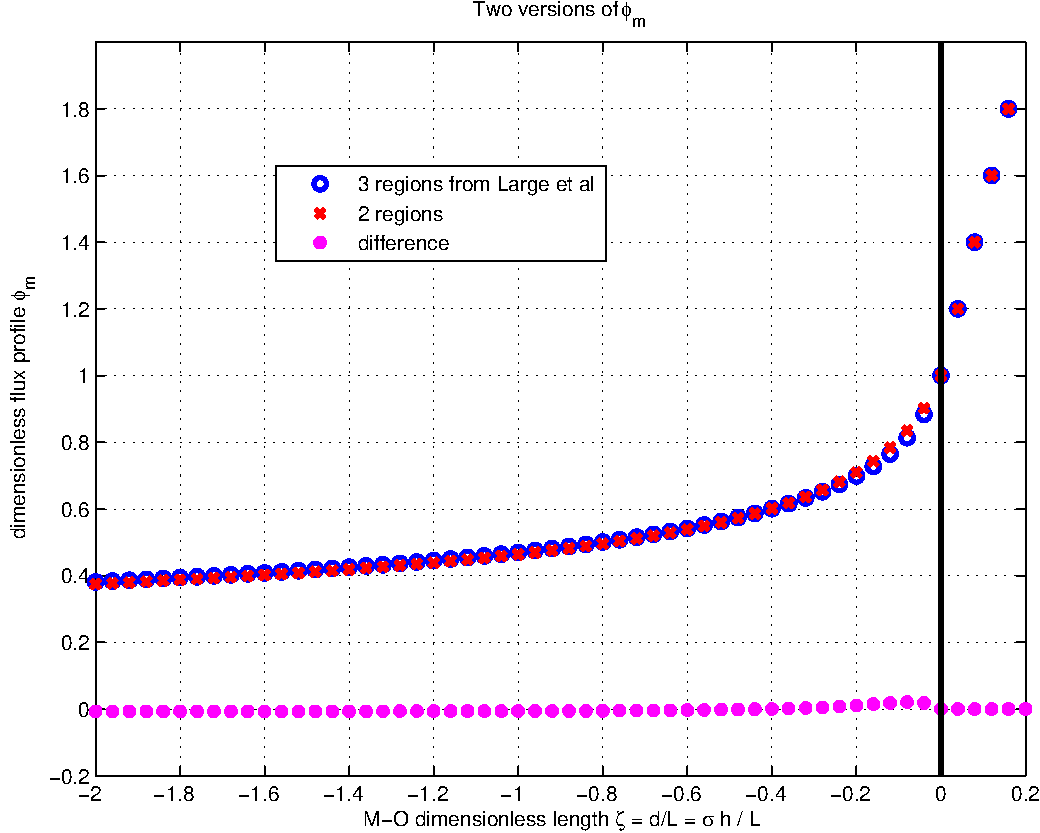
\includegraphics[angle=0,width=8cm,bb=2 0 499 400]{./figs/phi_m_profiles.pdf}
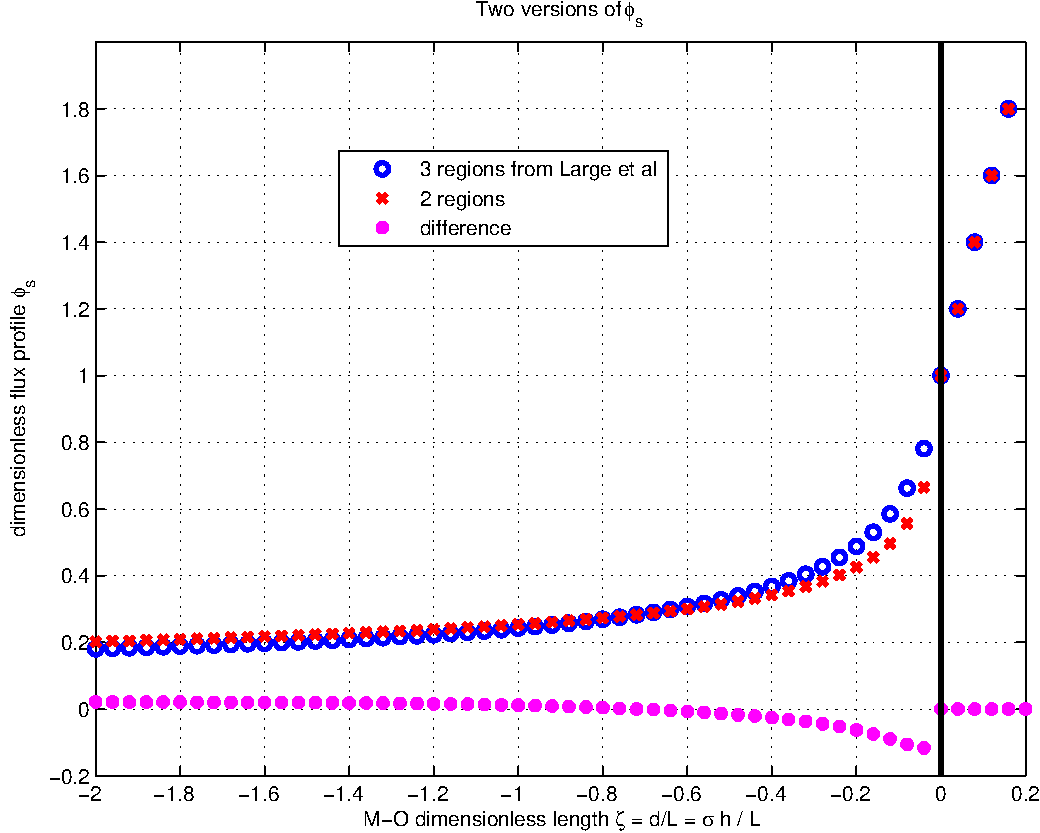
\includegraphics[angle=0,width=8cm,bb=2 0 499 400]{./figs/phi_s_profiles.pdf}
\\
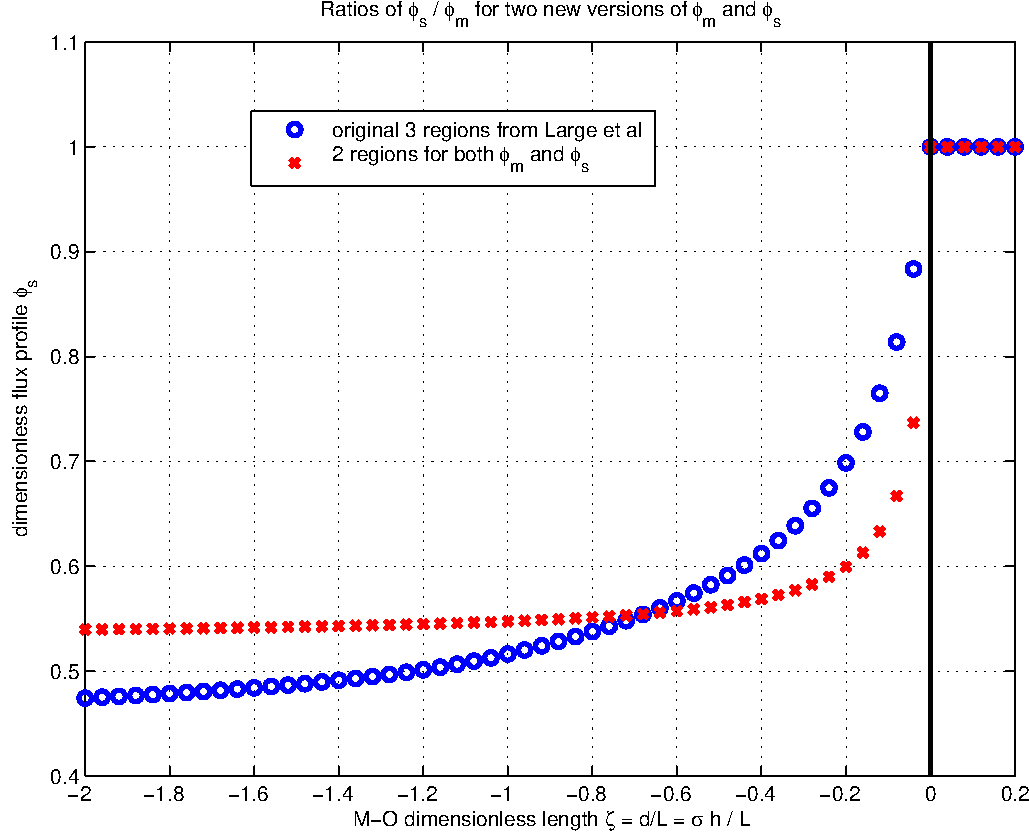
\includegraphics[angle=0,width=8cm,bb=3 0 494 400]{./figs/prandtl_profiles_phim_phis.pdf}
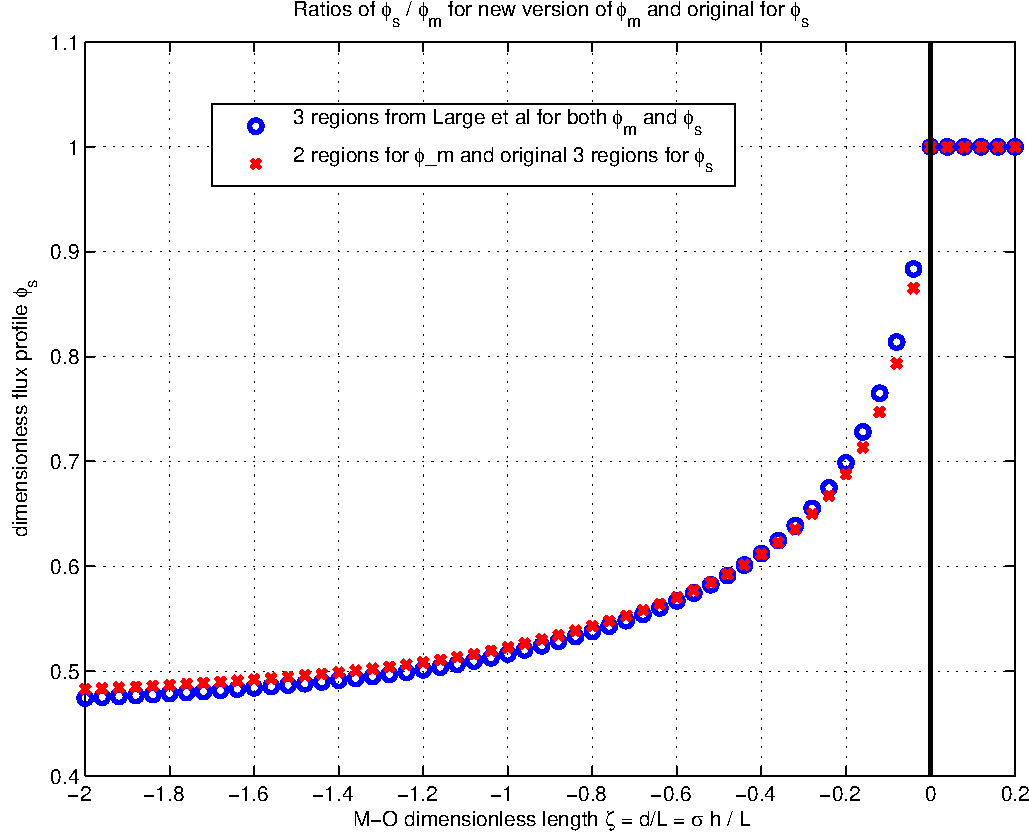
\includegraphics[angle=0,width=8cm,bb=3 0 494 400]{./figs/prandtl_profiles_just_phim_new.pdf}
\caption[Alternative similarity functions]{\sf Shown here are 2-region
  flux profiles given by equations (\ref{eq:phim-alternative}) and
  (\ref{eq:phis-alternative}) as compared to the original 3-region
  profiles rom \cite{LargeKPP}.  We also show the ratio,
  $\phi_{s}/\phi_{m}$, which defines the turbulent Prandtl number or
  the ratio of the vertical momentum viscosity to vertical tracer
  diffusivity.  The top left panel shows the original 3-region
  $\phi_{m}$ as compared to the 2-region form
  (\ref{eq:phim-alternative}).  The agreement is quite close.  The top
  right panel shows the comparison for $\phi_{s}$, with the agreement
  not very good. The lower left panel shows the ratio
  $\phi_{s}/\phi_{m}$ for the original 3-region functions and the new
  2-region functions.  Their ratio amplifies the problems with the new
  $\phi_{s}$ form (\ref{eq:phis-alternative}).  The lower right panel
  shows the ratio of the original 3-region $\phi_{s}$ to the new
  2-region form of $\phi_{m}$.  These results suggest that to remain
  consistent with the original \cite{LargeKPP} results, it is feasible
  to switch to the 2-region form (\ref{eq:phim-alternative}) for
  $\phi_{m}$, but we must maintain the original 3-region form of
  $\phi_{s}$.}
\label{fig:phi-alternative-kpp}
\end{center}
\end{figure}
%%%%%%%%%%%%%%%%%%%%%%%%%%%%%%%%%%%%%%%%%%%%%%%%%%%%%%%%%%%%%%%%%%%%%%%%


\subsection{The shape function $G_{\lambda}(\sigma)$}
\label{subsection:kpp-shape-function}

The vertical shape function $G_{\lambda}(\sigma)$ is given by the cubic
polynomial 
\begin{equation}
 G_{\lambda}(\sigma) = a_{0} + a_{1} \, \sigma + a_{2} \, \sigma^{2} + a_{3} \, \sigma^{3}.
\label{eq:structure-function-gsigma-again}
\end{equation}
As already noted when introducing this cubic expression (equation
(\ref{eq:structure-function-gsigma})), turbulent eddies do not cross
the ocean surface at $\sigma=0$, so the diffusivity should vanish at
$\sigma=0$.  This constraint is satisfied by setting
\begin{equation}
 a_{0} = 0.
\end{equation}
We now discuss further constraints to specify the remaining
coefficients.  

We start by rewriting the expression
(\ref{eq:specifying-structure-function}) that expresses the ratio of
turbulent fluxes within the surface layer to those at the surface
boundary 
\begin{equation}
  a_{1} + a_{2} \, \sigma = \left( \frac{ \overline{w \, \lambda}^{\sigma}}{\overline{w \, \lambda}^{\eta}} \right)
 \qquad  \mbox{surface layer: $0 \le \sigma \le \epsilon$.}
\label{eq:specifying-structure-function-again}
\end{equation}
Satisfying this relation at the ocean surface, $\sigma=0$, requires
\begin{equation}
 a_{1} = 1, 
\end{equation}
 so that 
\begin{equation}
  1 + a_{2} \, \sigma = \left( \frac{ \overline{w \, \lambda}^{\sigma}}{\overline{w \, \lambda}^{\eta}} \right)
 \qquad  \mbox{surface layer: $0 \le \sigma \le \epsilon$.}
\label{eq:specifying-structure-function-againB}
\end{equation}

Now define the ratio
\begin{equation}
  \beta_{\lambda} = \left( \frac{ \overline{w \, \lambda}^{\epsilon}}{\overline{w \, \lambda}^{\eta}} \right),
\end{equation}
which is the ratio of the turbulent flux at the base of the surface
layer, $\sigma = \epsilon$, to the flux at the upper ocean interface,
$z=\eta$.  For atmospheric boundary layers, \cite{Troen_Mahrt1986} set
\begin{equation}
 \beta_{\lambda}  = 2 \, \epsilon \qquad \mbox{atmospheric boundary layers,} 
\end{equation}
with $\epsilon=0.1$.  \cite{Troen_Mahrt1986} further assume both the
shape function and its first derivative vanish at the base of the
boundary layer, $\sigma=1$.  These assumptions lead to the cubic
expression valid for all fluctuating fields $\lambda$
\begin{equation}
 G(\sigma) = \sigma \, (1-\sigma)^{2}   \qquad \mbox{atmospheric boundary layers,}
\end{equation}
with this function exhibited in the left panel of Figure
\ref{fig:kpp-figure2-reproduced}.  

\cite{LargeKPP} also assume the surface layer is 10\% of the boundary
layer, so that 
\begin{equation}
 \epsilon = 0.1 \qquad \mbox{KPP scheme.}
\end{equation}
However, they consider a more general approach for the remaining
approach to deriving the shape function.  The key reason to generalize
the atmospheric approach of \cite{Troen_Mahrt1986} is to admit the
possibility of ocean boundary layer turbulence to be impacted by
interior mixing, with this mixing parameterized by downgradient
vertical diffusion.  Such diffusion generally introduces distinct
diffusivities for tracers (e.g., double diffusion) as well as for
momentum (e.g., non-unit Prandtl number).  For these reasons,
\cite{LargeKPP} insist that both the diffusivity and its vertical
derivative match across the base of the boundary layer at $\sigma=1$.
This matching condition leads to the constraints (18) given by
\cite{LargeKPP}, which in turn leads to shape functions that are
dependent on the field being transported.

Matching both the shape function and its vertical derivative across
the boundary layer base adds complexity to the KPP algorithm.
Furthermore, it is unclear how accurate one can in fact satisfy both
matching conditions on a finite grid with potentially coarse vertical
grid spacing at the boundary layer base.  To simplify the KPP
algorithm, we drop the need to match the vertical derivative of the
diffusivity.  Instead, we assume continuity of the diffusivity with a
vanishing derivative at the boundary layer base, $\sigma=1$.  Setting
$\partial_{\sigma} G(\sigma) = 0$ at $\sigma=1$ leads to the relation
\begin{equation}
 3 \, a_{3} = -(1+ 2 \, a_{2}). 
\label{eq:a3-in-terms-of-a2}
\end{equation}
Matching diffusivities at $\sigma=1$ between the boundary layer and
interior value leads to
\begin{equation}
  a_{2}  = -2 + \left(\frac{3 \, K_{\lambda}(h)}{h \, w_{\lambda}(h)}
  \right),
\label{eq:a2-specified}
\end{equation}
where the diffusivity $K_{\lambda}(h)$ is determined by
parameterizations of interior mixing.  Substituting this expression
for $a_{2}$ into equation (\ref{eq:a3-in-terms-of-a2}) for $a_{3}$
leads to
\begin{equation}
 a_{3} = 1 - \left(\frac{2 \, K_{\lambda}(h)}{h \, w_{\lambda}(h)} \right).
\end{equation}
Allowing for the interior mixing to influence the KPP boundary layer
scheme suggests that the KPP calculation should be called {\it after}
the various methods used to compute interior diffusivities.  



\subsection{The non-local transport $\gamma_{\lambda}$}
\label{subsection:kpp-non-local-transport}

We now consider the parameterization for the non-local transport (see
Section \ref{subsection:kpp-nonlocal-transport-outline}) as suggested
by \cite{LargeKPP}.  Again, the KPP parameterization takes the form
(equation (\ref{eq:kpp-parameterization}))
\begin{equation}
  \overline{w \, \lambda} = -K_{\lambda} \left( \frac{\partial \Lambda}{\partial z} - \gamma_{\lambda} \right),
\label{eq:kpp-parameterization-yet-again}
\end{equation}
so that that non-local portion of the turbulent flux is parameterized
according to
\begin{equation}
 \overline{w \, \lambda}^{\mbox{\tiny non-local}} = K_{\lambda}  \, \gamma_{\lambda},  
\end{equation}
where $K_{\lambda}$ takes the form in equation
(\ref{eq:kpp-diffusivity-again}): 
\begin{equation}
 K_{\lambda}(\sigma) = h \, w_{\lambda}(\sigma) \, G_{\lambda}(\sigma).
\label{eq:kpp-diffusivity-yet-again}
\end{equation}
For completeness, we repeat elements of the outline presented in
Section \ref{subsection:kpp-nonlocal-transport-outline}.


\subsubsection{General features of $\gamma_{\lambda}$ with the KPP parameterization}

\begin{itemize}

\item \cite{Smyth_etal2002} consider a non-local term for momentum.
  Until their ideas have been fully tested in climate models, we
  follow recommendations from \citep{LargeKPP}, who set the non-local
  momentum transport to zero:
\begin{equation}
 \gamma_{\lambda} \; \; = \; \; 
\left\{
 \begin{array}{ll}
  0 \; \;  &\mbox{if $\lambda = (u,v,w)$ a velocity component}
 \\
  \ne 0 \; \; &\mbox{nonzero if $\lambda = \theta,s$ or another tracer.}
  \end{array}
 \right.
\end{equation}

  \item The non-local transport is non-zero only within the OBL:  
\begin{equation}
 \gamma_{\lambda} \; \; = \; \; 
  \left\{ 
  \begin{array}{ll}
   0 \; \; &\mbox{if $\sigma > 1$}
   \\ 
   \ne 0  \; \; &\mbox{if $0 \le \sigma \le 1$.}
  \end{array}
 \right.
\end{equation}

  \item The non-local transport is non-zero only in the presence of
    destabilizing negative surface ocean buoyancy flux:
\begin{equation}
 \gamma_{\lambda} \; \; = \; \; 
  \left\{ 
  \begin{array}{ll}
   0 \; \; &\mbox{for $B_{f} > 0$}
   \\ 
   \ne 0 \; \; &\mbox{for $B_{f} < 0$.}
  \end{array}
 \right.
\end{equation}


\item The non-local transport for temperature and arbitrary scalars is
  given by the following form for destabilizing negative surface ocean
  buoyancy fluxes:
\begin{align}
 \gamma_{\theta} &= 
   C_{s} \, \left( \frac{ \overline{w \, \theta}^{\eta} - Q_{R}/(\rho_{0} \, C_{p})  }{h \,  w_{\theta}(\sigma)}  
            \right) 
\label{eq:non-local-temp-kpp}
\\
 \gamma_{s} &= 
   C_{s} \, \left( \frac{ \overline{w \, s}^{\eta} }{h \,  w_{s}(\sigma)}  
            \right), 
\label{eq:non-local-scalar-kpp}
\end{align}
 where 
\begin{equation}
 C_{s} = C_{*} \, \kappa \, (c_{s} \, \kappa \, \epsilon)^{1/3},  
\end{equation}
with 
\begin{equation}
 C_{*} = 10,
\end{equation}
and $Q_{R}$ is the heat flux from penetrative radiation given by
equation (\ref{eq:penetrative-heating-kpp}).

Combining the parameterizations (\ref{eq:non-local-temp-kpp}) and
(\ref{eq:non-local-scalar-kpp}) for the non-local term
$\gamma_{\lambda}$, with that for the vertical diffusivity
$K_{\lambda}$ in equation (\ref{eq:kpp-diffusivity-yet-again}) renders
the non-local flux parameterization in the form
\begin{align}
\overline{w \, \theta}^{\mbox{\tiny non-local}} &= K_{\theta}  \, \gamma_{\theta}
  = 
 G_{\lambda}(\sigma) \, C_{s} \, \left( \overline{w \, \theta}^{\eta} - Q_{R}/(\rho_{0} \, C_{p}) \right)
\label{eq:non-local-flux-kpp-param-temp}
\\
\overline{w \, s}^{\mbox{\tiny non-local}} &= K_{s}  \, \gamma_{s}
  = 
 G_{s}(\sigma) \, C_{s}\,\left( \overline{w \, s}^{\eta} \right).
\label{eq:non-local-flux-kpp-param-scalar}
\end{align}
Notice how explicit dependence on both the turbulent velocity scale,
$w_{\lambda}$, and boundary layer depth, $h$, drop out from the
parameterization of the non-local flux.

\end{itemize}


\subsubsection{Potential problems with the parameterized non-local transport}

Experience has shown that there are cases when the parameteried
non-local flux, (\ref{eq:non-local-flux-kpp-param-temp}) of
(\ref{eq:non-local-flux-kpp-param-scalar}), can produce values larger
than the surface flux.  That is, one may realize cases when 
\begin{equation}
   G_{\lambda}(\sigma) \, C_{s} > 1 \qquad \mbox{non-local flux greater than surface flux.}
\end{equation}
This situation arises particularly near the boundary layer base,
$\sigma=1$, when the interior diffusivity is large.  The matching
conditions employed by \cite{LargeKPP} (Section
\ref{subsection:kpp-shape-function}) then lead to a very large value
for the shape function $G(\sigma)$.  In this case, one may be exposed
to the production of extrema in the tracer field.  In the presence of
sea-ice, problems may arise particularly in fresh water regions such
as the Baltic Sea where the thermal expansion coefficient is negative,
$\alpha < 0$ (Martin Schmidt, personal communication).

The following modifications to the original \cite{LargeKPP} scheme
have been found useful to reduce the potential for the non-local term
to be problematic. 
\begin{itemize}

\item {\sc interior gravitational instabilities}: When the vertical
 stratification is unstable ($N^{2} < 0$), vertical diffusivity is
  enhanced to remove the gravitational instability. Notably, it is
  {\it not} appropriate to enhance the diffusivity within the KPP
  boundary layer, beyond that already computed via the KPP scheme,
  even when $N^{2} < 0$.  On those occasions when the instabilities
  appear beneath the boundary layer, diffusivities are enhanced.  If
  one insisted that such diffusivities should match those in the
  boundary layer, then the shape function $G(\sigma)$ would indeed
  become quite large in magnitude.  Hence, NCAR recommends that one
  pull the ``convective adjustment'' portion of the mixing scheme
  outside of the KPP portion of the algorithm.  That is, the interior
  convective instability diffusivities are {\it not} matched to the
  KPP boundary layer diffusivities.  

\item {\sc simpler matching}: As noted in Section
  \ref{subsection:kpp-shape-function}, we propose to simplify the
  matching at the boundary layer base, so that only the diffusivities
  match across the boundary layer base, rather than also insisting on
  the derivative of the diffusivities as proposed by \cite{LargeKPP}.
  The simplified matching condition leads to less problems computing
  discrete vertical derivatives of the diffusivities, and in turn
  produces more well regularized diffusivities and shape functions.

\end{itemize}


\subsection{Bulk Richardson number and the OBL thickness}
\label{subsection:kpp-obl-thickness}

\cite{LargeKPP} define the KPP boundary layer depth to be an
interpolation to the depth at which the bulk Richardson number,
$\mbox{Ri}_{b}$, equals to a critical Richardson number,
$\mbox{Ri}_{c}$.  Smaller values for $\mbox{Ri}_{b}$, including
negative values, signal that we are still in the boundary layer,
whereas larger values are beneath.  The critical value $\mbox{Ri}_{c}$
sets a threshold for upper ocean mixing, with such enabling behaviour
that is sensitive to its precise value.

The bulk Richardson number is a non-local version of the gradient
Richardson number defined in Section
\ref{section:gradient-richardson-number-elements}.  It aims to measure
the ability of an upper ocean eddy, with buoyancy set by values of
temperature and salinity in the surface layer (Figure
\ref{fig:boundary-layer-schematic-kpp}), to move downward in the water
column, overcoming the resistence from stratification and aided by
both resolved and unresolved vertical shear.  Presumably at some
point, such boundary layer eddies will be suppressed by the reduced
shear and increased buoyancy stratification present below the boundary
layer.

Using the notation from \cite{LargeKPP}, we may write the bulk
Richardson number at a distance $d$ from the ocean surface in the form
\begin{equation}
  \mbox{Ri}_{b}(d) = \frac{d \, [B_{r} - B(d) ]}{ |{\bf U}_{r} - {\bf U}(d)|^{2} + U_{t}^{2}}. 
\label{eq:bulk-ri-large-kpp-large-etal-form}
\end{equation}
This calculation makes use of the surface layer averaged buoyancy,
$B_{r}$, and surface layer averaged horizontal velocity, ${\bf
  U}_{r}$, where the surface layer is defined by $0 \le \sigma \le
\epsilon$ (Figure \ref{fig:boundary-layer-schematic-kpp}). The term
$U_{t}^{2}$ is associated with parameterized unresolved vertical
shears that may act to further reduce the bulk Richardson number.

Using notation introduced in the local gravitational stability
calculation from Section \ref{section:buoyancy-frequency-elements}, we
write the bulk Richardson number in the form
\begin{equation}
  \mbox{Ri}_{b}(d) = \left( \frac{d \, g}{\rho_{o}} \right) 
   \left( 
   \frac{\rho[\Theta(d), S(d), p(d)]   - \rho[\Theta_{r}, S_{r}, p(d)]}{ |{\bf U}_{r} - {\bf U}(d)|^{2} + U_{t}^{2}}
  \right). 
\label{eq:bulk-ri-large-kpp}
\end{equation}
The density $\rho[\Theta(d), S(d), p(d)]$ is the {\it in situ} value
at a distance $d$ from the surface.  The density $\rho[\Theta_{r},
S_{r}, p(d)]$ is based on an adiabatic and isohaline displacement from
the surface layer to the depth $d$.  Now consider three cases to
expose the physics of the bulk Richardson number.
\begin{itemize}

\item {\sc Surface eddy has negative relative buoyancy}: If the
  density $\rho[\Theta_{r}, S_{r}, p(d)]$ is greater than the {\it in
    situ} density, $\rho[\Theta(d), S(d), p(d)]$, then a surface layer
  parcel can move downwards and the boundary layer based has yet to be
  reached.  That is, the surface layer parcel has negative buoyancy
  relative to the ambient fluid.  This situation leads to a negative
  bulk Richardson number, in which case the criteria $\mbox{Ri}_{b}(d)
  > \mbox{Ri}_{c}$ has not yet been reached.

\item {\sc Surface eddy has positive relative buoyancy and ambient
    fluid has strong shears}: If the density $\rho[\Theta_{r}, S_{r},
  p(d)]$ is less than the {\it in situ} density, a surface layer eddy
  has positive buoyancy relative to the ambient fluid.  However, if
  the vertical shear is large, then the bulk Richardson number can
  still be less than the critical value, in which case mechanically
  induced mixing is still large and the boundary layer base has yet to
  be reached.

\item {\sc Surface eddy has positive relative buoyancy and ambient
    fluid has weak shears}: Finally, if a surface eddy has positive
  relative buoyancy and the ambient fluid has weak shears, then at
  some point the bulk Richardson number will become larger than the
  critical value.  Interpolating to where that cross-over occurs
  determines the boundary layer thickness $h$.  

\end{itemize}


\subsubsection{Non-local gravitational stability}

Section \ref{section:buoyancy-frequency-elements} presents a general
discussion of local gravitational stability.  Much of that material is
useful for the purpose of determining gravitational stability for
parcels that are a finite distance from one another.  However, there
is one aspect of the discussion in Section
\ref{section:buoyancy-frequency-elements} that differs from the
present considerations.  Namely, we are here always considering
downward displacements of parcels from the surface layer.  The reason
is that we are concerned with parcels starting from the surface layer
moving downwards in an adiabatic and isohaline manner, with the
difficulty of such motion determined by the ambient stratification and
shear.  Figure \ref{fig:cvmix_stability_nonlocal} illustrates this
situation.  We are not interested in the complement movement of a deep
parcel towards the surface.


%%%%%%%%%%%%%%%%%%%% %%%%%%%%%%%%%%%%%%%%%%%%%
\begin{figure}[h!t]
\begin{center}
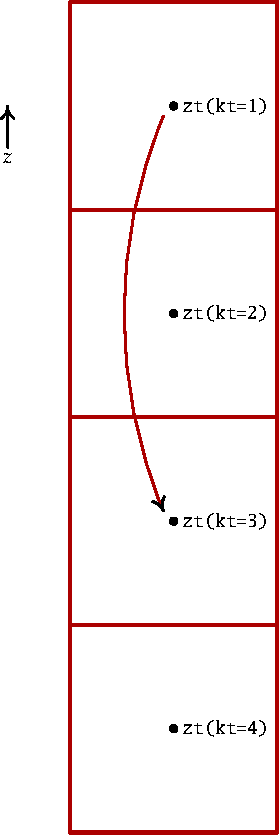
\includegraphics[angle=0,width=3cm,bb=0 0 134 401]{./mfpic_figs/cvmix_stability_nonlocal.pdf}
\caption[Determining non-local gravitational stability]{\sf Schematic
  of the adiabatic and isohaline parcel displacement that is used to
  determine non-local gravitational stability for computing the bulk
  Richardson number according to equation
  (\ref{eq:bulk-ri-large-kpp}).  The reference temperature and
  salinity of this displaced parcel is set according to values
  determined in the surface layer, here approximated by the value at
  the top model grid cell with vertical position {\tt zt(kt=1)}.  The
  density of this parcel is then computed using the surface layer
  temperature and salinity and the local {\it in situ} pressure.  This
  displaced parcel's density is then compared to the ambient {\it in
    situ} density using the local temperature, salinity, and pressure.
  We illustrate that process by displacing the parcel to {\tt
    zt(kt=3)}.  If the resulting bulk Richardson number is larger than
  the critical value, the base of the KPP boundary layer is at or
  shallower than {\tt zt(kt=3)}, with interpolation used to determine
  the KPP boundary layer thickness $h$.  If the bulk Richarson number
  is less than the critical value, the boundary layer bottom has yet
  to be reached, so the downward search continues.}
\label{fig:cvmix_stability_nonlocal}
\end{center}
\end{figure}
%%%%%%%%%%%%%%%%%%%%%%%%%%%%%%%%%%%%%%%%%%%%%%%%%%%%%%%%%%%%%%%%%%%%%%%%

The expression (\ref{eq:bulk-ri-large-kpp}) presents a direct means
for computing the non-local gravitational stability via the
computation of the density difference, written here using discrete
notation from Figure  \ref{fig:cvmix_stability_nonlocal}
\begin{equation}
 \delta\rho[{\tt kt},r]  = \rho[\Theta({\tt kt}), S({\tt kt}), p({\tt kt} ]  -\rho[\Theta_{r}, S_{r}, p({\tt kt})],
\label{eq:delta-density-for-nonlocal-stability}
\end{equation}
where the surface layer values $\Theta_{r}, S_{r}$ are typically
approximated by the values as {\tt kt =1}.  This approximation breaks
down for stable boundary layers with vertical grid spacing finer than
roughly 2~m, in which case an averaging is required.

There is an alternative method to approximate $\delta\rho[{\tt kt},r]$
based on linear truncations of Taylor series expansions.  The
alternative leads to a sum of squared buoyancy frequencies, analogous
to the expression
(\ref{eq:inifinitesimal-delta-rho-elements-downward}).  There are some
advantages offered by the alternative approach, namely there are fewer
calculations of the equation of state, assuming we already have the
expansion coefficients $\alpha$ and $\beta$.  However, the deeper the
boundary layer, and the more nonlinear the equation of state, the less
accurate the approximation becomes.  We therefore recommend the more
exact calculation based on the density differences in equation
(\ref{eq:delta-density-for-nonlocal-stability}).

For completeness, we develop the alternative approach.  For this
purpose, consider a displacement from level {\tt kt = 1} to {\tt kt
  >1}, in which we need to compute $\rho[\Theta({\tt kt=1}),S({\tt
  kt=1}),p({\tt kt>1})]$.  Truncating a Taylor series at leading order
yields
\begin{equation}
 \rho[\Theta(1),S(1),p({\tt kt>1})]
 \approx 
 \rho[\Theta(1),S(1),p(1)] 
 - \sum\limits_{{\tt n  = 1}}^{{\tt kt}}
   {\tt dzw(n+1)} \,  \left( \frac{\partial \rho}{\partial p} \, \frac{\partial p}{\partial z}
   \right)_{ {\tt zt(n)} }.
\end{equation}
A similar expression for the {\it in situ} density $\rho[\Theta({\tt
  kt}), S({\tt kt}), p({\tt kt} ]$
\begin{equation}
 \rho[\Theta({\tt kt}),S({\tt kt}),p({\tt kt})]
 \approx 
 \rho[\Theta(1),S(1),p(1)] 
 - \sum\limits_{{\tt n  = 1}}^{{\tt kt}}
   {\tt dzw(n+1)} \,  \left( 
   \frac{\partial \rho}{\partial p} \, \frac{\partial p}{\partial z}
   + 
  \frac{\partial \rho}{\partial \Theta} \, \frac{\partial \Theta}{\partial z}
  +
  \frac{\partial \rho}{\partial S} \, \frac{\partial S}{\partial z}
   \right)_{ {\tt zt(n)} }.
\end{equation}
These results lead to the approximation 
\begin{equation}
\begin{split}
 \delta\rho[{\tt kt},r]  &= \rho[\Theta({\tt kt}), S({\tt kt}), p({\tt kt} ]  -\rho[\Theta_{r}, S_{r}, p({\tt kt})]
 \\
 &\approx 
 -\sum\limits_{{\tt n  = 1}}^{{\tt kt}}
   {\tt dzw(n+1)} \,  \left( 
 \frac{\partial \rho}{\partial \Theta} \, \frac{\partial \Theta}{\partial z}
  +
  \frac{\partial \rho}{\partial S} \, \frac{\partial S}{\partial z}
   \right)_{ {\tt zt(n)} }
\\
 &=
 \sum\limits_{{\tt n  = 1}}^{{\tt kt}}
   {\tt dzw(n+1)} \,  \left( 
 \rho \, \alpha \, \frac{\partial \Theta}{\partial z}
  -
  \rho \, \beta \, \frac{\partial S}{\partial z}
   \right)_{ {\tt zt(n)} }
\\
 &= 
 \frac{1}{g} 
  \sum\limits_{{\tt n  = 1}}^{{\tt kt}}
   {\tt dzw(n+1)} \,  \left( \rho \, N^{2} \right)_{ {\tt zt(n)} }.
\end{split}
\label{eq:summed-n2-for-nonlocal-stability}
\end{equation}
Again, this result is analogous to the approximate forms given in
Section \ref{subsection:buoyancy-frequency-and-stability} for the
local calculation of gravitational stability.  For that calculation,
it is sensible to drop the higher order terms in the Taylor
series. However, for the non-local calculation considered here, one
may in fact be compromising the determination of gravitational
stability, particularly in regions of deep mixing in the high
latitudes. We may also be compromising the ability of the KPP scheme
to include thermobaric convection.  We are thus reticent to recommend
this approach, and instead prefer the original approach given by
equation (\ref{eq:bulk-ri-large-kpp}).


\subsubsection{Unresolved shear $U_{t}$}

The shear, $U_{t}/d$, in the bulk Richardson number
(\ref{eq:bulk-ri-large-kpp}) acknowledges the potential presence of
unresolved shears that can impact on the boundary layer depth.
\cite{LargeKPP} present an argument on page 372 that focuses on an
unresolved shear that reduces to a desired form for the case of pure
convection
\begin{equation}
 U_{t}^{2}(d) = \frac{C_{v} \, (-\beta_{T})^{1/2}}{\mbox{Ri}_{c} \, \kappa^{2}}
  (c_{s} \, \epsilon)^{-1/2} \, d \; N \; w_{s}.
\label{eq:unresolved-shear-kpp}
\end{equation}
 The constant $C_{v}$ sets the buoyancy frequency at the entrainment
 depth, and its value is expected to be 
\begin{equation}
 1 < C_{v} < 2.  
\end{equation}
The constant $c_{s}$ is part of the similarity functions discussed in
Section \ref{subsection:m-o-similarity-functions}.  The constant
$\beta_{T}$ is discussed in the caption to Figure
\ref{fig:kpp-figure1-reproduced}, and is represents the ratio of the
buoyancy flux at the entrainment depth, $h_{e}$, to the buoyancy flux
at the surface,
\begin{equation}
 \overline{w \, b}^{d=h_{e}} = -\beta_{T}   \; \overline{w \, b}^{d=0},
\end{equation}
 with 
\begin{equation}
 \beta_{T} \approx 0.2
\end{equation}
an empirical result.  The critical Richardson number, $\mbox{Ri}_{c}$, is
used to determine when the boundary layer base is reached, in which
case stratification and/or reduced shear lead to a bulk Richardson
number larger than the critical value.  \cite{LargeKPP} choose the
value
\begin{equation}
 \mbox{Ri}_{c} = 0.3.  
\end{equation}
The dimensionless number $\epsilon$ determines the thickness of the
surface layer as in Figure \ref{fig:boundary-layer-schematic-kpp},
with 
\begin{equation}
 \epsilon = 0.1 
\end{equation}
 chosen by \cite{LargeKPP}. 

It is notable that there are no surface gravity wave parameters in the
specification of the unresolved shear.  We have more to say on this
topic in Section \ref{section:surface-waves-and-kpp}. 


\subsubsection{Restrictions on $h$ under stable buoyancy forcing}

\cite{LargeKPP} suggest on page 372 that for stable buoyancy forcing,
$B_{f} > 0$, the boundary layer thickness, $h$, should be no larger
than either the Monin-Obukhov length scale, $L$, or the Ekman
length scale, 
\begin{equation}
 h_{E} = 0.7 \; u_{*} /f,
\label{eq:ekman-thickness}
\end{equation} 
with $f$ the Coriolis parameter.  The following reasons are noted to
motivate these two restrictions.
\begin{itemize}
\item {\sc Monin-Obukhov}: At depths deeper than $L$, buoyancy
  stratification suppresses the mechanically forced turbulence, thus
  cutting off the boundary layer.

  \item {\sc Ekman}: The Ekman depth is the extent of the boundary
    layer in neutral stratification ($N^{2} = 0$).  With stable
    buoyancy forcing, $B_{f} > 0$, we then expect the boundary layer
    depth to be less than the Ekman depth.  Note that \cite{LargeKPP}
    do not mention the origin of the $0.7$ factor in equation
    (\ref{eq:ekman-thickness}).

\end{itemize}

As noted in \cite{LargeKPP} and \cite{Large_Gent1999}, the restriction
based on the Monin-Obukhov has been dropped in the NCAR implementation
of KPP, as it does not lead to favorable effects.  Dropping this
constraint is also supported by the results from
\cite{Shchepetkin2005} and \cite{Lemarie_etal2012a}.  Likewise, the
constraint based on the Ekman depth is not used at NCAR, as little
sensitivity was seen with its use.  Hence, there are no restrictions
for the maximum boundary layer depth under stable forcing imposed by
the NCAR implementation of KPP.  Such is the standard approach used in
the CVMix implementation.

The key problem with the Monin-Obukhov length scale, $L$, relates to
the question of how to include penetrative shortwave heating in the
calculation of the buoyancy forcing, $B_{f}$ (Section
\ref{subsection:buoyancy-forcing-obl}).  Depending on the depth over
which the penetrative heating is included (equation
(\ref{eq:penetrative-buoyancy-kpp})), one can produce a positive
Monin-Obukhov length (if including sufficient shortwave heating) or
negative (if including less heating). Since there is no fundamental
reason to choose a particular amount of the shortwave when considering
the total buoyancy forcing, there is no compelling reason to enforce
the $L$ constraint on boundary layer thickness.


\subsubsection{Noise in the boundary layer thickness}

Experience in MOM, POP, and ROMS indicate that the KPP boundary layer
thickness, $h$, can become quite noisy.  Noise in the boundary layer
thickness can translate into noise in the tracer fields within the
boundary layer.  Hence, it is common practice to apply a horizontal
smoothing operator, such as a Laplacian, to $h$ prior to its use in
computing the diffusivity or non-local transport.

The horizontal smoothing of $h$ poses an algorithmic problem for
CVMix, since CVMix modules ideally know nothing about the horizontal
grid.  There are two possible options that may be considered.
\begin{itemize}

\item {\sc intermediate $h$ sent back to calling model}: One option is
  to compute $h$ in CVMix; send it immediately back to the
  calling model for smoothing; then have the smoothed $h$ used for
  further KPP computations such as the diffusivity and non-local
  term.  

\item {\sc use previous $h$}: We compute the new value of $h$ within a
  particular call to the CMVix-KPP module, and we send this unsmoothed
  $h$ back to the calling model at the end of the CVMix-KPP module.
  But for computing the KPP diffusivities and non-local term within
  CVMix, we use the previous time step value $h$, with this earlier $h$
  having been smoothed by the calling model.  This approach requires
  storing $h$ in restart files, but that is easily handled by the
  calling model.  

\end{itemize}




\section{KPP with surface waves}
\label{section:surface-waves-and-kpp}

\cite{Craig_Banner_1994} considered surface waves in a modification of
the \cite{MellorYamada1982} 2.5 order turbulence scheme.
\cite{Axell_2002} considered also Langmuir turbulence in the
$k-\epsilon$ closure scheme.  We consider here some issues related to
introducing both waves and Langmuir turbulence in the KPP scheme.

The KPP formulation presented by \cite{LargeKPP} ignores surface waves
and the associated breaking waves and Langmuir turbulence.  The basis
for KPP must be revisited in regions of waves, since waves modify the
Monin-Obukhov similarity scalings (see \cite{Terray_etal1996} for the
case of breaking waves, and Section 2.2 of
\cite{SullivanMcWilliams2010} for wave-driven winds).  In the presence
of waves, the ocean surface contains both breaking waves to enhance
upper ocean mixing and dissipation; swell, which can modify the the
atmospheric planetary boundary layer by providing momentum to lower
atmospheric winds; and the coupling of Stokes drift to currents to
produce Langmuir cells and associated turbulence
\citep{McWilliams_etal1997}.  These processes act in addition to and
in interaction with the shear induced eddies and buoyant plumes
traditionally considered as part of the KPP scheme.  The modifications
to KPP with waves represents a research project, with work from
\cite{Belcher_etal2012} a step towards this goal, in which they
consider the regimes where winds are more or less important than
Langmuir turbulence.

In this section, we identify some incremental steps that may be
considered for modifying aspects of KPP to incorporate features of
surface waves.  Even with these more humble aspirations, there are
many questions.


\subsection{Modified budgets with Stokes velocity}
\label{subsection:stokes-into-pe-kpp}

Large eddy simulations that incorporate surface waves, such as those
from \cite{McWilliamsSullivanMoeng1997}, \cite{McWilliamsSullivan2001}
and \cite{SullivanMcWilliams07}, include a contribution in the
momentum equation from the Stokes velocity on the Coriolis force as
well as a vortex force.  Additionally, the tracer equation includes
advection from the Stokes velocity.  Finally, the subgrid scale
turbulent kinetic energy equation also includes advection by the
Stokes velocity, as well as vertical shear of the Stokes velocity
coupled to the subgrid scale stresses, thus acting as a source for
turbulent kinetic energy. Mathematically, these terms take the form
(see equations (4a), (4b) and (4c) from \cite{SullivanMcWilliams2010})
\begin{align}
\frac{\partial {\bf v}}{\partial t} &= \ldots -f \, \hat{\bf z} \, \wedge \, {\bf v}^{\mbox{\tiny stokes}}  
 + {\bf v}^{\mbox{\tiny stokes}}  \, \wedge \, \bfomega
\\
\frac{\partial C}{\partial t} &= \ldots -{\bf v}^{\mbox{\tiny stokes}} \cdot \nabla C
\\
\frac{\partial E}{\partial t} &= \ldots -{\bf v}^{\mbox{\tiny stokes}} \cdot \nabla E
 - \tau_{i3} \frac{\partial v^{\mbox{\tiny stokes}}_{i}}{\partial x_{3}}
\end{align}
where ${\bf v}$ is the velocity field $(u,v,w)$ resolved by the LES,
$\bfomega = \nabla \, \wedge \, {\bf v}$ is the vorticity, ${\bf
  v}^{\mbox{\tiny stokes}}$ is the Stokes velocity due to wave
motions, $C$ is an arbitrary tracer concentration, $E$ is the
turbulent kinetic energy, and $\tau_{ij}$ is the deviatoric
subgrid-scale stress tensor. The dots denote standard terms such as
pressure gradients, friction, etc.

The question arises as to whether a hydrostatic primitive equation
should also modify the prognostic equations for momentum and tracer in
a manner emulating that done for the LES.  We offer the following
reasons to {\it not} do so.
\begin{itemize}

\item In present applications with hydrostatic primitive equation
  ocean models, a wave model provides information about the Stokes
  velocity, or an estimate of this velocity is made based on wind
  stress \citep{Li_Garrett1993}.  However, there is no feedback to the
  waves from the circulation.  Indeed, there is no such feedback
  considered in the LES studies from
  \cite{McWilliamsSullivanMoeng1997}, \cite{McWilliamsSullivan2001}
  and \cite{SullivanMcWilliams07}.  For the primitive equation models
  used for climate research, it would be problematic to have a
  quiescent Eulerian mean flow impacted by a wave to thus initiate
  inertial circulations.  In fact, it is the Stokes circulation itself
  that should be impacted.  

\item The Stokes circulation velocity, ${\bf v}^{\mbox{\tiny stokes}}$,
  is generally considered to have only horizontal components
\begin{equation}
  {\bf v}^{\mbox{\tiny stokes}}  =(u^{\mbox{\tiny stokes}}, v^{\mbox{\tiny stokes}},0)
\end{equation}
These components are horizontally divergent. Hence, their presence in
the flux-form tracer equation appears both as an advection plus a
source term.

\item As discussed by \cite{Rascle_etal2004}, ensemble averaging of
  these equations eliminates the added vortex force term.   

\item There are cases where the large-scale Eulerian mean flow in an
  LES will compensate for the Stokes flow, leading to a vanishing
  Lagrangian mean velocity.  This balance cannot be represented in a
  primitive equation ocean model, so the selective introduction of
  only a piece of the full dynamics can lead to spurious effects.

\end{itemize}
In conclusion, introduction of the Stokes velocity into the tracer and
momentum equations of a hydrostatic primitive equation ocean model is
{\it not} recommended.


\subsection{Modifications from Stokes velocity and Langmuir
  turbulence}
\label{subsection:stokes-langmuir-kpp}

\begin{itemize}

\item It is conjectured that the most important change to KPP may
  arise from enhanced shear due to Stokes velocity when computing bulk
  Richardson number (Section \ref{subsection:kpp-obl-thickness}).  We
  must be careful to note that in some cases, a piece of the Eulerian
  and Stokes velocities in fact cancel, leaving only a residual
  velocity whose vertical shear impacts the bulk Richardson number.
  However, this result needs some care to distinguish the potential
  for this effect to occur on the larger scaled represented in a
  primitive equation model.  Note that for some reason,
  \cite{Smyth_etal2002} do not consider this effect in their
  modifications to KPP from waves and Langmuir turbulence.  Perhaps
  they assume there is a piece of the unresolved Eulerian velocity
  that exactly cancels the Stokes velocity, thus leaving no new
  unresolved term in the bulk Richardson number calculation.

\item There are additional changes to the turbulent velocity scale,
  $w_{\lambda}$, that may arise from Langmuir turbulence.  Questions
  arise regarding the precise calculation of the Langmuir number, the
  scaling added to the turbulence velocity scale, and the depth
  dependence of the Langmuir number.   



\end{itemize}



%\chapter{\scshape Vertical convective mixing}
\label{chapter:cvmix_convection}

\minitoc
\vspace{.5cm}

The purpose of this chapter is to present the vertical convective
mixing scheme available in CVMix.  The following CVMix Fortran module
is directly connected to the material in this chapter:
\begin{align*} 
 &  {\tt cvmix\_convection.F90}.
\end{align*}


\section{Introduction to convective mixing}
\label{section:intro}

The hydrostatic approximation necessitates the use of a
parameterization of vertical overturning processes.  The original
parameterization used by Bryan in the 1960's was motivated largely
from ideas then used for modeling convection in stars
(\cite{Bryan1969}).  Work by Marshall and collaborators
(\cite{KlingerConvection}, \cite{MITgcm}) have largely supported the
basic ideas of vertical adjustment for purposes of large-scale ocean
circulation.

The \cite{CoxModel} implementation of convective adjustment (the
``NCON" scheme) may leave columns unstable after completing the code's
adjustment loop.  Various full convective schemes have come on-line,
with that from \cite{Rahmstorf1993} implemented in MOM.  An
alternative to the traditional form of convective adjustment is to
increase the vertical mixing coefficient to some large value (say $\ge
10 \mbox{m}^{2} \, \mbox{s}^{-1}$) in order to quickly diffuse
vertically unstable water columns.  Indeed, it is this form
recommended from the study of \cite{KlingerConvection}, and it is the
approach commonly used in boundary layer schemes such as \cite{PPvmix}
and \cite{LargeKPP}.  It is this vertical convective mixing approach
that is supported in CVMix.  


\section{Time-implicit vertical mixing}
\label{section:time-implicit-vmix}

An explicit treatment, especially with fine vertical grid resolution,
places an unreasonable limitation on the size of the time step
associated with vertical mixing processes.  The use of fine vertical
resolution with sophisticated mixed layer and/or neutral physics
schemes has prompted the near universal time-implicit treatment of
vertical mixing in ocean climate models.


%\chapter{\scshape Diffusivity based on a chosen dissipation}
\label{chapter:cvmix_dissipate}

\minitoc
\vspace{.5cm}

The purpose of this chapter is to summarize a method that is not
available in CVMix, yet which may be of interest to modellers using
CVMix schemes.  This method specifies vertical tracer diffusivities
based on setting a floor to the power dissipation.  This approach was
found to be useful in the ESM2G earth system model documented by 
\cite{Dunne_etal_part1_2012}.


\section{Power dissipation from vertical diffusion}
\label{section:vert_dissipation_formulation}

Vertical tracer diffusion is associated with a dissipation of power.
Assuming temperature and salinity have the same vertical diffusivities
leads to the expression for power dissipation
($\mbox{W}~\mbox{m}^{-3}$)
\begin{equation}
\begin{split}
 \epsilon &= \rho \,  \kappa \, N^{2}
 \\
&= -\kappa \, g \, \left( \frac{\partial \rho}{\partial \theta} \, \frac{\partial \theta}{\partial z} 
                                      +\frac{\partial \rho}{\partial S}         \, \frac{\partial S}{\partial z}
                                \right).
\end{split}
\end{equation}
In these equations, $\kappa$ is the vertical tracer diffusivity and
$g$ is the gravitational acceleration. When the temperature and
salinity diffusivities differ, as occurs with double diffusion
(Chapter \ref{chapter:cvmix_ddiffusion}), power dissipation is computed
via
\begin{equation}
\begin{split}
  \epsilon &= 
 -g \, \kappa{\mbox{\tiny temp}} \,  \left( \frac{\partial \rho}{\partial \theta} \, \frac{\partial \theta}{\partial z} \right)
-g\, \kappa{\mbox{\tiny salt}}     \, \left(  \frac{\partial \rho}{\partial S}        \, \frac{\partial S}{\partial z} \right).
\end{split}
\end{equation}


\section{Setting a floor to the dissipation} 
\label{section:setting-a-floor-to-dissipation}


We now compute a floor to the dissipation according to 
\begin{equation}
 \epsilon_{\mbox{\tiny floor}} =  \epsilon_{\mbox{\tiny min}} + B \, |N|, 
\end{equation}
 where 
\begin{equation}
  \epsilon_{\mbox{\tiny min}} \sim 10^{-6}~\mbox{W}~\mbox{m}^{-3}
\end{equation}
is a specified minimum power dissipation (set according to a
namelist), $B$ is another namelist parameter (physical dimensions
$\mbox{J}~\mbox{m}^{-3}$) further discussed below, and $|N|$ is the
absolute value of the buoyancy frequency.  As discussed below (see
equation (\ref{eq:gargett-scaling})), the $B \, |N|$ contribution to
dissipation is motivated by the stratification dependent diffusivity
proposed by \cite{Gargett1984}.

We establish a floor to the vertical diffusivity according to
\begin{equation}
\begin{split}
  \kappa_{\mbox{\tiny floor}} &= \frac{ \epsilon_{\mbox{\tiny floor}}  \, \Gamma^{\mbox{\tiny regularized}}}{\rho \, N^{2}} 
  \\
 &\approx \frac{\epsilon_{\mbox{\tiny floor}} \, \Gamma_{o}  }{\rho_{o} \, (N^{2} + \Omega^{2})}.
\end{split}
\end{equation}
 In this equation, 
\begin{equation}
 \Gamma^{\mbox{\tiny regularized}} = \Gamma_{o} \,  \left( \frac{ N^{2}}{ N^{2} +\Omega^{2}} \right)
\end{equation}
is a regularized mixing efficiency introduced by
\cite{Melet_etal_2012},
\begin{equation}
 \Gamma_{o} = 0.2
\end{equation}
is a nominal value for stratified water where $N^{2} >> \Omega^{2}$,
and
\begin{equation}
 \Omega = 7.2921 \times 10^{-5} \mbox{s}^{-1}
\end{equation} 
is the angular rotation rate of the earth about its axis and around
the sun (see also equation (\ref{eq:Omega-defined})).  In the special
case of $N^{2} >> \Omega^{2}$, and $\epsilon_{\mbox{\tiny floor}}
\approx B \, |N|$, then
\begin{equation}
 \kappa_{\mbox{\tiny floor}} \approx \left( \frac{ \Gamma_{o} \,  B }{\rho_{o}} \, \right) \, |N|^{-1}.
\label{eq:gargett-scaling}
\end{equation} 
This scaling with respect to buoyancy frequency was suggested by
\cite{Gargett1984}, where she recommended in open water to choose
\begin{equation}
   \frac{ \Gamma_{o} \,  B }{\rho_{o}} \approx 10^{-7}~\mbox{m}^{2}~\mbox{s}^{-2},
\end{equation}
 so that 
\begin{equation}
 B \approx 5 \times  10^{-4}~\mbox{J}~\mbox{m}^{-3}.
\end{equation}
This value may in fact be quite large, with the value $B \sim 1.5
\times 10^{-4}~\mbox{J}~\mbox{m}^{-3}$ used in the isopycnal model of
\cite{Dunne_etal_part1_2012}.

When utilizing this method, the tracer diffusivity used for
temperature, salinity, and passive tracers is set to be no smaller
than $\kappa_{\mbox{\tiny floor}}$.  The check should be made at the
end of the vertical mixing processes for whether the diffusivity
satisfies this constraint (see Figure
\ref{fig:vertical_mix_flow_cvmix}).  If too small, then diffusivity is
increased to meet the constraint.



%%%%%%%%%%%%%%%%%%%%%      References     %%%%%%%%%%%%%%%%%%%%%%%%%%%
\newpage 

\bibliographystyle{./references/elsarticle-harv.bst}
\addcontentsline{toc}{chapter}{\scshape Bibliography} 
\markboth{\scshape BIBLIOGRAPHY}{\scshape BIBLIOGRAPHY}
\gdef\rightmark{\scshape BIBLIOGRAPHY}
%\bibliography{./references/Griffies_refs}
\bibliography{/Users/smg/Documents/TEX/bibtex/Griffies_refs}
%%%%%%%%%%%%%%%%%%%%%%%%%%%%%%%%%%%%%%%%%%%%%%%%%%%%%%%%%%%%%%%%%%%%%


\printindex

\end{document}








